% Options for packages loaded elsewhere
\PassOptionsToPackage{unicode}{hyperref}
\PassOptionsToPackage{hyphens}{url}
%
\documentclass[
]{book}
\usepackage{amsmath,amssymb}
\usepackage{iftex}
\ifPDFTeX
  \usepackage[T1]{fontenc}
  \usepackage[utf8]{inputenc}
  \usepackage{textcomp} % provide euro and other symbols
\else % if luatex or xetex
  \usepackage{unicode-math} % this also loads fontspec
  \defaultfontfeatures{Scale=MatchLowercase}
  \defaultfontfeatures[\rmfamily]{Ligatures=TeX,Scale=1}
\fi
\usepackage{lmodern}
\ifPDFTeX\else
  % xetex/luatex font selection
\fi
% Use upquote if available, for straight quotes in verbatim environments
\IfFileExists{upquote.sty}{\usepackage{upquote}}{}
\IfFileExists{microtype.sty}{% use microtype if available
  \usepackage[]{microtype}
  \UseMicrotypeSet[protrusion]{basicmath} % disable protrusion for tt fonts
}{}
\makeatletter
\@ifundefined{KOMAClassName}{% if non-KOMA class
  \IfFileExists{parskip.sty}{%
    \usepackage{parskip}
  }{% else
    \setlength{\parindent}{0pt}
    \setlength{\parskip}{6pt plus 2pt minus 1pt}}
}{% if KOMA class
  \KOMAoptions{parskip=half}}
\makeatother
\usepackage{xcolor}
\usepackage{longtable,booktabs,array}
\usepackage{calc} % for calculating minipage widths
% Correct order of tables after \paragraph or \subparagraph
\usepackage{etoolbox}
\makeatletter
\patchcmd\longtable{\par}{\if@noskipsec\mbox{}\fi\par}{}{}
\makeatother
% Allow footnotes in longtable head/foot
\IfFileExists{footnotehyper.sty}{\usepackage{footnotehyper}}{\usepackage{footnote}}
\makesavenoteenv{longtable}
\usepackage{graphicx}
\makeatletter
\def\maxwidth{\ifdim\Gin@nat@width>\linewidth\linewidth\else\Gin@nat@width\fi}
\def\maxheight{\ifdim\Gin@nat@height>\textheight\textheight\else\Gin@nat@height\fi}
\makeatother
% Scale images if necessary, so that they will not overflow the page
% margins by default, and it is still possible to overwrite the defaults
% using explicit options in \includegraphics[width, height, ...]{}
\setkeys{Gin}{width=\maxwidth,height=\maxheight,keepaspectratio}
% Set default figure placement to htbp
\makeatletter
\def\fps@figure{htbp}
\makeatother
\setlength{\emergencystretch}{3em} % prevent overfull lines
\providecommand{\tightlist}{%
  \setlength{\itemsep}{0pt}\setlength{\parskip}{0pt}}
\setcounter{secnumdepth}{5}
\usepackage{booktabs}
\ifLuaTeX
  \usepackage{selnolig}  % disable illegal ligatures
\fi
\usepackage[]{natbib}
\bibliographystyle{plainnat}
\IfFileExists{bookmark.sty}{\usepackage{bookmark}}{\usepackage{hyperref}}
\IfFileExists{xurl.sty}{\usepackage{xurl}}{} % add URL line breaks if available
\urlstyle{same}
\hypersetup{
  pdftitle={dbt and BigQuery: an action oriented approach},
  pdfauthor={Samuel Gachuhi Ngugi},
  hidelinks,
  pdfcreator={LaTeX via pandoc}}

\title{dbt and BigQuery: an action oriented approach}
\author{Samuel Gachuhi Ngugi}
\date{2024-12-10}

\begin{document}
\maketitle

{
\setcounter{tocdepth}{1}
\tableofcontents
}
\hypertarget{about}{%
\chapter{About}\label{about}}

Samuel Gachuhi is a geographer who by fate found himself in the programming world. He holds a certificate in data science and machine learning and another in deep learning with Tensorflow from Udemy. He was motivated to write this book on dbt after noticing that most text on dbt was written in a manner only comprehensible to software engineers. Believing that knowledge transfer should be conveyed in a manner that is understandable by all, he sought to write this book in a less technical manner, and infusing it with humour since learning should be enjoyable, not painful.

\hypertarget{resources}{%
\section{Resources}\label{resources}}

All the code used in this book has been uploaded to this \href{https://github.com/sammigachuhi/dbt_book_codes}{Github repository}. Here is the full link:

\url{https://github.com/sammigachuhi/dbt_book_codes}

The online version of the book is available from this \href{https://bookdown.org/sammigachuhi/dbt_book/}{link}. The online book is better than the Portable Document Format (PDF) version as the latter has some pieces of code trimmed from the edge of the page.

\url{https://bookdown.org/sammigachuhi/dbt_book/}

\hypertarget{copyright}{%
\section{Copyright}\label{copyright}}

\begin{figure}
\centering

\includegraphics{./images/copyright.png}
\caption{copyright}
\end{figure}

Attribution-NonCommercial-ShareAlike 4.0 International

You are free to:

\begin{itemize}
\item
  Share --- copy and redistribute the material in any medium or format
\item
  Adapt --- remix, transform, and build upon the material
\end{itemize}

The licensor cannot revoke these freedoms as long as you follow the license terms.

Under the following terms:

\begin{itemize}
\item
  Attribution --- You must give appropriate credit, provide a link to the license, and indicate if changes were made. You may do so in any reasonable manner, but not in any way that suggests the licensor endorses you or your use.
\item
  NonCommercial --- You may not use the material for commercial purposes.
\item
  ShareAlike --- If you remix, transform, or build upon the material, you must distribute your contributions under the same license as the original.
\item
  No additional restrictions --- You may not apply legal terms or technological measures that legally restrict others from doing anything the license permits.
\end{itemize}

\textbf{Notices:}

You do not have to comply with the license for elements of the material in the public domain or where your use is permitted by an applicable exception or limitation.

No warranties are given. The license may not give you all of the permissions necessary for your intended use. For example, other rights such as publicity, privacy, or moral rights may limit how you use the material.

\hypertarget{introduction}{%
\chapter{Introduction}\label{introduction}}

\hypertarget{what-is-dbt}{%
\section{What is dbt?}\label{what-is-dbt}}

dbt, when in full, stands for Data build tool. dbt is a tool that data scientists and analytical engineers use to transform data in their data warehouses. For now, just think of dbt much like a recipe. In a recipe, you have the instructions to cook your favourite meal, say a roasted chicken. Sure enough, your recipe will contain details on the optimal oven temperature, heating duration and setting the table! dbt works in much the same way. We define how we want to transform or build our data. Once we hit \texttt{run}, the magic happens.

\hypertarget{encounter-with-dbt}{%
\section{\texorpdfstring{Encounter with \texttt{dbt}}{Encounter with dbt}}\label{encounter-with-dbt}}

How did I cross paths with dbt? Coming from the geographical sciences, my first experience with dbt, contrary to the many positive revs from online users, wasn't so good. Perhaps it was because a lot was on my desk back then, for I was having trouble piecing together all the different components that make dbt work, and how it works. It is only after some time, and several hard knocks in between, that I was able to get a semblance of what it does.

Nevertheless, at least I got a few things. dbt could be used to create views of your tables in the data warehouse, it could perform tests and lastly, (the one I liked the most) it could be used to render your documentation!

\hypertarget{dbt-from-the-professionals}{%
\section{dbt, from the professionals\ldots{}}\label{dbt-from-the-professionals}}

dbt, from the words of developers, is an open-source tool that analysts and data engineers use to transform data in their data warehouses. Data transformation is the process of converting data from its source format to the format required for analysis. The data transformation process is part of a three stage process known as Extract, Load and Transform (ELT). Before ELT, Extract, Transform, and Load (ETL) was the king. The former involves transferring data from the source, to the destination, such as a data warehouse or data lake and performing the transformation in there. The latter, ETL, though a traditional approach, involves first identifying the data, transforming it prior to landing it to the destination, in this case a data warehouse.

Here is a better description of the Extract, Load and Transform keywords.

Extract - this is the identification and reading of data from one or more sources, such as databases, internet, comma separated value (csv) files and the like.

Load - just like you would pull up a weight into a lorry, this is the process of transferring data from the source to your data warehouse.

Transform - this is the conversion of data from its state to a format that can be used by downstream users.

You may have seen the term \emph{data warehouse} coming up quite a number of times. A data warehouse is a data management system that stores current and historical data from multiple sources in a business friendly manner for easier insights and reporting. Examples of data warehouses are Google BigQuery, Snowflake, Amazon Redshift, Azure Synapse Analytics, IBM Db2 Warehouse and Firebolt.

\hypertarget{why-use-dbt}{%
\section{Why use dbt?}\label{why-use-dbt}}

If you work with data that needs to be version controlled, that is, it can be rolled back to a previous time, you need to work in dbt. If you want to standardize the data models created across teams, dbt is the tool of choice. If you also want a central place where your data work is also documented, dbt handles this quite well. In other words, dbt should be the swiss knife when working with large datasets and where you want to maintain modularity, order and documentation of your work.

The below image summarises the role of dbt in your data processing work.

\begin{figure}
\centering
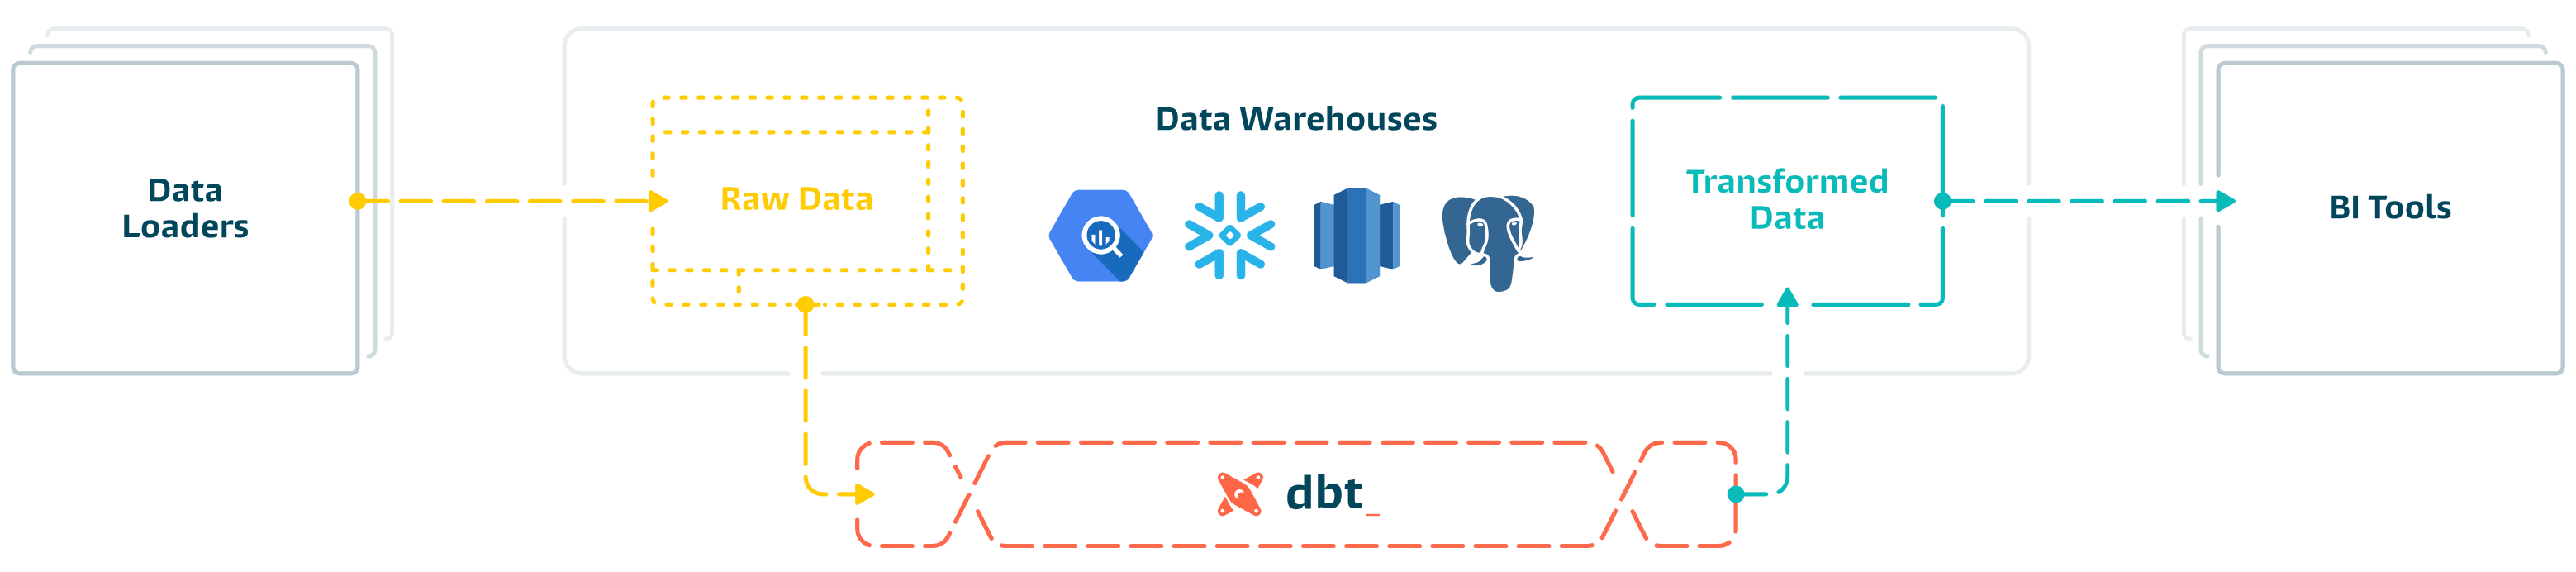
\includegraphics{./images/dbt.png}
\caption{The role of dbt}
\end{figure}

Source: \href{https://www.startdataengineering.com/post/advantages-of-using-dbt-data-build-tool/}{Reference}

\hypertarget{the-dbt-architecture}{%
\chapter{\texorpdfstring{The \texttt{dbt} architecture}{The dbt architecture}}\label{the-dbt-architecture}}

In my first time working with dbt, I was overwhelmed with its architecture. It felt like that individual who is sitting before that large screen in a nuclear power plant and in charge of all the controls. Nevertheless, if people can gain confidence in holding a nuclear power plant on their fingertips, then surely you can crack dbt.

The main components that make up dbt are as follows:

\begin{itemize}
\item
  models
\item
  tests
\item
  documentation
\item
  sources
\end{itemize}

Let's go through each one.

\hypertarget{models}{%
\section{Models}\label{models}}

This is the component of dbt that you will most likely work with. In dbt, a model is simply a SQL statement. As simple as that. dbt will use the SQL statements to perform the transformations in your data warehouse that have been defined in your SQL statement. For example, say I want to create a new column of the table in my Google BigQuery. I will create a SQL statement that does just that. That SQL statement is what is referred to as a model in dbt.

Below is an example of a model that creates a table called \texttt{customers}. The model is saved as \texttt{customers.sql}.

\begin{verbatim}
with customer_orders as (
    select
        customer_id,
        min(order_date) as first_order_date,
        max(order_date) as most_recent_order_date,
        count(order_id) as number_of_orders

    from jaffle_shop.orders

    group by 1
)

select
    customers.customer_id,
    customers.first_name,
    customers.last_name,
    customer_orders.first_order_date,
    customer_orders.most_recent_order_date,
    coalesce(customer_orders.number_of_orders, 0) as number_of_orders

from jaffle_shop.customers

left join customer_orders using (customer_id)
\end{verbatim}

\hypertarget{tests}{%
\section{Tests}\label{tests}}

``Do not put me to test'', is a familiar statement from an impatient person. However, dbt allows us to test our data and see if it meets certain assertions. In other words, does our data meet the requirements that have been set for it?

dbt offers two ways to perform your tests:

\begin{enumerate}
\def\labelenumi{\arabic{enumi}.}
\item
  generic, and,
\item
  custom tests.
\end{enumerate}

Generic tests involve just using a pre-defined test that comes packaged in dbt. For example, for every field key you place in a YAML file in dbt, you can specify which kind of test to perform on that particular field from the following options: \texttt{unique}, \texttt{not\_null}, \texttt{accepted\_values} and \texttt{relationships}.

\begin{itemize}
\tightlist
\item
  \texttt{unique} - the values should be radically distinctive all through
\item
  \texttt{not\_null} - there shouldn't be a missing value in the particular column name in the table
  \emph{\texttt{accepted\_values} - only the values contained in the accepted values key will be considered valid. Anything outside of this will result in an error
  }\texttt{relationships} - the values in this field can be referenced in a different column elsewhere in the table or on a different table altogether.
\end{itemize}

An example of a generic test is below:

\begin{verbatim}
version: 2

models:
  - name: orders
    columns:
      - name: order_id
        tests:
          - unique
          - not_null
      - name: status
        tests:
          - accepted_values:
              values: ['placed', 'shipped', 'completed', 'returned']
      - name: customer_id
        tests:
          - relationships:
              to: ref('customers')
              field: id
\end{verbatim}

For custom tests, these involve one creating a SQL model and referencing it in a YAML file using Jinja template language.

For example, here is a custom test written in a SQL file called \texttt{transaction\_limit\_test.sql}.

\begin{verbatim}
-- tests/transaction_limit_test.sql
select user_id, sum(transaction_amount) as total_spent
from {{ ref('transactions') }}
group by user_id
having total_spent > 10000  -- Assuming the limit is 10,000

\end{verbatim}

The test is referenced in a YAML file and called over a column called \texttt{transactions}.

\begin{verbatim}
models:
  - name: transactions
    tests:
      - transaction_limit_test
\end{verbatim}

\hypertarget{documentation}{%
\section{Documentation}\label{documentation}}

Now, the favourite part of dbt, and possibly the easiest is documentation. Documentation is the description of various components of your data. To write a description of any piece of your data, the \texttt{description} key is used.

For example here is a description of a field called \texttt{event\_id} inside a YAML file.

\begin{verbatim}
version: 2

models:
  - name: events
    description: This table contains clickstream events from the marketing website

    columns:
      - name: event_id
        description: The D-day is the Deed day
        tests:
          - unique
          - not_null
\end{verbatim}

Documentation will be performed where you have placed your tests. There is also a more complex, but scalable manner of writing descriptions. It uses jinja template tags. It works well for large data where the descriptions are many or the descriptions are shared across several tables.

A short example of the jinja templates' documentation is shown below. The description is within a markdown file (\texttt{.md}) other than the one containing my field names. The descriptions will be like so:

\begin{verbatim}


I am not so very robust, but I’ll do the best I can.

Some text here

1) and here
2) and here
3) and also here


\end{verbatim}

So when one returns to their YAML file, they will reference the particular field of interest with the above description like so:

\begin{verbatim}
version: 2

models:
  - name: events
    description: '{{ doc("table_events") }}'

    columns:
      - name: event_id
        description: The D-day is the Deed day
        tests:
            - unique
            - not_null
\end{verbatim}

\hypertarget{sources}{%
\section{Sources}\label{sources}}

\texttt{sources} enable one query the data in your data warehouse. Once you specify the existing table in your data warehouse under the \texttt{sources} key, you can access every data from within this table using SQL. To work with a source table, you first have to wrap it inside a \texttt{\{\{\ source(table-name)\ \}\}} jinja template. Below is an example of how to declare a source.

\begin{verbatim}
version: 2

sources:
  - name: jaffle_shop
    database: raw  
    schema: jaffle_shop  
    tables:
      - name: orders
      - name: customers

  - name: stripe
    tables:
      - name: payments
\end{verbatim}

You can reference the above source inside a SQL model like so:

\begin{verbatim}
select
  ...

from {{ source('jaffle_shop', 'orders') }}

left join {{ source('jaffle_shop', 'customers') }} using (customer_id)

\end{verbatim}

dbt will thereafter know that it will perform some operations using data from the \texttt{orders} and \texttt{customers} data from the \texttt{jaffle\_shop} --the origin of all our data in this example.

\hypertarget{data-storage}{%
\chapter{Data storage}\label{data-storage}}

As as been repeatedly mentioned, to the point of boredom, dbt transforms the data in your data warehouse. Now, before expanding the concept of a data warehouse, the following two are also terms you will hear mentioned quite often in the field of data engineering. They are data lake and data lakehouse.

\hypertarget{data-warehouse}{%
\section{Data warehouse}\label{data-warehouse}}

At the very beginning, when introduced to data engineering concepts with a test paper to boot in four weeks time, I thought that a data warehouse was some storage system akin to that found in Google Drive. I could have been partly right, but I was still far off the mark. A data warehouse is more than just a storage system. It is where data is not only stored but also queried, by means of SQL. It allows data from multiple sources such as internet of things, apps, from emails to social media and keeps a historical record of any changes. Examples of data warehouses are Snowflake, Google Big Query, Amazon Redshift and Azure Synapse Analytics.

The following are the components of a data warehouse.

\begin{enumerate}
\def\labelenumi{\arabic{enumi}.}
\item
  Data sources - this refers to the origins of the data that lands in your data warehouse.
\item
  Extract, Transform and Load (ETL) Processes - these are the processes involved in extracting, transforming and loading the data into your data warehouse.
\item
  Data warehouse database - this is the central repository where the cleansed, integrated and historical data is stored.
\item
  Metadata repository - metadata is essentially data about data. Metadata will typically contain the source, usage, values and other features that comprise your data.
\item
  Access tools - imagine having to figure a way how to write a document in your computer without Microsoft Word. How hard would that be? Access tools are similar to Microsoft Word. They are the tools that enable a user to interact with the data. They include querying, reporting and visualization tools.
\end{enumerate}

As you can see from above, a data warehouse is more than just a storage area for your data. It is like a whole community that will provide the services that you desire, so long as they are integrated into the data warehouse.

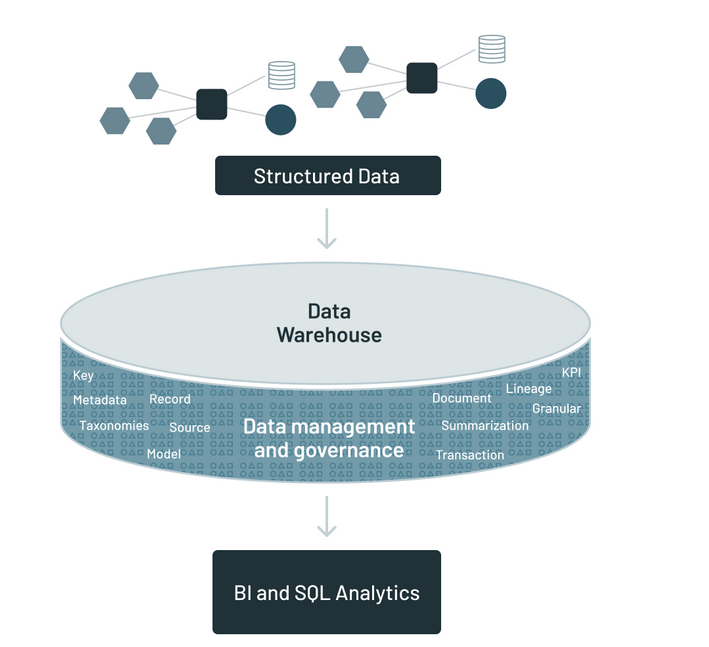
\includegraphics{./images/data_warehouse.png}
Source: \href{https://www.databricks.com/blog/2021/05/19/evolution-to-the-data-lakehouse.html}{Reference}

\hypertarget{data-lake}{%
\section{Data lake}\label{data-lake}}

A data lake is a centralized repository that ingests and stores large volumes of data in its original form. Due to its open, scalable architecture, a data lake can store structured (database tables, excel sheets), semi-structured (xml, json and web pages) and unstructured data (images, audio, tweets) all in one place. Data in the data lake is stored in its original format.

So if data lakes and data warehouses store data, then what is the difference? For one, a data lake can store data of any type, so long as it falls within the three classes of structured, semi-structured and unstructured data. On the other hand, data warehouses deal with more standardized data. That is, data in a data warehouse has undergone some refinement of some kind to be in a structure that fits the organizations's goals.

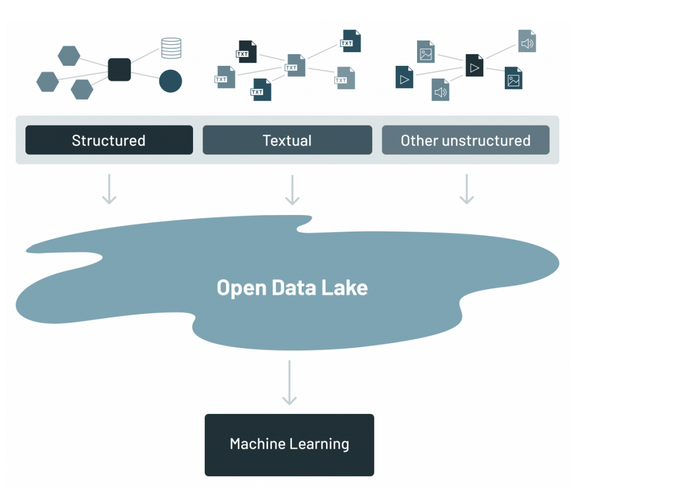
\includegraphics{./images/data_lake.png}
Source: \href{https://www.databricks.com/blog/2021/05/19/evolution-to-the-data-lakehouse.html}{Reference}

\hypertarget{data-lakehouse}{%
\section{Data lakehouse}\label{data-lakehouse}}

A data lakehouse is simply a hybrid of a data warehouse and data lake. It is like a product that combines the best of both worlds. A data lakehouse provides both scalability of large sums of data from the data lake and additionally, the application of a structural schema to data inherent in data warehouses.

Even with the above definition, it is still hard to decipher the advantage that a data lakehouse offers above that of a data warehouse. Apart from allowing the querying of unstructured data, storage costs are lower in a data lakehouse compared to a data warehouse.

\begin{figure}
\centering
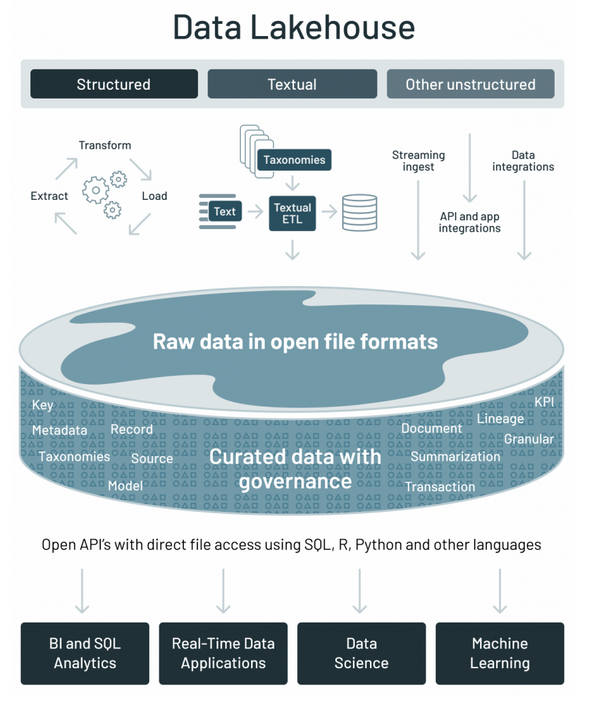
\includegraphics{./images/data_lakehouse.png}
\caption{Data lakehouse}
\end{figure}

Source: \href{https://www.databricks.com/blog/2021/05/19/evolution-to-the-data-lakehouse.html}{Reference}

\hypertarget{a-brief-history}{%
\section{A brief history}\label{a-brief-history}}

At the very beginning, companies used to rely on relational databases and these were sufficient. However, they became too numerous as the needs and services of companies grew. Therefore, experts decided to look for a way of how they could merge all these single databases into one repository which would hold everything while allowing for permission controls to who gets access to what. Believe it or not, the concept of the data warehouse began in the 1960s but it is in the 1980s and 1990s that interest in this topic really began to get traction. That's until the need for storing unstructured data from emails, images and audio began to grow. Data warehouses were not so efficient in storing this thanks to their strict schema enforcement (read, they store data in a structured format).

The beginning of 2000s saw the rise in the need to properly manage unstructured data with the growth of online platforms such as Google and Yahoo. Companies needed a way to store and retrieve unstructured data quickly and efficiently, which wasn't possible with data warehouses. Data lakes excelled in storing all sorts of raw data, from structured to unstructured and everything in between. If you read on the history of data lakes, you willquite often come across the word `Hadoop'. Hadoop is the pioneer of the data lakes we use today.

However, despite being a good storage for any sort of data, the pesky question of maintaining some quality and order resurfaced again! How could we maintain some structure while allowing the data to be in any structure?!

From 2010s and onwards, after a decade of success with data lakes, companies wanted a better storage system from which to run their machine learning models but had the best capabilities of both a data warehouse and a data lake. Before lakehouses, companies would first ingest data into a data lake, then load into a data warehouse from where analytics would be done. But how could we just merge it into one place where storage and analytics could happen? This is how the data lakehouse concept came to be. Data lakehouses provide the following benefits:

\begin{enumerate}
\def\labelenumi{\arabic{enumi}.}
\item
  ACID (Atomicity, Consistency, Isolation and Durability) transactions - ACID transactions promote integrity during data transfer.
\item
  Delta lake - initially developed by the Databricks team, this is a layer on top of your data in the data lake that provides a schema, keeps a record of changes in your data (versioning) and stores metadata.
\item
  Machine learning support - because a data lakehouse can store more data types than the data warehouse, it is a better place to perform machine learning modeling.
\end{enumerate}

For more information on the evolution of data storage systems, this is a \href{https://www.databricks.com/blog/2021/05/19/evolution-to-the-data-lakehouse.html}{definitive guide}.

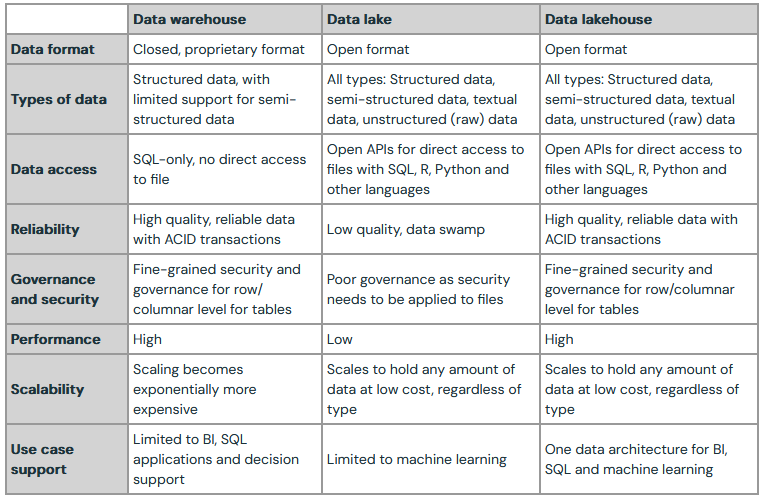
\includegraphics{./images/data_storages.png}
Source: \href{https://www.databricks.com/blog/2021/05/19/evolution-to-the-data-lakehouse.html}{Reference}

\hypertarget{our-data-in-bigquery}{%
\chapter{Our data in BigQuery}\label{our-data-in-bigquery}}

In an earlier chapter, we saw that in data engineering data mainly goes through three processes: extract, load and transform (ELT). The Extract, Transform, Load (ELT) is more of a traditional approach and we will not use it in this case. We will be using Google Bigquery as our data warehouse when working with dbt.

As a reminder, let's go through the definitions of ELT.

Extract - the process of identifying and reading data from one or more source systems. We won't have to do this since the New York City (NYC) bikes data that will be using has already been \emph{extracted} from its source by BigQuery creators.

Load - the process of adding the extracted data to the data warehouse, --in this case Google BigQuery. Again, Google has done this for us. Therefore we won't have to do it.

Transform - the process of converting data from its raw format to the format that it will be used for analysis. This falls definitely within our forte. And we shall use dbt for this. Examples of data transformations that can be done with SQL modeling in dbt are:

\begin{itemize}
\tightlist
\item
  Replacing codes with values
\item
  Aggregating numerical sums
\item
  Applying mathematical functions (SQL can do some maths too, but can be very verbose here)
\item
  Converting data types
\item
  Modifying text strings
\item
  Combining data from different tables and databases.
\end{itemize}

\hypertarget{accessing-big-query}{%
\section{Accessing Big Query}\label{accessing-big-query}}

BigQuery is a data warehouse provided by Google.

To access it, open an incognito window and go to this \href{https://cloud.google.com/}{link}. Sign in using your gmail account.

Click on \textbf{Console} button at the top right. That step of bravery will take you to an interface that looks like this:

\begin{figure}
\centering
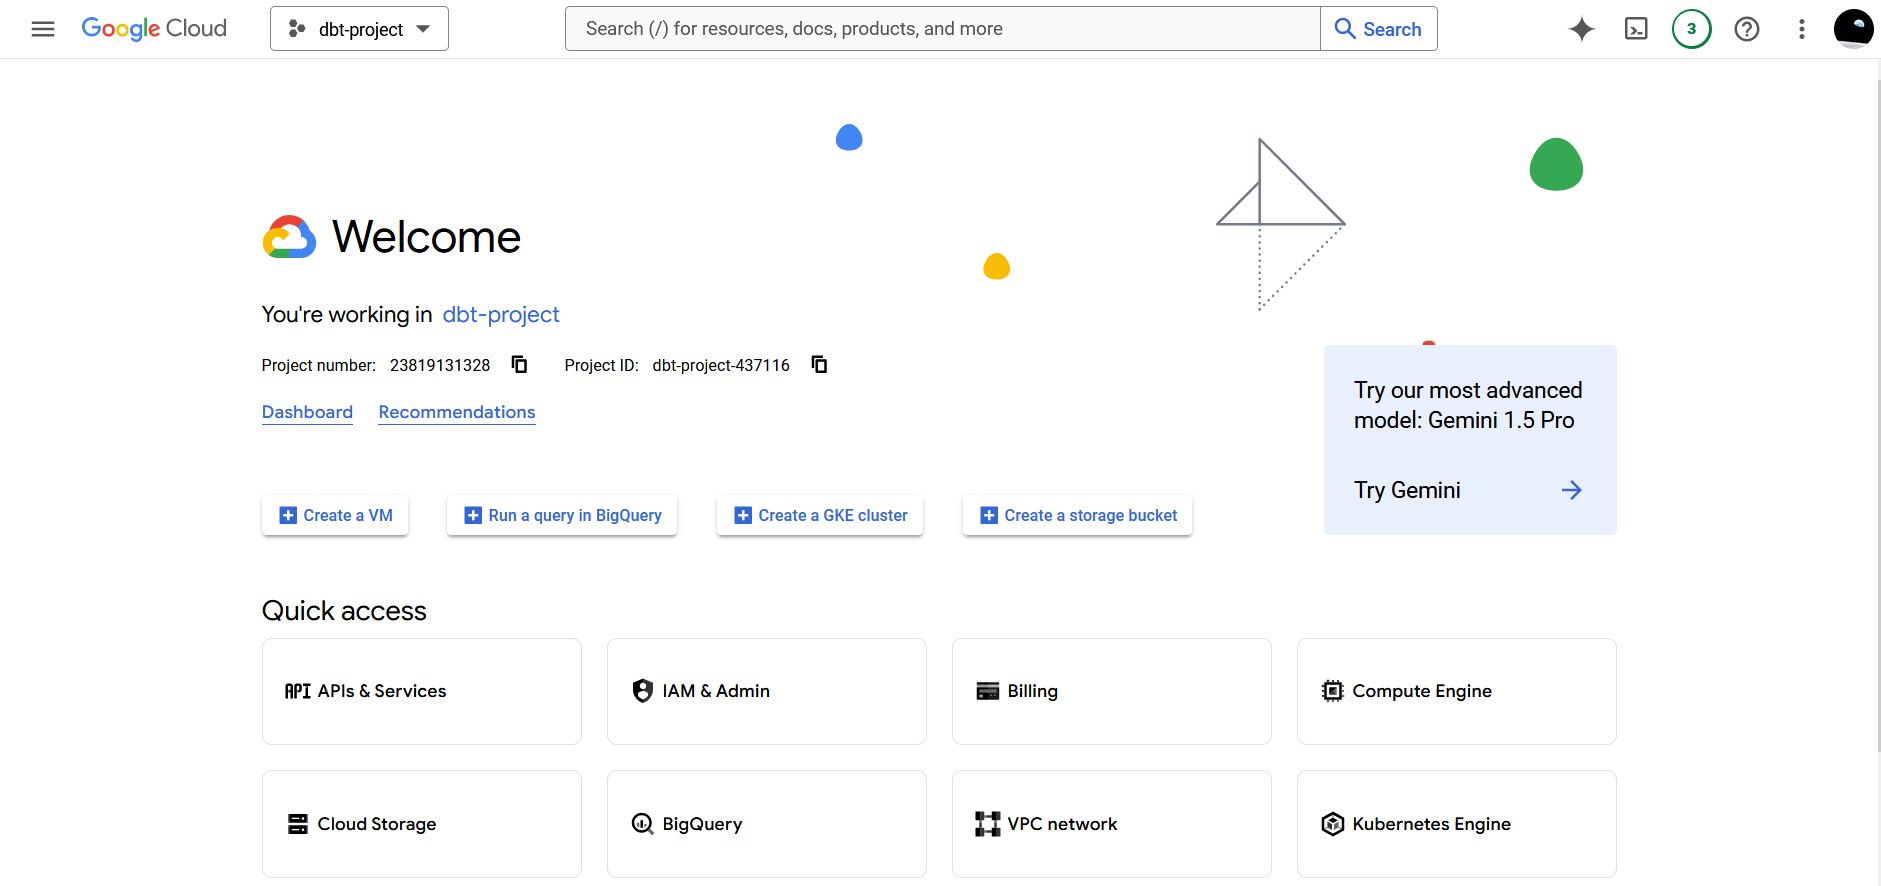
\includegraphics{./images/gcp_interface.png}
\caption{GCP Interface}
\end{figure}

Click on the dropdown at the top. Select \textbf{NEW PROJECT}. We want to create a new project that will contain some tables that we will work with in dbt.

Name your project as \texttt{dbt-project1} or any other name you prefer. Then select \textbf{CREATE}.

Once the project has been created, you will be returned to the original page as at first. However, when you select the project dropdown again, you should see your newly created project as one of the options.

\begin{figure}
\centering
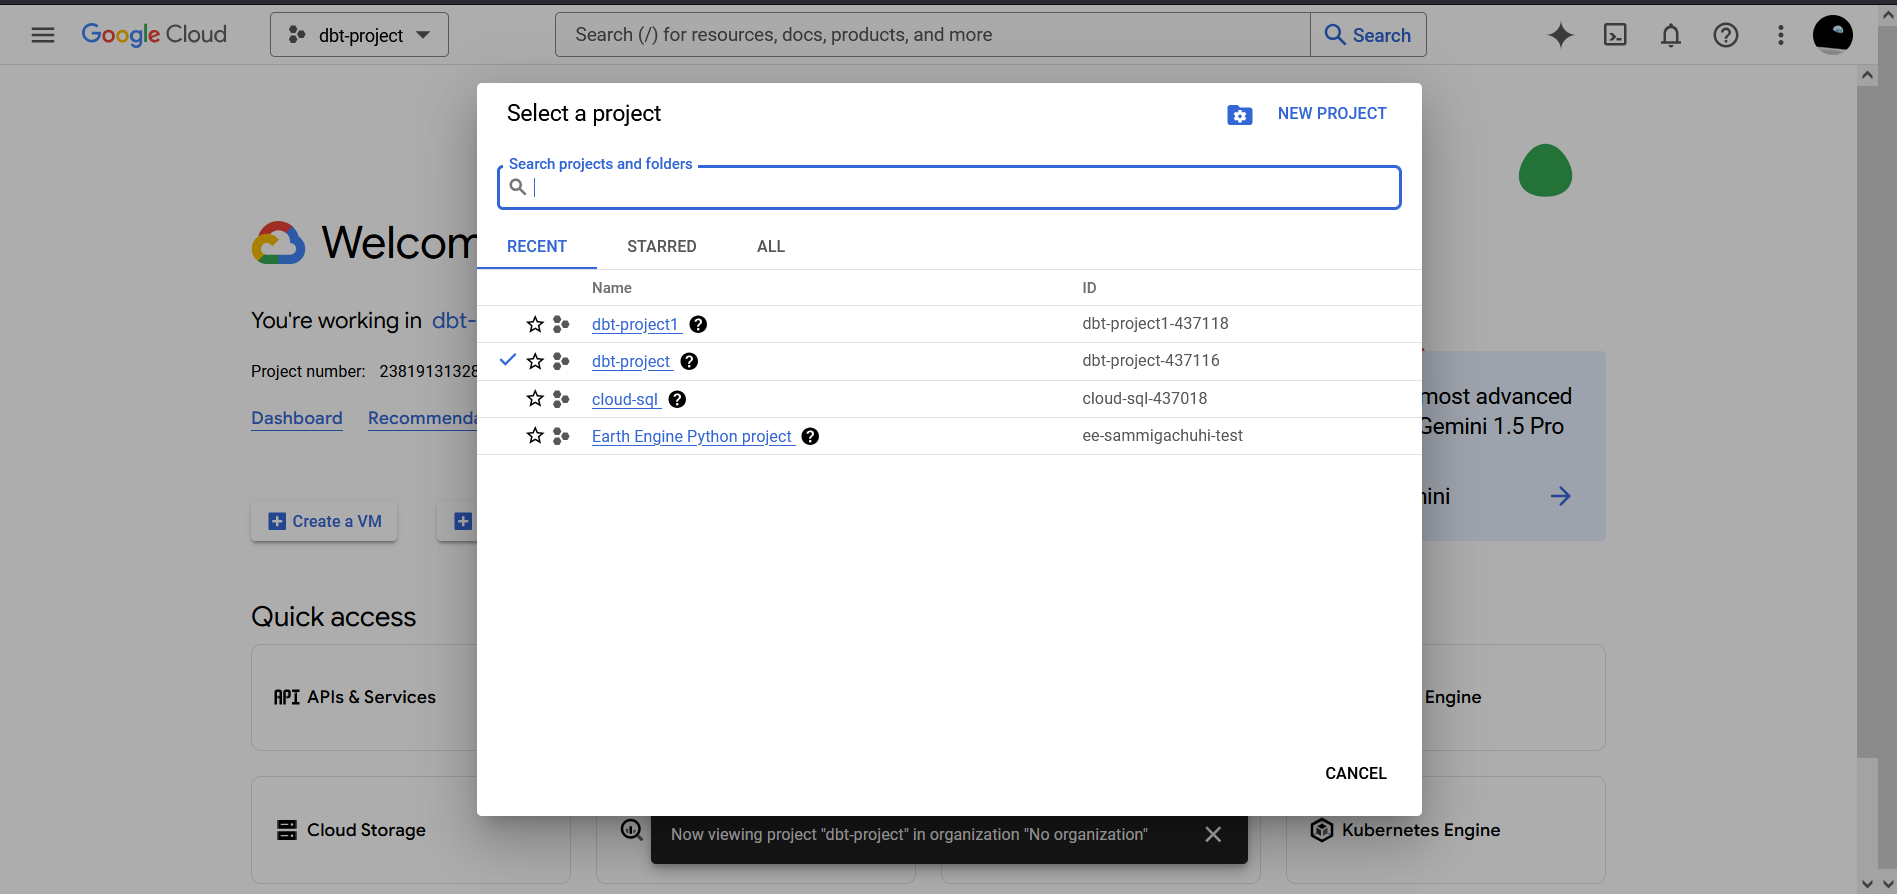
\includegraphics{./images/gcp_project.png}
\caption{GCP Project}
\end{figure}

Click on your project, the interface will refresh and the dropdown should now reflect \texttt{dbt-project1}.

Click on the \textbf{Dashboard} link on the homepage.

The below interface should appear. It can seem overwhelming at first. Lots of things in one place.

\begin{figure}
\centering
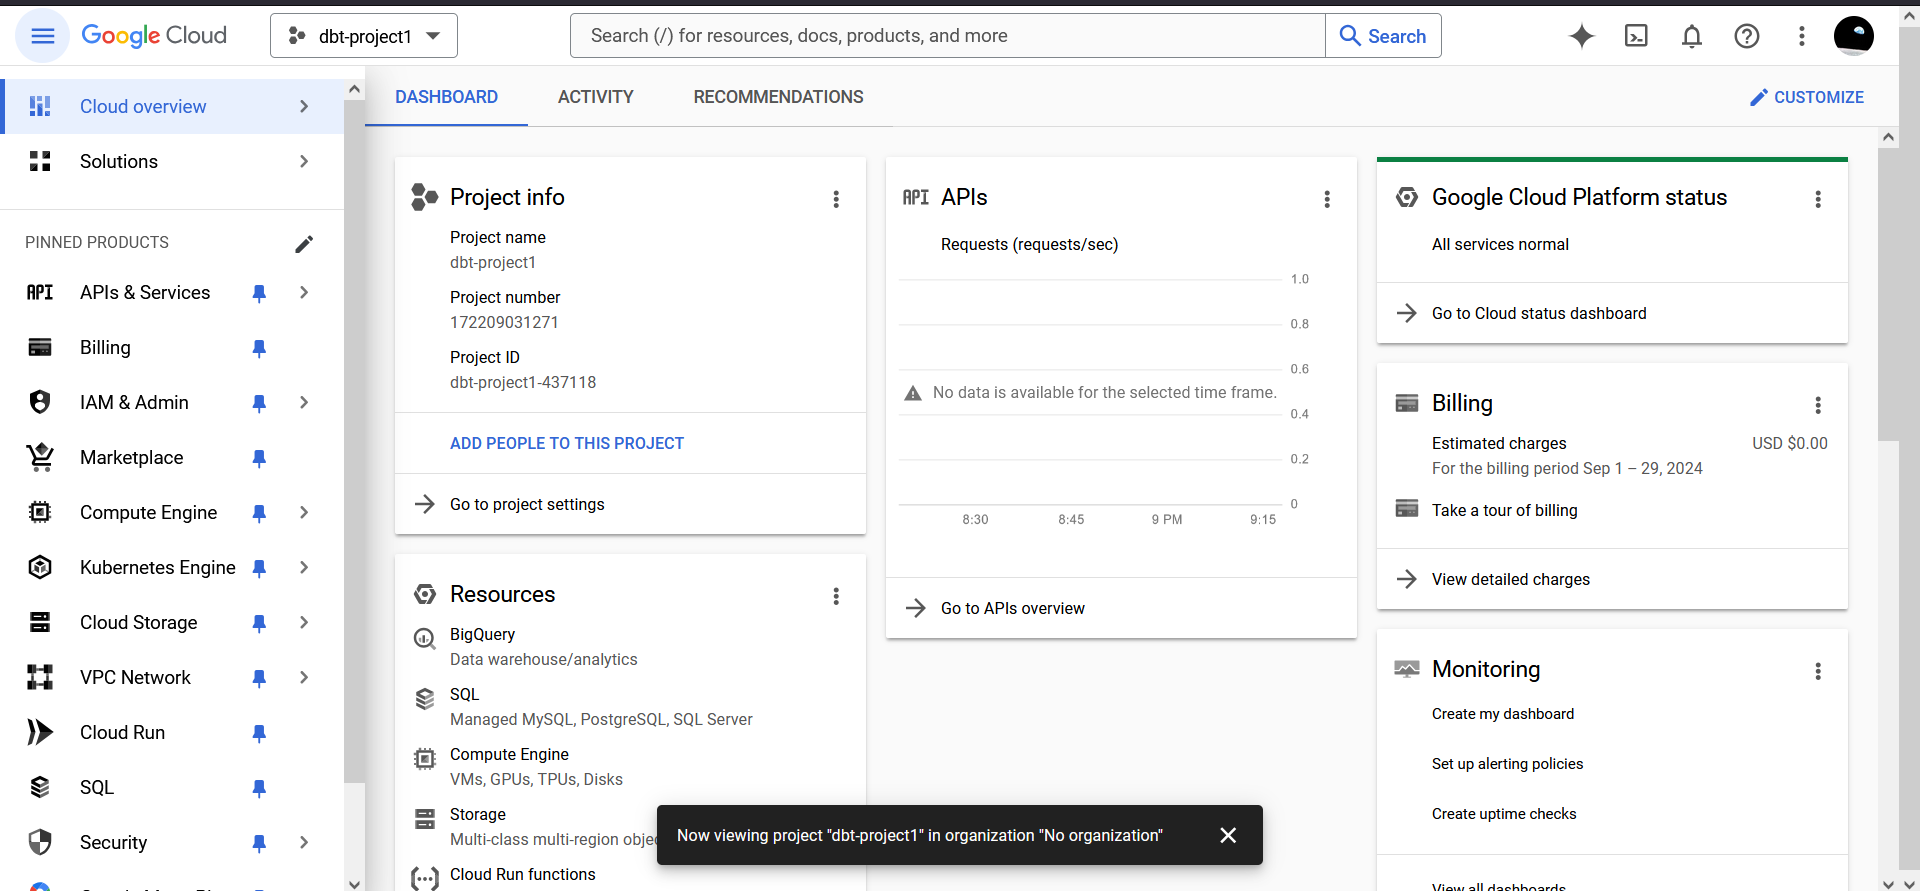
\includegraphics{./images/dashboard.png}
\caption{Dashboard}
\end{figure}

In one of the ``boxes'' within the \textbf{Dashboard} tab, you will find one called \textbf{Resources} with the \textbf{BigQuery} button underneath. Click on this button. It will take you to a page asking you to \emph{Enable the BigQuery Application Programming Interface (API)}. Do comply!

Behold, below is the BigQuery interface.

\begin{figure}
\centering
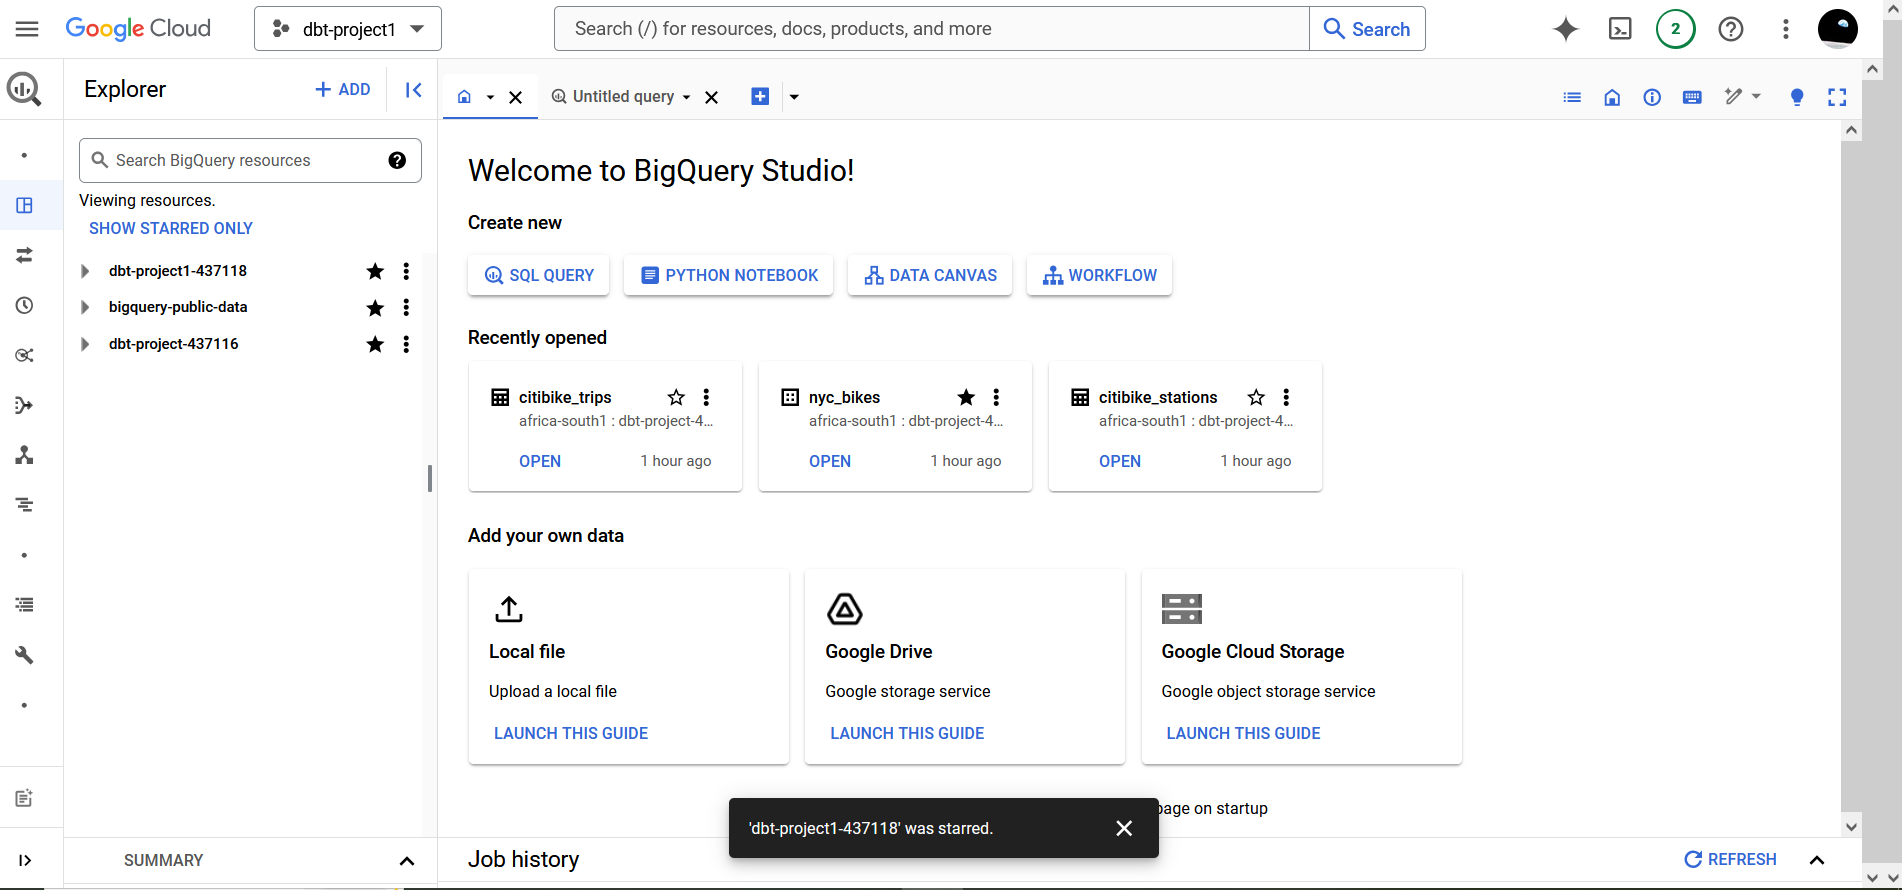
\includegraphics{./images/bigquery_interface.png}
\caption{BigQuery interface}
\end{figure}

You will see one of the resources as \texttt{dbt\_project1\textless{}some-random-number\textgreater{}} in case you had other resources. Star this project for quick access in future.

\hypertarget{copying-the-new-york-city-bikes-data}{%
\section{Copying the New York City Bikes data}\label{copying-the-new-york-city-bikes-data}}

One of the datasets we will be working with is the ``New York City Bikes dataset''. To access it, click on the \textbf{ADD} button. A sidebar will open up. Go to \textbf{Public Datasets}.

In the \textbf{Search Marketplace} searchbar, type `bikes'.

\begin{figure}
\centering
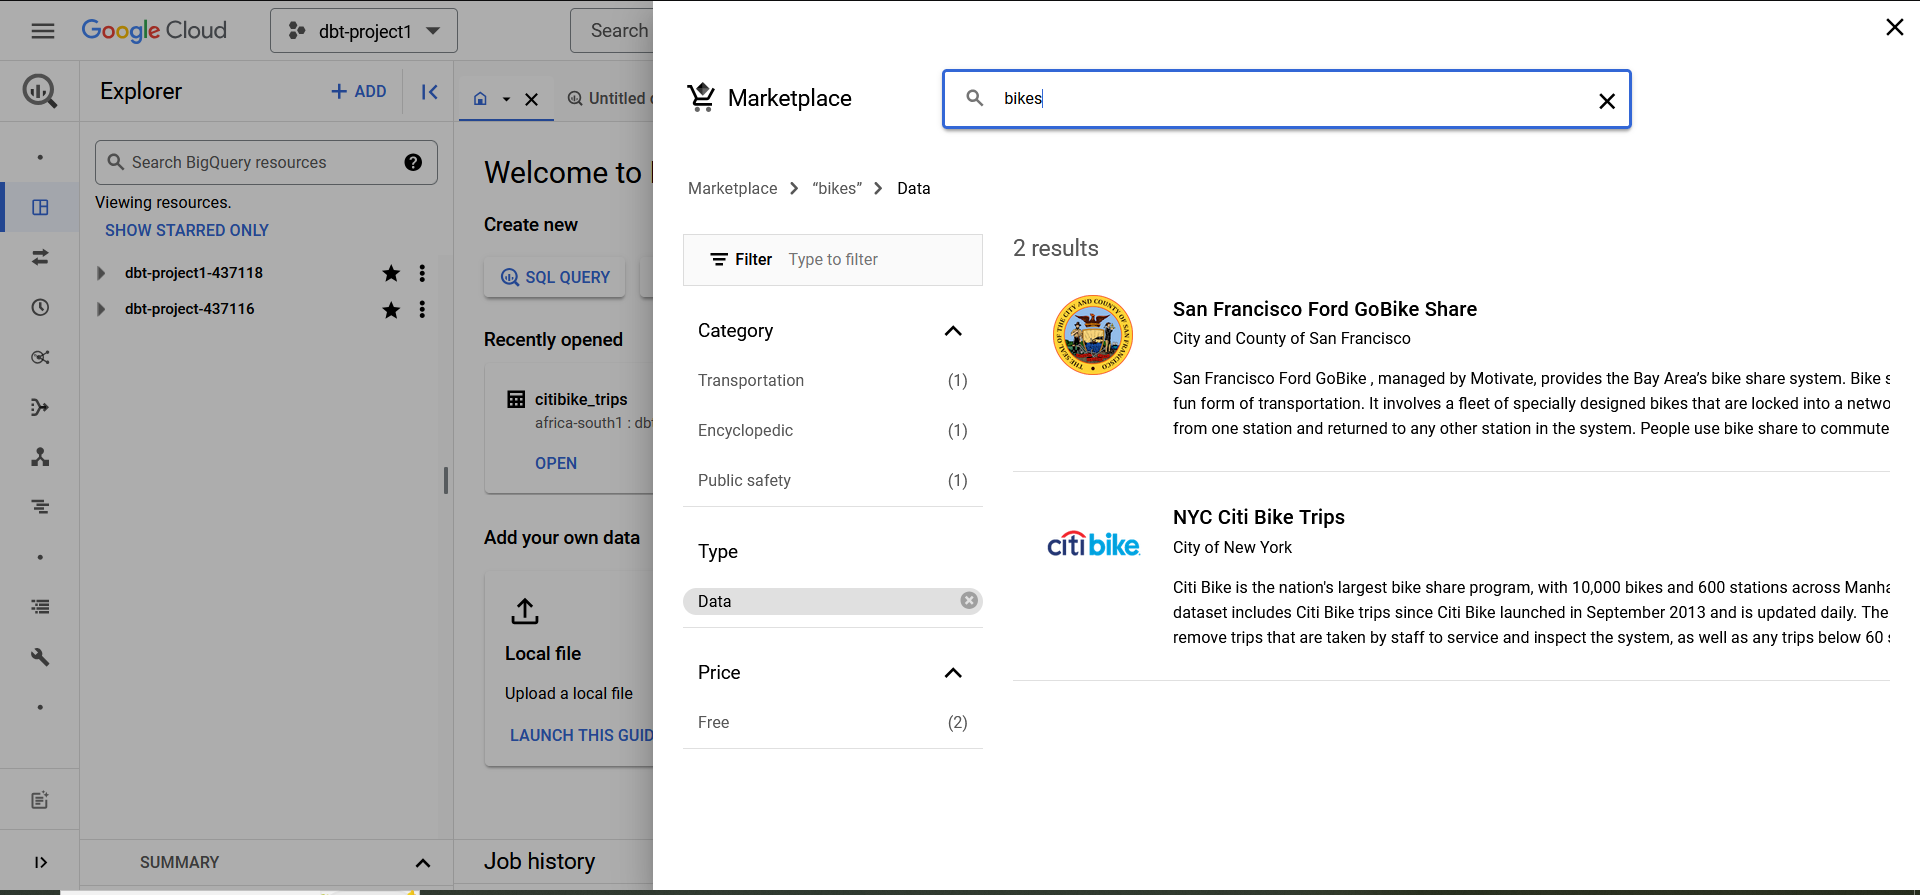
\includegraphics{./images/marketplace.png}
\caption{Marketplace}
\end{figure}

Click on the NYC Citi Bike Trips tab. A new sidebar will popup with a button of \textbf{View Dataset}. Click this button and the Google Cloud Platform (GCP) Dashboard will reappear but this time round the \texttt{bigquery-public-data} resource will appear.

Click on this particular resource's dropdown on the left and scroll down to the \texttt{new\_york\_citibike} dataset. We want to copy this dataset from that of \texttt{bigquery-public-data} to that of \texttt{dbt\_project1-437718}. The random numbers will be different in your case.

Scroll up again to your \texttt{dbt\_project1} resource. On the kebab menu on the right of this resource, select \emph{Create Dataset}.

\begin{figure}
\centering
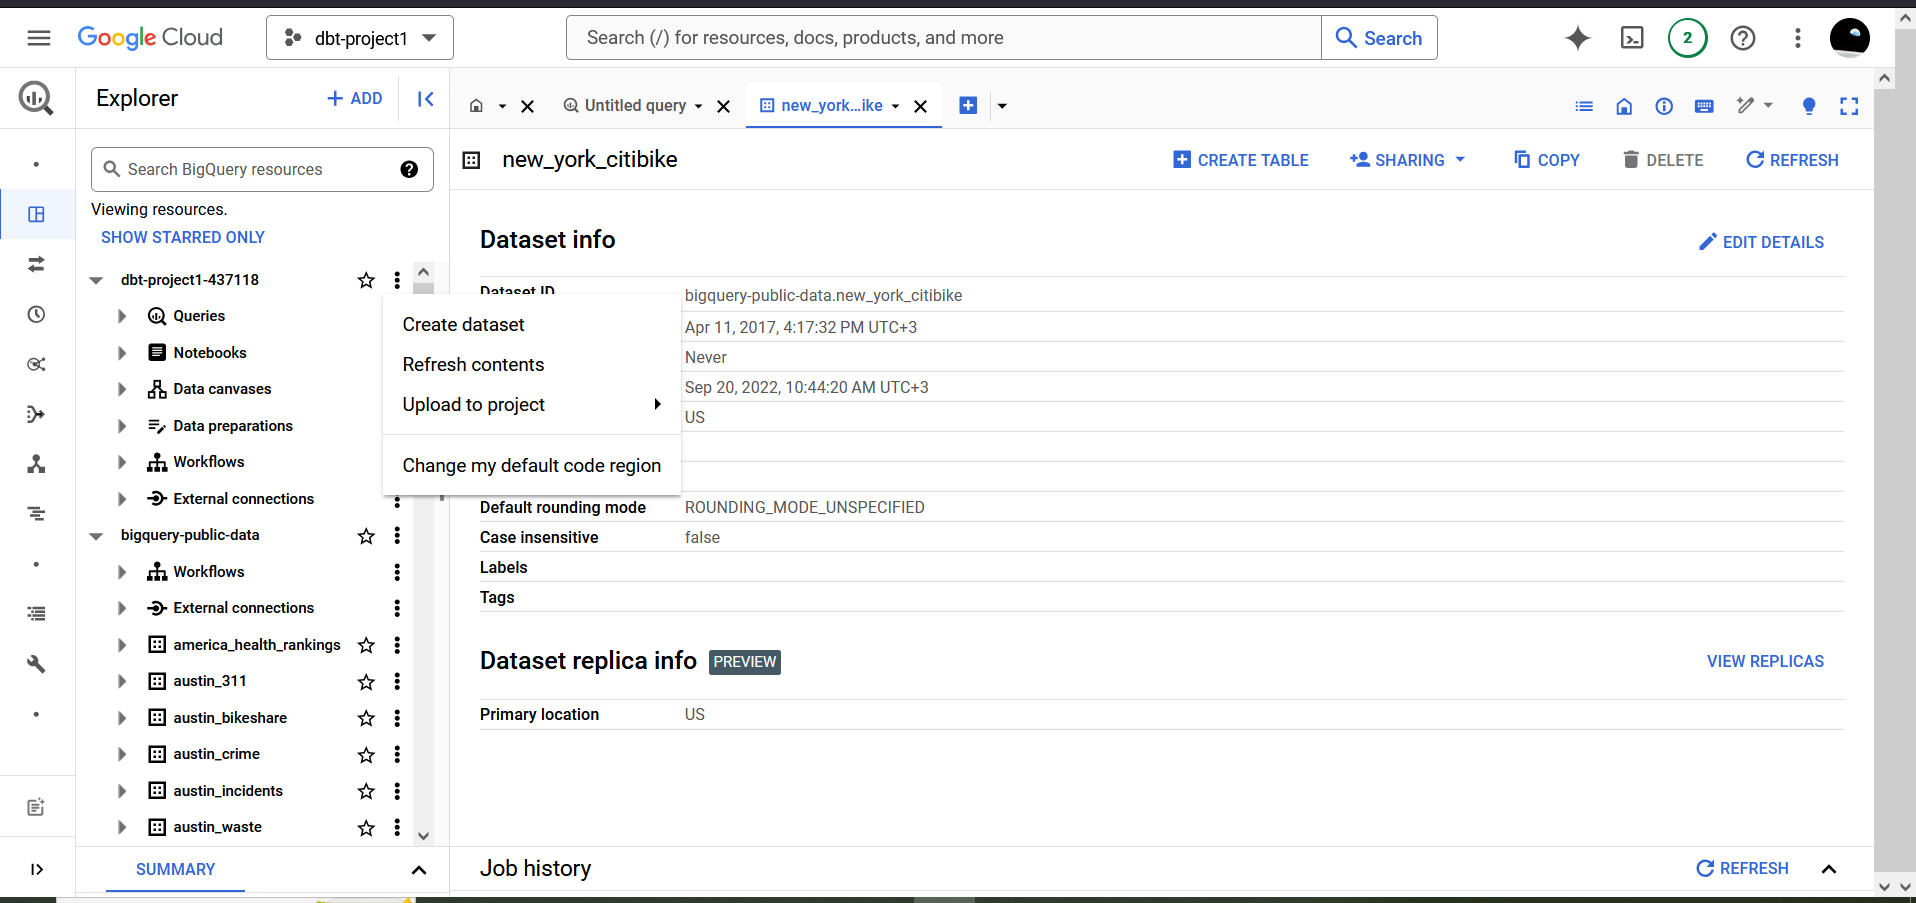
\includegraphics{./images/create_dataset.png}
\caption{Create dataset}
\end{figure}

A new sidebar will open. Insert the following for each parameter:

\begin{itemize}
\item
  Dataset ID - \texttt{nyc\_bikes}
\item
  Location type - \texttt{Region}
\item
  Region - \texttt{africa-south1\ (Johannesburg)} or your preferred region
\end{itemize}

Thereafter, click on \textbf{CREATE DATASET}.

The \texttt{nyc\_bikes} dataset should now appear under the \texttt{dbt-project1} resource. We want to copy the contents of the \texttt{new\_york\_citibike} dataset into our \texttt{nyc\_bikes} dataset. So how do we proceed?

Scroll down to the \texttt{new\_york\_citibike} dataset under the \texttt{bigquery-public-data} resource and click on it. On the menu for this dataset, you will see the \textbf{Copy} button. Click on this button.

\begin{figure}
\centering
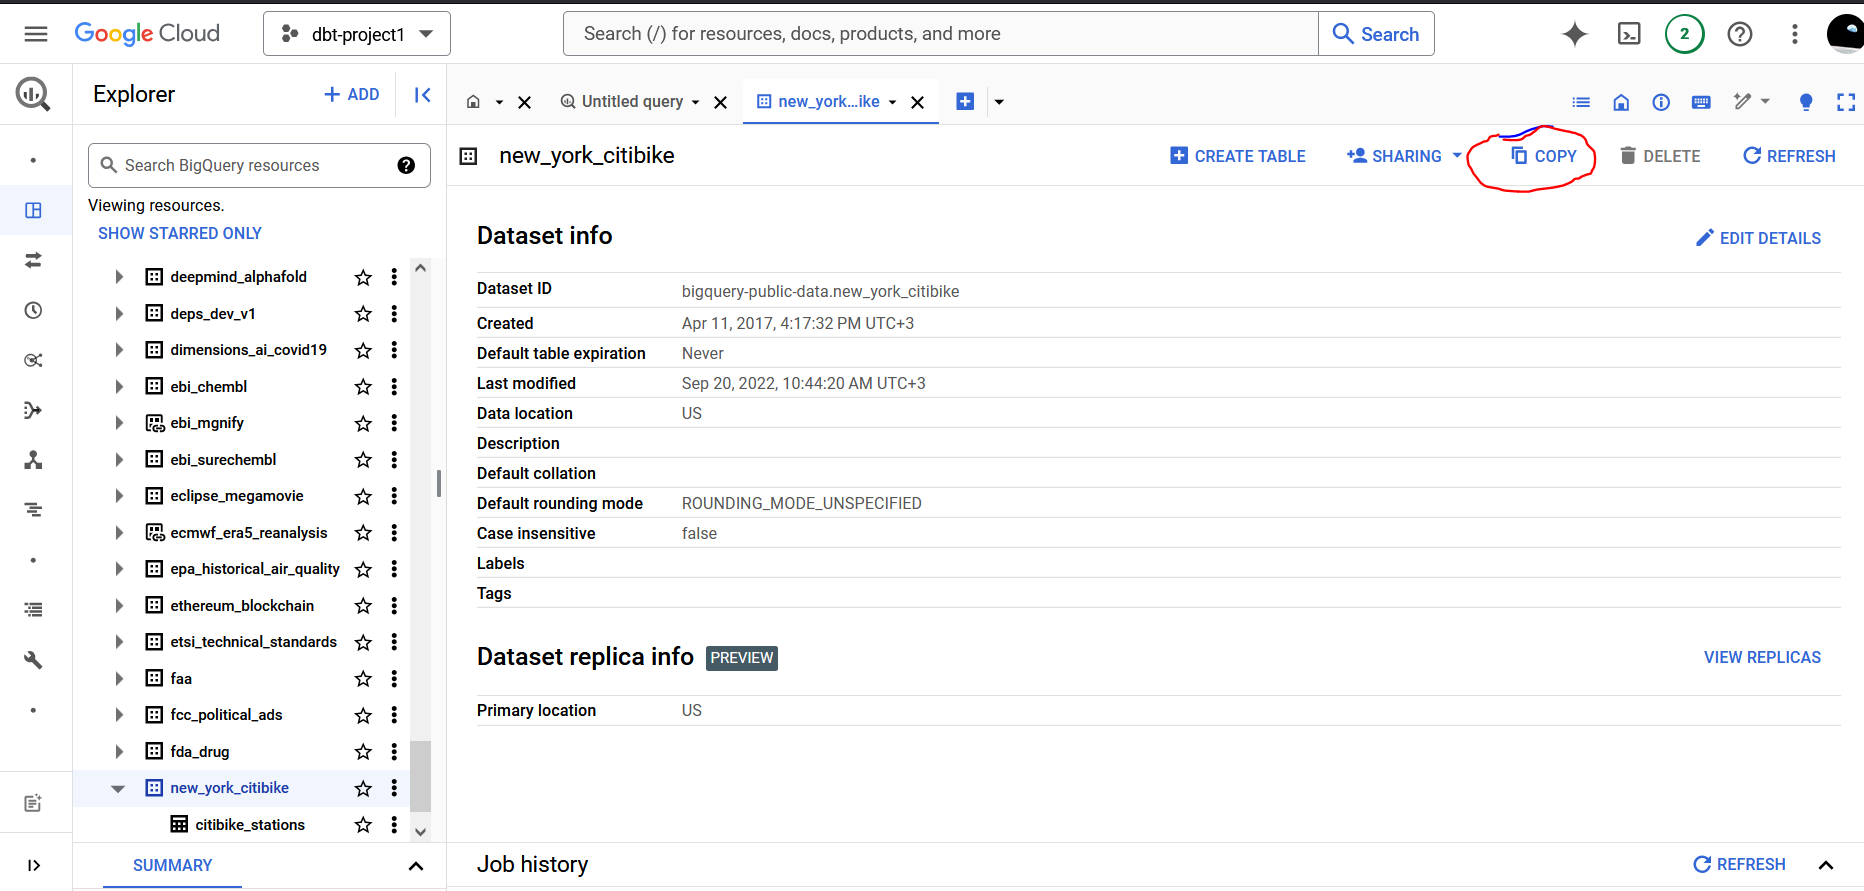
\includegraphics{./images/copy.png}
\caption{Copy dataset}
\end{figure}

\begin{figure}
\centering
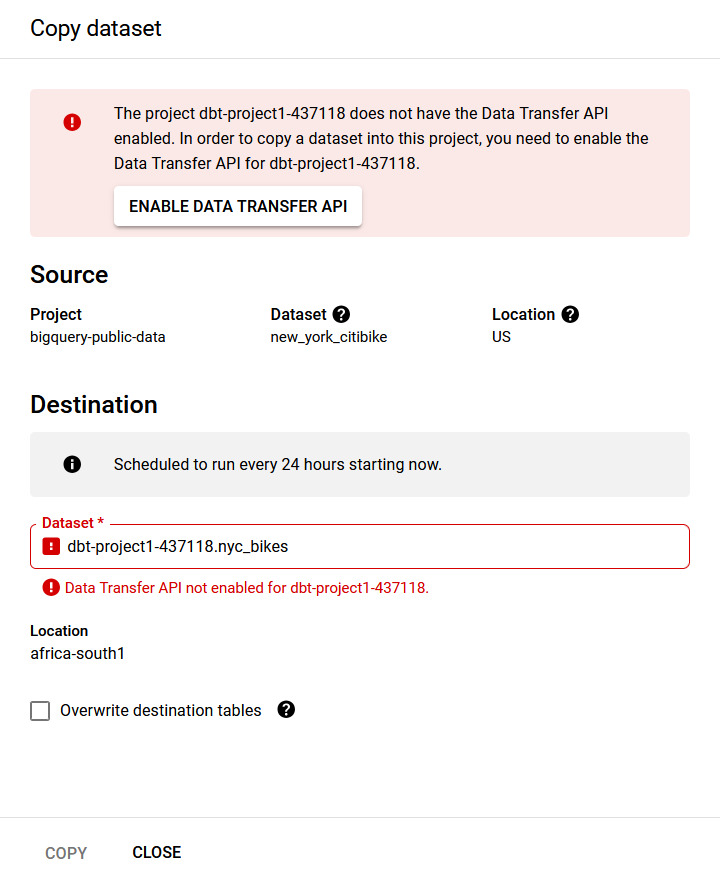
\includegraphics{./images/copy_sidebar.png}
\caption{Copy sidebar}
\end{figure}

In the \textbf{Destination} searchbar, type \texttt{nyc\_bikes} in reference to where we want to copy the contents into. You may need to enable the data transfer API to perform the copy operation. Do so if BigQuery necessitates that \emph{it} must be enabled.

Once you copy the dataset, a small bar will appear on the screen saying \textbf{View Details}. Click on it to stop the run operation since BigQuery will be rerunning the copy operation after every 24 hours. Disable the transfer process and delete it.

Going back to your \texttt{dbt\_project1} resource, your \texttt{nyc\_bikes} dataset should now be having two tables under it. That is:

\begin{itemize}
\tightlist
\item
  citibike\_stations
\item
  citibike\_trips
\end{itemize}

Click on any of the tables and preview the data therein using the \textbf{PREVIEW} button of each tables' interface.

\begin{figure}
\centering
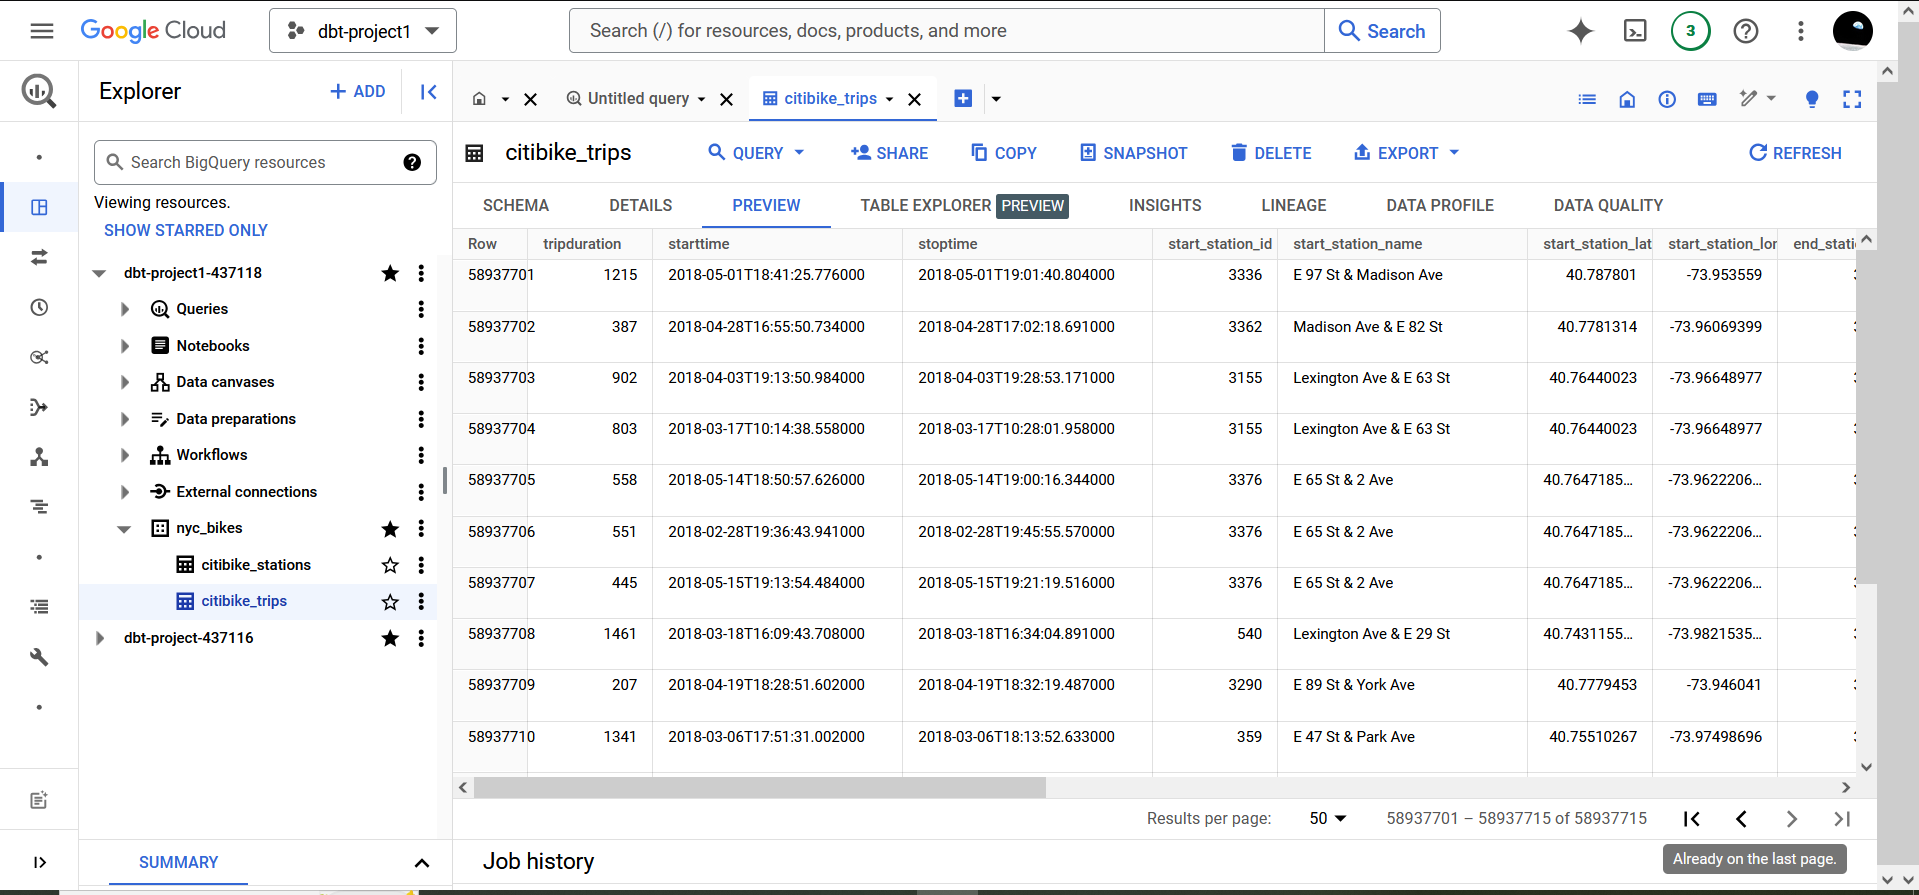
\includegraphics{./images/table_interface.png}
\caption{Table}
\end{figure}

Congratulations on loading your first table in BigQuery!

\hypertarget{installing-dbt}{%
\chapter{Installing dbt}\label{installing-dbt}}

Now that we've seen how to access a dataset inside our data warehouse, now let's proceed to installing dbt. This section assumes you already have Visual Studio (VS) Code installed. All code in this book has been operated within a Linux environment. For Window's users, a Linux environment can be enabled by installing the \href{https://www.freecodecamp.org/news/how-to-install-wsl2-windows-subsystem-for-linux-2-on-windows-10/}{Windows Subsystem for Linux (WSL2)} virtualization platform.

\hypertarget{setting-the-environment}{%
\section{Setting the environment}\label{setting-the-environment}}

Open your VS Code.

Create a new folder called \texttt{dbt\_book}. Move into this directory in your VS Code by typing \texttt{cd\ dbt\_book/} in your terminal.

The first thing we shall do is create a virtual environment from which we shall conduct all our dbt operations. A virtual environment is useful in preventing conflicts between packages across your various programming projects.

\begin{verbatim}
python3 -m venv venv
\end{verbatim}

The first \texttt{venv} tells python that you're creating a virtual environment while the second refers to the name of the virtual environment. In this case, our virtual environment shall still share the name \texttt{venv}.

Now let's activate our virtual environment.

\begin{verbatim}
source venv/bin/activate
\end{verbatim}

You will see your namespace appended with \texttt{venv} which means that your virtual environment is now active. For example:

\begin{verbatim}
(venv) sammigachuhi@Gachuhi:~/dbt_book$ 
\end{verbatim}

Now here comes the big part: installing dbt for Big Query. The following code will install everything we need; both dbt and the dependencies needed to connect it to BigQuery.

\begin{verbatim}
python3 -m pip install dbt-core dbt-bigquery
\end{verbatim}

\hypertarget{connecting-to-your-bigquery-data-warehouse}{%
\section{Connecting to your BigQuery data warehouse}\label{connecting-to-your-bigquery-data-warehouse}}

We wish connecting to a data warehouse for dbt were as easy as providing a username and password. Far from it, but it is definitely possible. To connect dbt to a data warehouse, we use a keyfile. A keyfile is a file that contains encryption keys or licenses for a particular task. The keyfile we shall use shall be the doorway to our data warehouse.

As the first step, go to your \href{https://console.cloud.google.com/apis/credentials/wizard}{GCP Credentials Wizard} page.

Ensure that your project is set to the dbt project you created in the previous chapter. For my case, I reverted to an earlier created project called \texttt{dbt\_project} since my other project \texttt{dbt\_project1} started incurring costs.

For \textbf{Credential Type}:

\begin{itemize}
\item
  From the \textbf{Select an API} dropdown, choose \textbf{BigQuery API}
\item
  Select \textbf{Application data} for the type of data you will be accessing
\item
  Click \textbf{Next} to create a new service account.
\end{itemize}

In the service account page:

\begin{itemize}
\item
  Type \texttt{dbt-book} as the Service account name or any other name you prefer.
\item
  From the \textbf{Select a role} dropdown, choose \textbf{BigQuery Job User} and \textbf{BigQuery Data Editor} roles and click \textbf{Continue}
\item
  Leave the \textbf{Grant users access to this service account} fields blank
\item
  Once everything is fine, it is as good as clicking \textbf{Done}!
\end{itemize}

Your credentials interface will look like this:

\begin{figure}
\centering
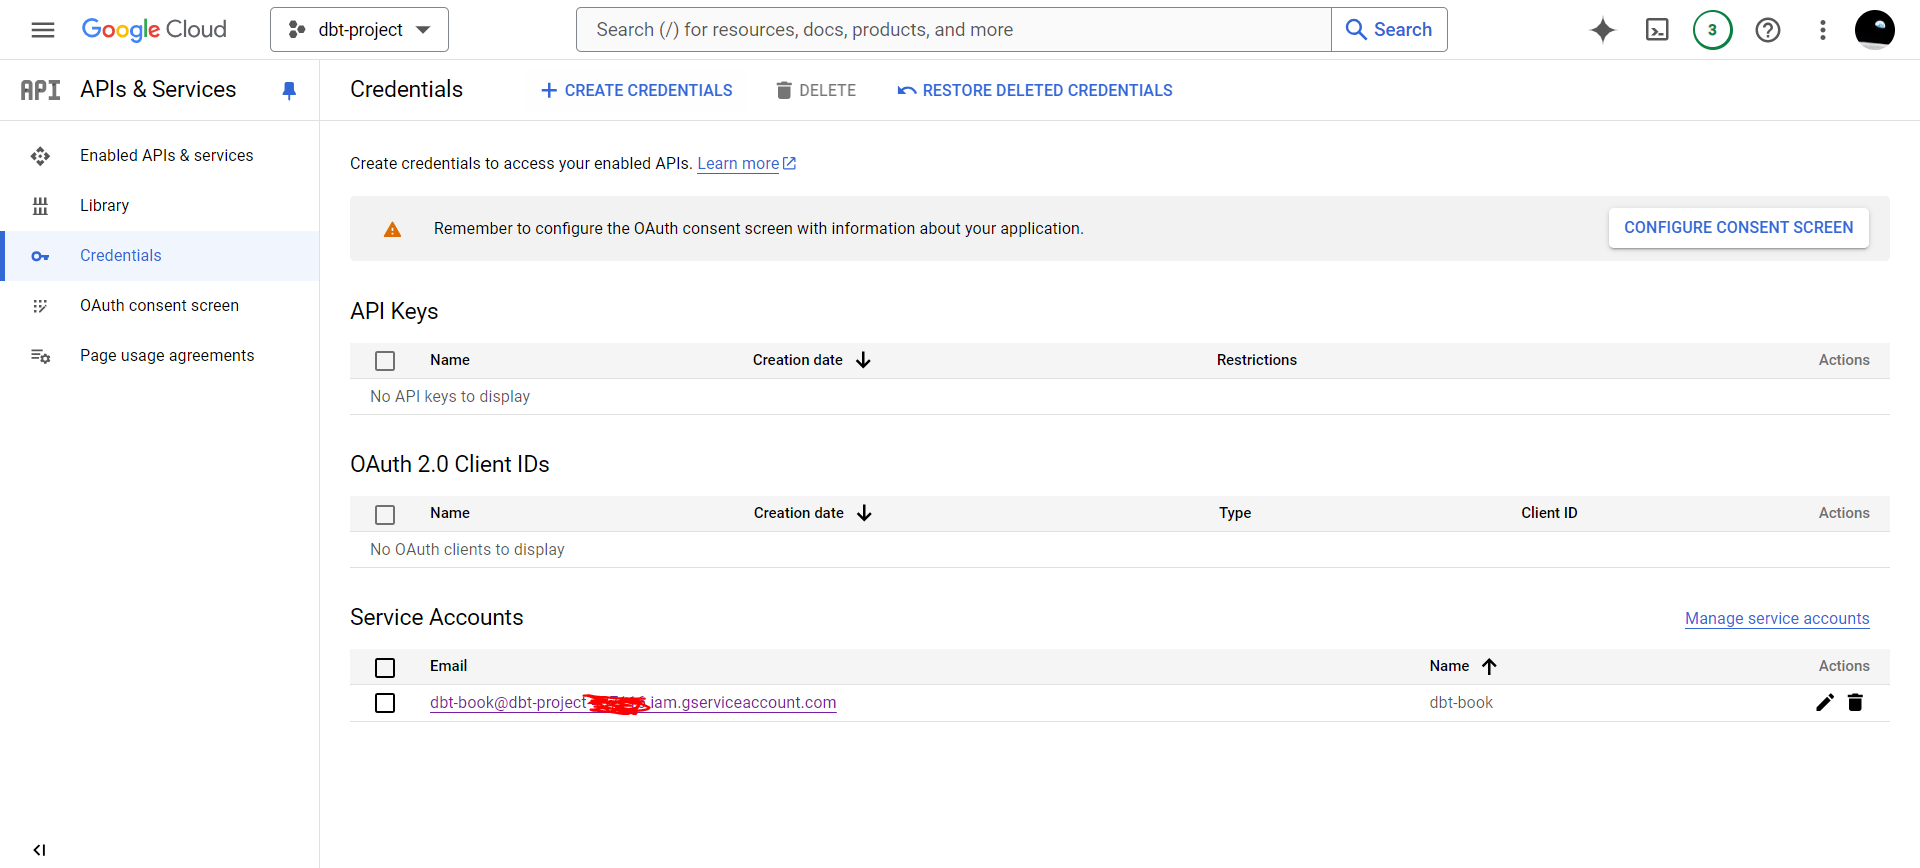
\includegraphics{./images/service-account.png}
\caption{Service account}
\end{figure}

Click on your service account name.

Click on the \textbf{KEYS} tab. We want to create a key that dbt will use to connect to our data warehouse.

Click on \textbf{ADD KEY\textgreater Create new key}.

\begin{figure}
\centering
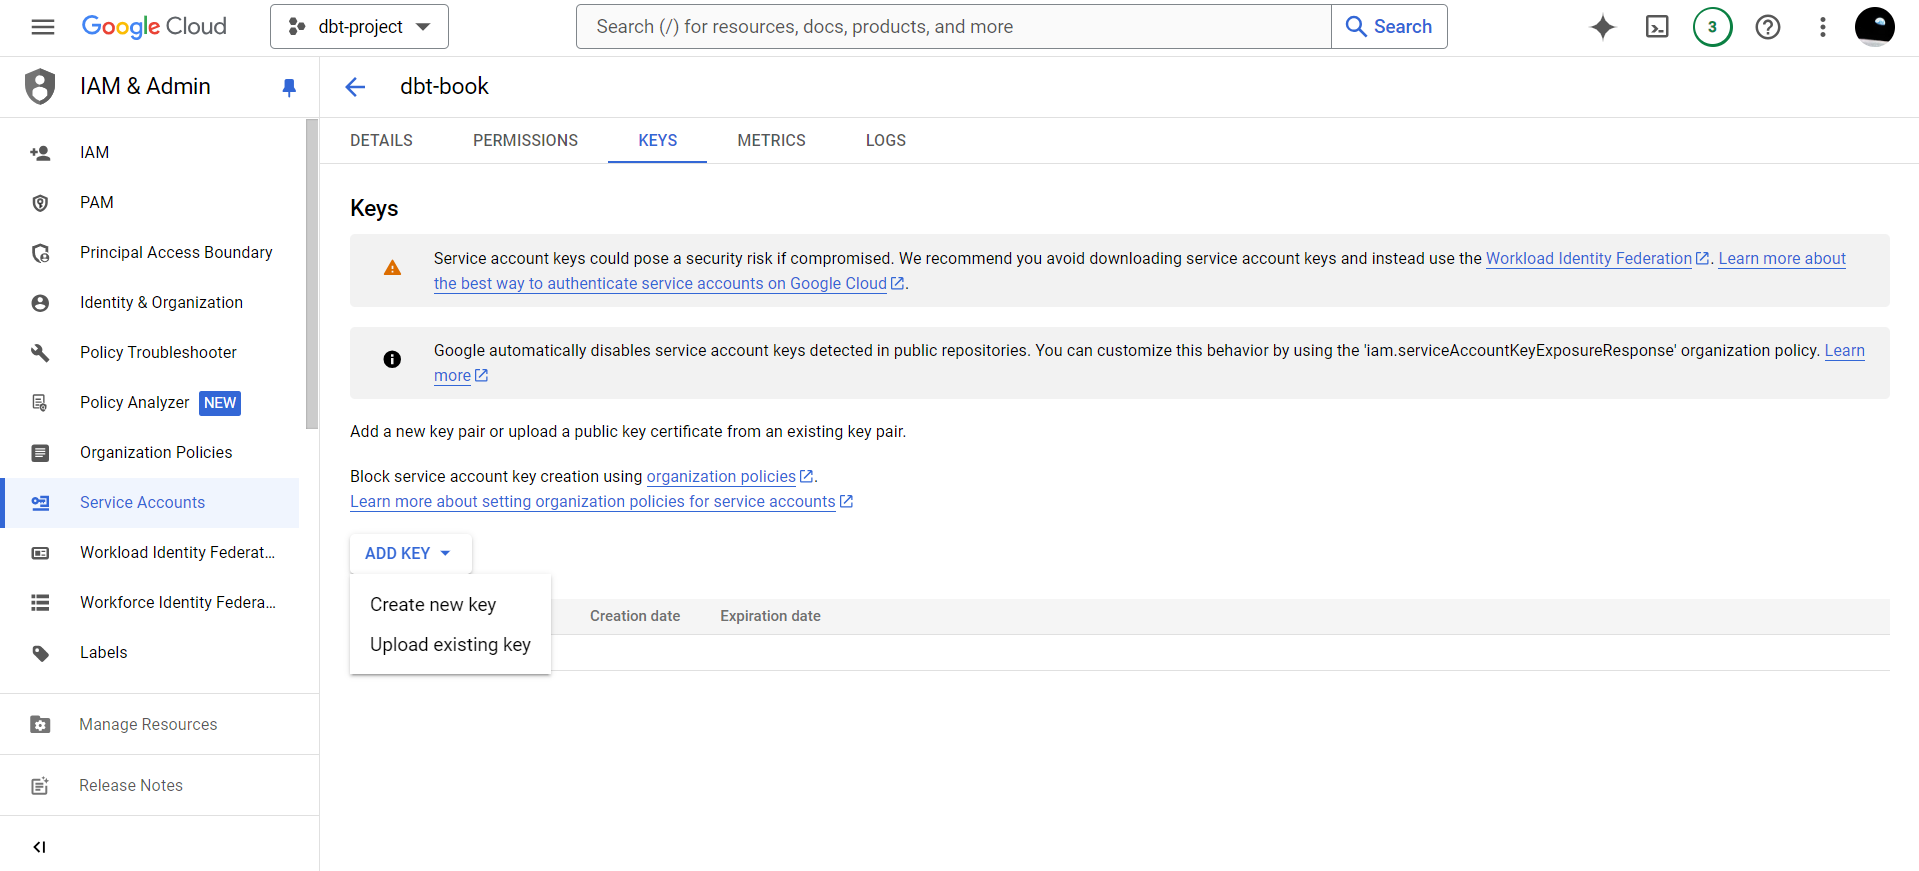
\includegraphics{./images/add-key.png}
\caption{Add key}
\end{figure}

Select \textbf{JSON} on the interface that appears and click \textbf{CREATE}.

This will download a json file containing the encryption keys that dbt will use to connect to your data warehouse.

Store this json file in a safe place.

\hypertarget{initializing-a-dbt-project}{%
\section{Initializing a dbt project}\label{initializing-a-dbt-project}}

To create a dbt project, we run the open sesame key: \texttt{dbt\ init}.

It will create a string of outputs. It's important to key in the right details if you want to create a dbt project.

The first output will ask for the name of your dbt project. Insert \texttt{dbt\_book} or any other name you prefer.

\begin{verbatim}
19:07:31  Running with dbt=1.8.7
Enter a name for your project (letters, digits, underscore): dbt_book
\end{verbatim}

If you had an already pre-existing dbt project with the same name, dbt will ask if it can overwrite that project. Type \texttt{y} if you wish to do so.

dbt will thereafter ask you which database you would like to use. Since we had installed dbt with the package dependancies for BigQuery, you will see the sole option for BigQuery. Type \texttt{1} to select BigQuery.

\begin{verbatim}
Which database would you like to use?
[1] bigquery

(Don't see the one you want? https://docs.getdbt.com/docs/available-adapters)

Enter a number: 1
\end{verbatim}

You will thereafter be asked the authentication method you would like to use. Since we had already created a service account and downloaded the JSON file containing the encryption keys, we shall select option 2.

\begin{verbatim}
Enter a number: 1
[1] oauth
[2] service_account
Desired authentication method option (enter a number): 2
\end{verbatim}

For the keyfile, provide the path to where you had saved the json file. As a note, this path should be somewhere different than where your dbt project is located. Github will set off alarms and send alert emails in case it finds the keyfile within your repository. Keyfiles are never meant to be shared or stored somewhere accessible. They are considered sensitive information.

\begin{verbatim}
keyfile (/path/to/bigquery/keyfile.json): /home/sammigachuhi/dbt_credentials/dbt_book.json
\end{verbatim}

You will also be asked to provide your project ID. This is available under your dbt project's dashboard under the \textbf{Project ID} heading.

\begin{verbatim}
project (GCP project id): dbt-project-437116
\end{verbatim}

For the dataset name, we will use \texttt{nyc\_bikes} which is the dataset we want to conduct our dbt operations on.

\begin{verbatim}
dataset (the name of your dbt dataset): nyc_bikes
\end{verbatim}

For the rest of the options, you can fill them as below:

\begin{verbatim}
threads (1 or more): 1
job_execution_timeout_seconds [300]: 
[1] US
[2] EU
Desired location option (enter a number): 1
19:09:24  Profile dbt_book written to /home/sammigachuhi/.dbt/profiles.yml using target's profile_template.yml and your supplied values. Run 'dbt debug' to validate the connection.
\end{verbatim}

Now, in order to test whether your dbt installation is correct, you will have to change directory (cd) into your \texttt{dbt\_book} subfolder we created as part of the \texttt{dbt\ init} prompts. At first, we had created a directory called \texttt{dbt\_book} in which we also activated the virtual environment. When we ran \texttt{dbt\ init} from this directory, we specified our project name to be \texttt{dbt\_book} as well. It is from here we want to check if our dbt initialization and access to BigQuery was successful.

So move into this subfolder via \texttt{cd\ dbt\_book/}.

\begin{verbatim}
(venv) sammigachuhi@Gachuhi:~/dbt_book$ cd dbt_book/
(venv) sammigachuhi@Gachuhi:~/dbt_book/dbt_book$ dbt debug
\end{verbatim}

Inside the \texttt{dbt\_book} subfolder we created as part of the dbt initialization prompts, run \texttt{dbt\ debug}. If the final output of the run is \texttt{All\ checks\ passed!}, you are good to go!

\begin{verbatim}
19:10:20  Running with dbt=1.8.7
19:10:20  dbt version: 1.8.7
19:10:20  python version: 3.10.12
19:10:20  python path: /home/sammigachuhi/dbt_book/venv/bin/python3
19:10:20  os info: Linux-5.15.153.1-microsoft-standard-WSL2-x86_64-with-glibc2.35
19:10:21  Using profiles dir at /home/sammigachuhi/.dbt
19:10:21  Using profiles.yml file at /home/sammigachuhi/.dbt/profiles.yml
19:10:21  Using dbt_project.yml file at /home/sammigachuhi/dbt_book/dbt_book/dbt_project.yml
19:10:21  adapter type: bigquery
19:10:21  adapter version: 1.8.2
19:10:22  Configuration:
19:10:22    profiles.yml file [OK found and valid]
19:10:22    dbt_project.yml file [OK found and valid]
19:10:22  Required dependencies:
19:10:22   - git [OK found]

19:10:22  Connection:
19:10:22    method: service-account
19:10:22    database: dbt-project-437116
19:10:22    execution_project: dbt-project-437116
19:10:22    schema: nyc_bikes
19:10:22    location: US
19:10:22    priority: interactive
19:10:22    maximum_bytes_billed: None
19:10:22    impersonate_service_account: None
19:10:22    job_retry_deadline_seconds: None
19:10:22    job_retries: 1
19:10:22    job_creation_timeout_seconds: None
19:10:22    job_execution_timeout_seconds: 300
19:10:22    timeout_seconds: 300
19:10:22    client_id: None
19:10:22    token_uri: None
19:10:22    dataproc_region: None
19:10:22    dataproc_cluster_name: None
19:10:22    gcs_bucket: None
19:10:22    dataproc_batch: None
19:10:22  Registered adapter: bigquery=1.8.2
19:10:26    Connection test: [OK connection ok]

19:10:26  All checks passed!

\end{verbatim}

\hypertarget{models-1}{%
\chapter{Models}\label{models-1}}

A model in dbt is any SQL file. It is what dbt will use to build tables, views and any other transformations in your data warehouse. In dbt, models are executed with the hit and run command: \texttt{dbt\ run}.

\hypertarget{running-a-model}{%
\section{Running a model}\label{running-a-model}}

dbt did us a very big favour during installation; it came with two models already created for us. These are namely the \texttt{my\_first\_dbt\_model.sql} and \texttt{my\_second\_dbt\_model.sql} within the \texttt{models/example} directory. It also provided a \texttt{schema.yml} file within the same directory which provides definitions for the models' schema.

Alright. Assuming that you are within the \texttt{dbt\_book} subdirectory and your virtual environment \texttt{(venv)} already activated, type \texttt{dbt\ run} in your terminal like so:

\begin{verbatim}
(venv) sammigachuhi@Gachuhi:~/dbt_book/dbt_book$ dbt run
\end{verbatim}

This will initiate a series of printouts. However, before we go to the expected output, you may run into an error related to the location not being found.

\begin{verbatim}
404 Not found: Dataset dbt-project-437116:nyc_bikes was not found in location US; reason: notFound, message: Not found: Dataset dbt-project-437116:nyc_bikes was not found in location US
\end{verbatim}

When we were initializing our project using \texttt{dbt\ init} we selected option 1 for US. Luckily, there is a work around to this. It involves editing the \texttt{projects.yml} file. If you run \texttt{dbt\ debug} it will also show the path of your \texttt{projects.yml} alongside other configuration information.

\begin{verbatim}
18:19:56  Running with dbt=1.8.7
18:19:56  dbt version: 1.8.7
18:19:56  python version: 3.10.12
18:19:56  python path: /home/sammigachuhi/dbt_book/venv/bin/python3
18:19:56  os info: Linux-5.15.153.1-microsoft-standard-WSL2-x86_64-with-glibc2.35
18:19:57  Using profiles dir at /home/sammigachuhi/.dbt
18:19:57  Using profiles.yml file at /home/sammigachuhi/.dbt/profiles.yml
--snip--
\end{verbatim}

Go to the provided path for \texttt{profiles.yml} which, in my case, is found at the path - \texttt{/home/sammigachuhi/.dbt}. Open it and change the line with \texttt{location} to read from \texttt{US} to \texttt{africa-south1}.

\begin{verbatim}
dbt_book:
  outputs:
    dev:
      dataset: nyc_bikes
      job_execution_timeout_seconds: 300
      job_retries: 1
      keyfile: /home/sammigachuhi/dbt_credentials/dbt_book.json
      location: africa-south1 
--snip---
\end{verbatim}

Now come back, and rerun \texttt{dbt\ run} again. dbt should now be able to run against your warehouse and create a table called \texttt{my\_first\_dbt\_model} and a view \texttt{my\_second\_dbt\_model} in BigQuery.

``How do I know that my queries ran successfully?'', you may ask. It is when the terminal prints out: \texttt{Completed\ successfully}. Beneath this message, will be a single line statement of the number of models ran and if there have been any errors. We had two models, so we expect to see this reflect in the log. And it did.

\begin{verbatim}
18:21:16  Running with dbt=1.8.7
18:21:17  Registered adapter: bigquery=1.8.2
18:21:17  Unable to do partial parsing because saved manifest not found. Starting full parse.
18:21:19  Found 2 models, 4 data tests, 479 macros
18:21:19  
18:21:22  Concurrency: 1 threads (target='dev')
18:21:22  
18:21:22  1 of 2 START sql table model nyc_bikes.my_first_dbt_model ...................... [RUN]
18:21:30  1 of 2 OK created sql table model nyc_bikes.my_first_dbt_model ................. [CREATE TABLE (2.0 rows, 0 processed) in 7.83s]
18:21:30  2 of 2 START sql view model nyc_bikes.my_second_dbt_model ...................... [RUN]
18:21:34  2 of 2 OK created sql view model nyc_bikes.my_second_dbt_model ................. [CREATE VIEW (0 processed) in 4.01s]
18:21:34  
18:21:34  Finished running 1 table model, 1 view model in 0 hours 0 minutes and 14.88 seconds (14.88s).
18:21:34  
18:21:34  Completed successfully
18:21:34  
18:21:34  Done. PASS=2 WARN=0 ERROR=0 SKIP=0 TOTAL=2
\end{verbatim}

The second way, and the most obvious, is checking the results in your BigQuery data warehouse. If you see the table and view \texttt{my\_first\_dbt\_model} and \texttt{my\_second\_dbt\_model} respectively, the query ran successfully.

\begin{figure}
\centering
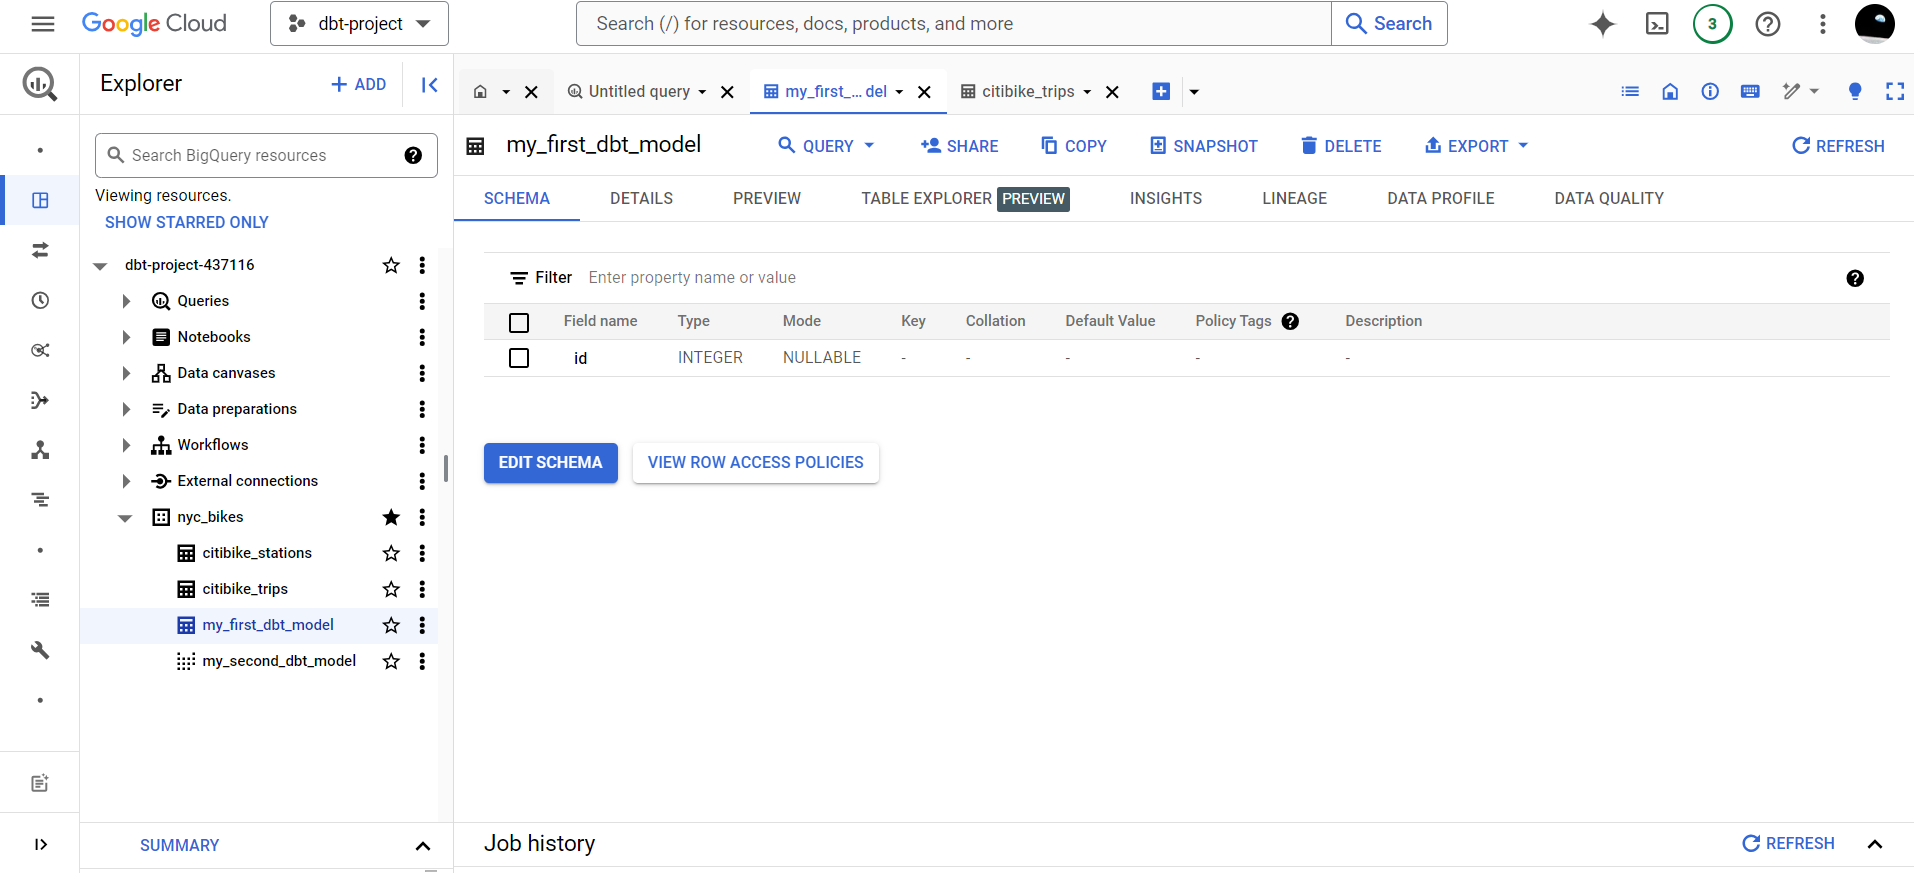
\includegraphics{./images/model_outputs.png}
\caption{Models}
\end{figure}

It was that simple, isn't it?

\hypertarget{model-structure}{%
\section{Model structure}\label{model-structure}}

Let's take a look at the model \texttt{my\_first\_dbt\_model.sql}.

\begin{verbatim}

{{ config(materialized='table') }}

with source_data as (

    select 1 as id
    union all
    select null as id

)

select *
from source_data

/*
    Uncomment the line below to remove records with null `id` values
*/

-- where id is not null
\end{verbatim}

The line \texttt{\{\{\ config(materialized=\textquotesingle{}table\textquotesingle{})\ \}\}} tells dbt to make the output \texttt{my\_first\_dbt\_model} as a table. Any configurations set at the model level will overide the overarching ones set at \texttt{dbt\_project.yml} file.

If you quickly take a sneek peek at the \texttt{dbt\_project.yml} file and scroll to the bottom, you will see this configuration:

\begin{verbatim}
models:
  dbt_book:
    # Config indicated by + and applies to all files under models/example/
    example:
      +materialized: view
\end{verbatim}

This configuration simply says that for every model inside the \texttt{dbt\_book/example} directory, materialize the result as a view\footnote{A view is a virtual table, similar to the original table, the physical dataset it was created from}. However, inside our \texttt{my\_first\_dbt\_model.sql} file, we set the materialization as \texttt{table}. What is in the sql model will override what is in the \texttt{dbt\_project.yml}. However, for \texttt{my\_second\_dbt\_model.sql}, we didn't specify the materialization. Therefore, by default, the materialization specified at the \texttt{dbt\_project.yml} level will be used.

\href{https://docs.getdbt.com/docs/build/materializations}{Materialization} is the persistence of a model in the data warehouse.

The second part of our first model is the actual SQL statement.

\begin{verbatim}
with source_data as (

    select 1 as id
    union all
    select null as id

)

select *
from source_data
\end{verbatim}

This is a \texttt{WITH} SQL statement. In very simple terms, the SQL statement in parentheses \texttt{()} is what is referenced as \texttt{source\_data}. Once we define our SQL statement and close it with parentheses, we can now select the data referenced by \texttt{source\_data}.

The SQL statements in parentheses is what is referred to as \href{https://www.atlassian.com/data/sql/using-common-table-expressions}{Common Table Expression (CTE)}. They were designed to simplify complex queries and be used in the context of a larger query.

The second model doesn't have much to provide but it introduces a new trick: the \texttt{ref} function.

\begin{verbatim}
select *
from {{ ref('my_first_dbt_model') }}
where id = 1
\end{verbatim}

The \texttt{ref} function is part of the jinja templating language. It is used to reference a model that has been provided within the parentheses and enclosed with quotes \texttt{(\textquotesingle{}\textquotesingle{})}. Therefore, in essence, our model simply returns the row(s) from \texttt{my\_first\_dbt\_model} that contain the value \texttt{1} in the \texttt{id} column.

Here is the result of \texttt{my\_second\_dbt\_model} view when I query BigQuery to show its contents.

\begin{figure}
\centering
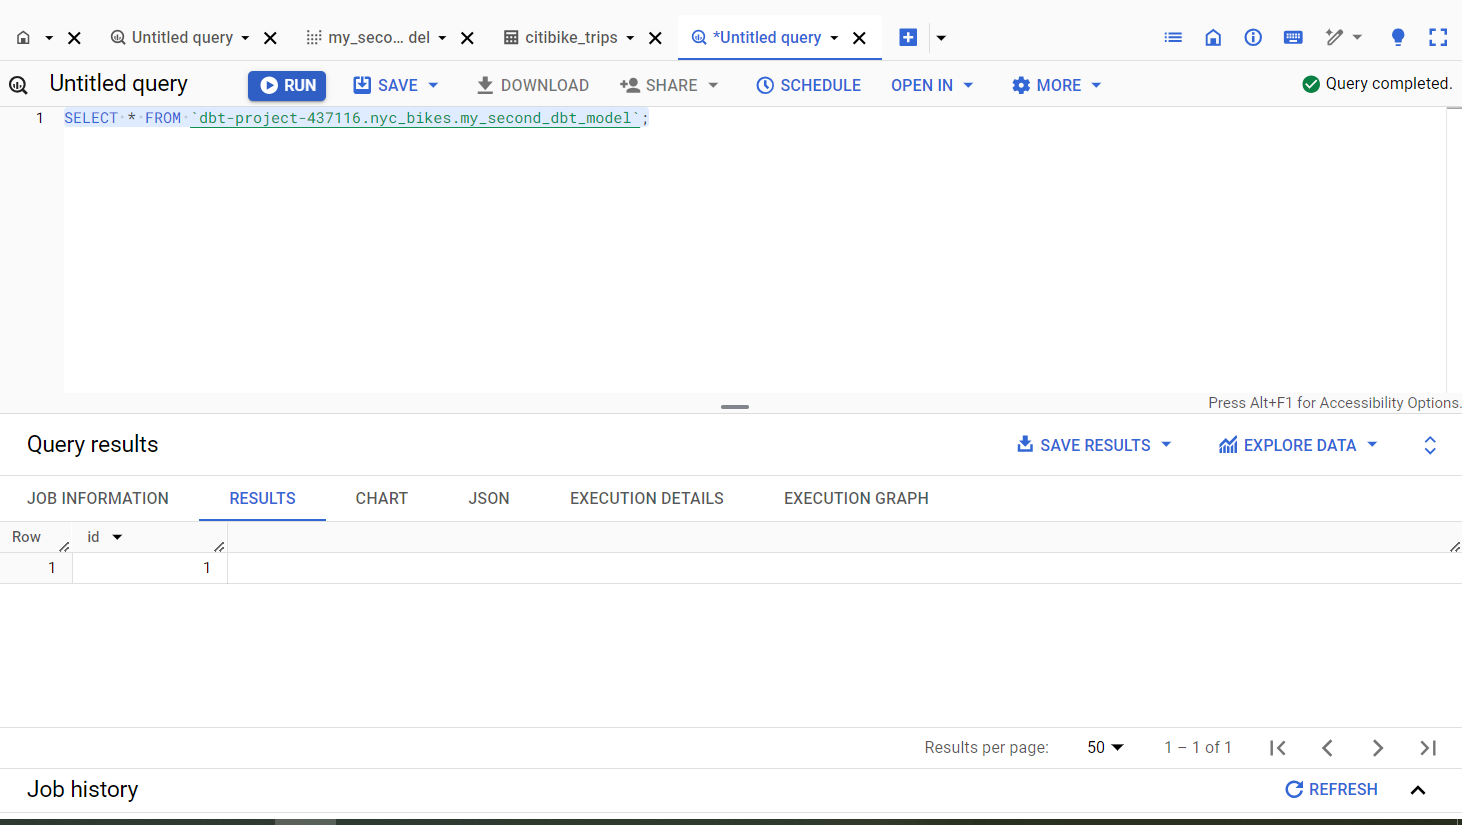
\includegraphics{./images/second_model.png}
\caption{Second model}
\end{figure}

\hypertarget{a-custom-model}{%
\section{A custom model}\label{a-custom-model}}

Now that we have seen how to run our models, it's now time to fold our shirts and run our own custom model.

Let's start easy. If you know SQL, there is no limit to the models, both in number and complexity, that you can do in dbt.

Our first model will endeavour to perform a change on the \texttt{citi\_trips} table within our \texttt{nyc\_bikes} dataset. In this dataset, there is a column called \texttt{tripduration} which shows the time in seconds for every cab trip. Humans prefer to read in minutes so a trivial dbt job would involve creating a column that shows the \texttt{tripduration} in minutes. By doing so, dbt would be performing the \textbf{T}ransform part in the ELT.

In the \texttt{citi\_trips\_minutes.sql} model, we have written a code that creates a view of this result. Remember, views are just virtual tables but they do save on storage!

\begin{verbatim}
{{ config(materialized='view') }}

WITH citi_trips AS (
    SELECT *, 
    tripduration / 60 AS trip_duration_min
    FROM 
    `dbt-project-437116.nyc_bikes.citibike_trips` 
)

SELECT * FROM citi_trips
\end{verbatim}

The above SQL statement is also a form of Common Table Expression (CTE). The variable \texttt{citi\_trips} just references the SQL statement in parentheses.

There is another small trick of the trade. What if this very simple dbt model was just part of thousands, and longer running SQL models? Would we have to run the entire lot of models? No.~To run only a specific model we use the \texttt{-\/-select} keyword.

Below we run the \texttt{citi\_trips\_minutes} model.

\begin{verbatim}
dbt run --select models/example/citi_trips_minutes.sql
\end{verbatim}

Below is the output.

\begin{verbatim}
Concurrency: 1 threads (target='dev')
18:50:33  
18:50:33  1 of 1 START sql view model nyc_bikes.citi_trips_minutes ....................... [RUN]
18:50:37  1 of 1 OK created sql view model nyc_bikes.citi_trips_minutes .................. [CREATE VIEW (0 processed) in 4.53s]
18:50:37  
18:50:37  Finished running 1 view model in 0 hours 0 minutes and 8.17 seconds (8.17s).
18:50:37  
18:50:37  Completed successfully
18:50:37  
18:50:37  Done. PASS=1 WARN=0 ERROR=0 SKIP=0 TOTAL=1
\end{verbatim}

We are always glad when we see the soothing words ``Completed successfully''. If you go to BigQuery, you will see a new view \texttt{citi\_trips\_minutes} already created. By default, the name of the newly formed view or table in the data warehouse will be that of the model used to create it.

Similar to the above, the below run command will also work. It doesn't have the file type (\texttt{.sql}) suffix.

\begin{verbatim}
dbt run --select citi_trips_minutes
\end{verbatim}

But how do we view this newly created result. Unlike a table, BigQuery does not offer the \textbf{PREVIEW} button. However, there is a way\ldots{}

\begin{figure}
\centering
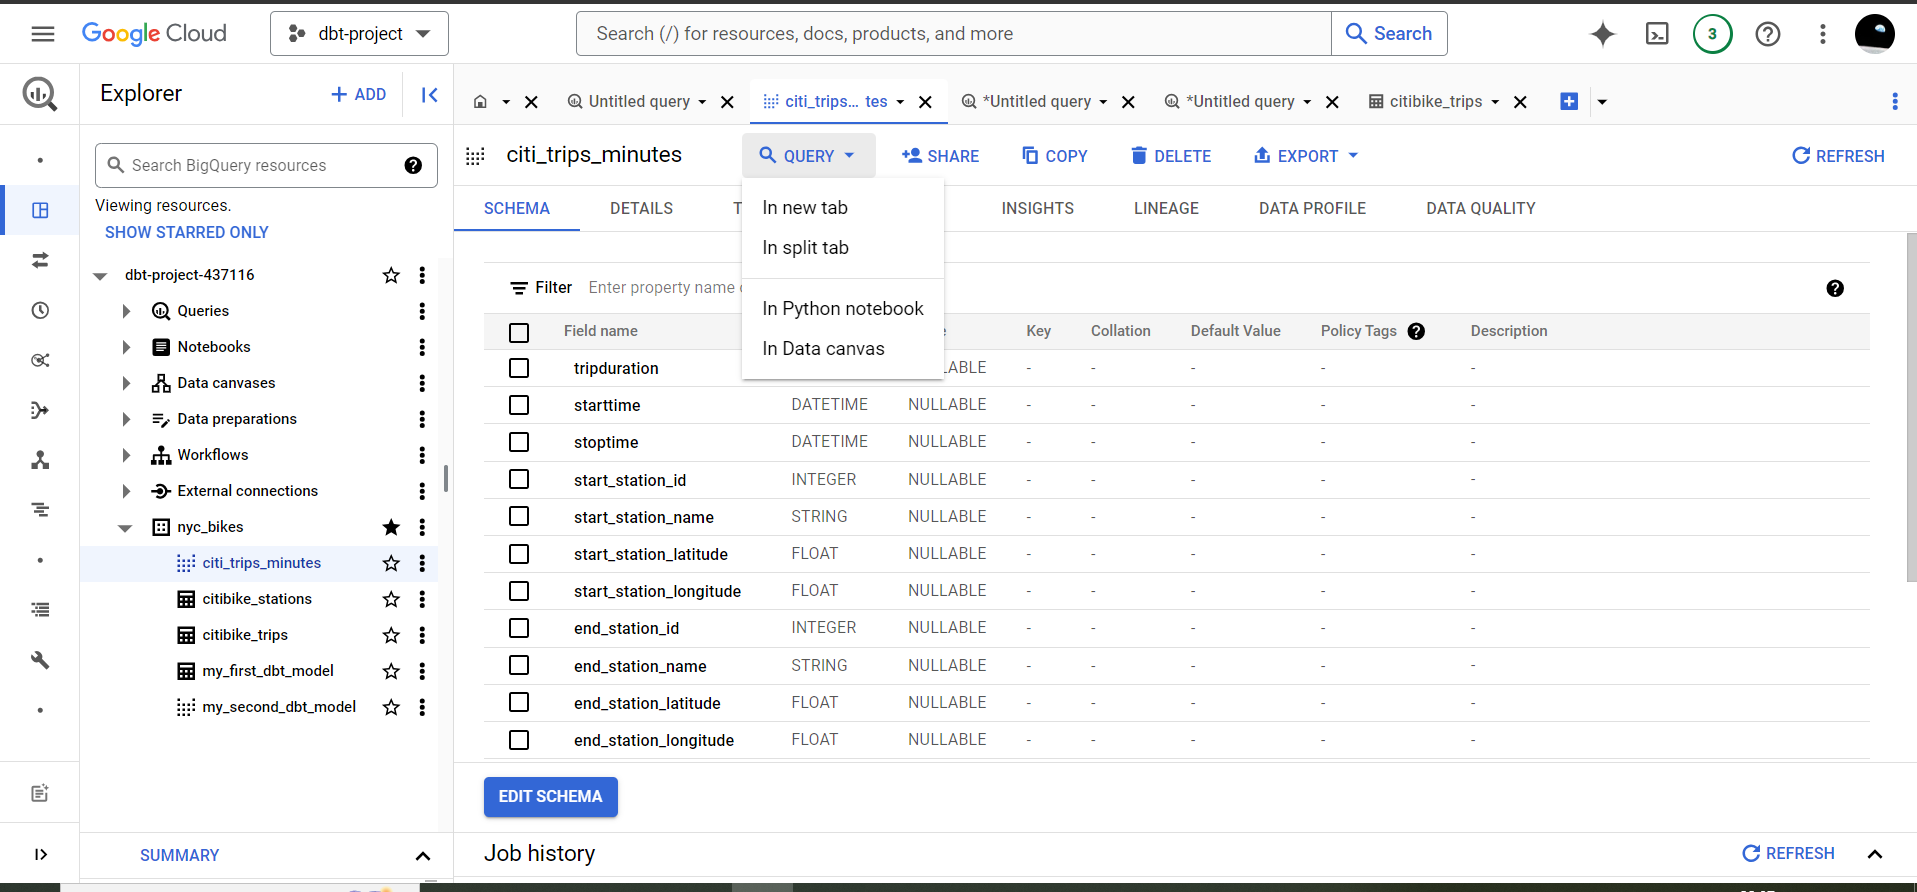
\includegraphics{./images/query_button.png}
\caption{Query}
\end{figure}

Click on the \textbf{Query} button, select \textbf{In new tab} and a new tab will form. Copy this SQL query onto the tab and run it to display the result of our \texttt{citi\_trips\_minutes} view.

\begin{verbatim}
SELECT * FROM `dbt-project-437116.nyc_bikes.citi_trips_minutes` 
\end{verbatim}

Our \texttt{trip\_duration\_min} column of interest is onto the far right of our view.

We had hinted earlier that there is no limit to the complexity or number of models you can create in dbt. Below is a more complex model. This model not only rounds off the minutes to one decimal place but also removes the null columns, thus reducing number of rows from 58,937,715 to 53,108,721. The model is saved as \texttt{citi\_trips\_round.sql}.

\begin{verbatim}
{{ config(materialized='view') }}

WITH citi_trips_round AS (
    SELECT *, ROUND(trip_duration_min, 1) AS trip_min_round
    FROM (
        SELECT *, 
        tripduration / 60 AS trip_duration_min
        FROM 
        `dbt-project-437116.nyc_bikes.citibike_trips`
        ) 
    WHERE tripduration IS NOT NULL
)

SELECT * FROM citi_trips_round
\end{verbatim}

Our model is saved as the \texttt{citi\_trips\_round} view in BigQuery.

Create a new query tab in BigQuery to view the results. Also use the query tab to count the number of rows and compare them to those from the \texttt{citibike\_trips} table. About 5.8 million rows with null value have been removed.

\begin{verbatim}
SELECT * FROM `dbt-project-437116.nyc_bikes.citi_trips_round`; 

SELECT COUNT(*) FROM `dbt-project-437116.nyc_bikes.citi_trips_round`;

-- This is the count of the original citibike_trips table
SELECT COUNT(*) FROM `dbt-project-437116.nyc_bikes.citibike_trips`;
\end{verbatim}

You may be wondering what's the advantage that dbt provides. After all, can't one just use the SQL Query tab in BigQuery just to do the transformations and save the table? Fine, that can work. However, dbt offers a form of persistence to your models. Though modifiable like those in BigQuery, they can be versioned when saved into a code versioning platform like Github.

One more thing, you don't have to use the \texttt{models/example} folder. You can choose to rename this one, or save the two models we created in a different folder. They will still run fine.

Create a new folder within the \texttt{models} directory called \texttt{my\_models}. Move the \texttt{citi\_trips\_minutes} and \texttt{citi\_trips\_round} models into the \texttt{my\_models} directory. Thereafter, run these two models using \texttt{dbt\ run\ -\/-select\ models/my\_models}. The models should run just fine.

As an extra bit of information, all successfully compiled and ran models will appear under the \texttt{/target} directory.

\hypertarget{documentation-1}{%
\chapter{Documentation}\label{documentation-1}}

In the book \emph{The voyages and adventures of Captain Hatteras} the sailors aboard a ship whose expedition was to the North Pole relied on the writing of former captains, explorers and sailsmen to not only find the best possible route to the North Pole, but also the hazards and the places where coal was hidden. So how does this tie to data engineering and dbt? Well, in any digital organization, there is sure to be some turnover. There is sure to be some new chap who would want to wrap their heads around what the organization was doing, and the data being used. Documentation is one way to enable these experts start on a sure footing, but this is rarely the norm. The good thing with dbt is that it provides a way to create documentation at the same place you write code to transform it, and not in a spare pdf\footnote{Portable Document Format}!

\hypertarget{the-yml-files}{%
\section{The yml files}\label{the-yml-files}}

In dbt, yml files can do a lot of things. One of the stuff it does is documentation and creation of tests for your data. But first, here are the rules of writing a yml file.

\begin{enumerate}
\def\labelenumi{\arabic{enumi}.}
\item
  Indents should be two spaces
\item
  List items should be indented
\item
  Use a new line to separate list items that are dictionaries where appropriate
\end{enumerate}

For this case, we shall use the YAML files to create documentation for our data. We already have a template to start us off with. This is the \texttt{schema.yml} file inside the \texttt{models/example} directory.

\begin{verbatim}
version: 2

models:
  - name: my_first_dbt_model
    description: "A starter dbt model"
    columns:
      - name: id
        description: "The primary key for this table"
        data_tests:
          - unique
          - not_null

  - name: my_second_dbt_model
    description: "A starter dbt model"
    columns:
      - name: id
        description: "The primary key for this table"
        data_tests:
          - unique
          - not_null
\end{verbatim}

Let's go through the above structure briefly.

\hypertarget{version-2}{%
\subsection{\texorpdfstring{\texttt{version:\ 2}}{version: 2}}\label{version-2}}

There is a story behind this. It is that at the very beginning of dbt development, the structure was very different and inserting \texttt{version:\ 2} enabled developers know which version of dbt they were working with. Don't expect a \texttt{version:\ 3} to come any time soon, but this is just a required necessity.

\hypertarget{models-2}{%
\subsection{\texorpdfstring{\texttt{models}}{models}}\label{models-2}}

Remember when we said that a model in dbt is simply a SQL file? Well, next to the \texttt{name} key which is under this key you specify the name of your SQL file, minus the \texttt{.sql} extension.

\hypertarget{description}{%
\subsection{\texorpdfstring{\texttt{description}}{description}}\label{description}}

This is where you insert the description of your table.

\hypertarget{columns}{%
\subsection{\texorpdfstring{\texttt{columns}}{columns}}\label{columns}}

These are the fields contained in your table. You name them here and under each column are three mappings.

\begin{itemize}
\item
  \texttt{name} - this is the name of the field in your table. In other words, it is the column name.
\item
  \texttt{description} - this is a short explanation of your column.
\item
  \texttt{data\_test} - the kind of tests that you would like to perform on your field are inserted here. dbt comes with generic tests such as \texttt{unique}, \texttt{not\_null} and \texttt{integer} but you can create your own custom tests too.
\end{itemize}

\hypertarget{definition-for-our-model}{%
\section{Definition for our model}\label{definition-for-our-model}}

Alright, having gone through the template, we can create our own \texttt{yml} file under the \texttt{my\_models} directory. Let's call it \texttt{my\_models.yml}. Copy past the YAML structure from \texttt{schema.yml} to the \texttt{my\_models.yml} and let the first YAML structure for \texttt{citi\_trips\_minutes.sql} look like below.

\begin{verbatim}
version: 2

models:
  - name: citi_trips_minutes
    description: "This is a table with an extra column showing the trip duration in minutes"
    columns:
      - name: tripduration
        description: "Trip Duration (in seconds)"

      - name: starttime
        description: "Start Time, in NYC local time."
      
      - name: stoptime
        description: "Stop Time, in NYC local time."

      - name: start_station_id
        description: "Start Station ID"
      
      - name: start_station_name
        description: "Start Station Name"

      - name: start_station_latitude
        description: "Start Station Latitude"
      
      - name: start_station_longitude
        description: "Start Station Longitude"

      - name: end_station_id
        description: "End Station ID"

      - name: end_station_name
        description: "End Station Name"

      - name: end_station_latitude
        description: "End Station Latitude"

      - name: end_station_longitude
        description: "End Station Longitude"
      
      - name: bike_id
        description: "Bike ID"
      
      - name: usertype
        description: "User Type (Customer = 24-hour pass or 7-day pass user, Subscriber = Annual Member)"

      - name: birth_year
        description: "Year of Birth"

      - name: gender
        description: "Gender (unknown, male, female)"

      - name: customer_plan
        description: "The name of the plan that determines the rate charged for the trip"

      - name: trip_duration_min
        description: "The trip duration in minutes"
\end{verbatim}

What we've done is quite straightforward. We have simply typed out the descriptions next to the \texttt{description} mapping key.

However, imagine you were working with hundreds of models which use similar definitions. Would you have the nerve to copy paste every definition to its respective model? Perhaps not. There is a function by the name of the \texttt{docs()} function which can reference to descriptions in a separate markdown file.

\hypertarget{using-the-doc-function}{%
\section{\texorpdfstring{Using the \texttt{doc} function}{Using the doc function}}\label{using-the-doc-function}}

To use the \texttt{doc()} function, we write our definitions in a separate markdown \texttt{(.md)} file and place the descriptions within \texttt{\{\%\ docs\ \textless{}field-name\textgreater{}\ \%\}} \texttt{\{\%\ enddocs\ \%\}} tags. For this tutorial, we created three markdown tables.

\begin{itemize}
\item
  \texttt{references.md} - this contains the descriptions for our column names of interest
\item
  \texttt{tables.md} - contains the descriptions for our tables of interest
\item
  \texttt{overview.md} - contains the text that will go to the overview page
\end{itemize}

Here is what our \texttt{references.md} contains. As you can see, we have provided some textual information for some of our column names. We can also add some more style to our descriptions since they are now on a separate markdown. For example we could insert links, make the text italic, and bold if you wish!

\begin{verbatim}


Trip Duration (in seconds). Like:

- How long did the trip take?
- What is the time in seconds?
- More info on time, see [here](https://www.poemhunter.com/poem/time-xxi/)

*https://www.poemhunter.com/poem/time-xxi/*





Start Time, in NYC local time. As accurate as could ever be.



--snip--
\end{verbatim}

The \texttt{tables.md} just contains a description of our \texttt{citi\_trips\_round} table.

\begin{verbatim}


This table contains the trip duration in minutes to one decimal place only. 


\end{verbatim}

Now, in order to enable dbt reference these descriptions from our YAML file, we would simply use the \texttt{doc\ ()} function as shown below:

\begin{verbatim}
- name: citi_trips_round
    description: '{{ doc("citi_trips_round") }}'
    columns:
      - name: tripduration
        description: '{{ doc("tripduration") }}'

      - name: starttime
        description: '{{ doc("starttime") }}'
      
      - name: stoptime
        description: '{{ doc("stoptime") }}'

      - name: start_station_id
        description: "Start Station ID"
        
--snip--
\end{verbatim}

The file saved as \texttt{overview.md} in our project will be used to display the home page of our dbt documentation website. However, the homepage uses a different syntax, like so:

\begin{verbatim}


Some more text here...


\end{verbatim}

Therefore, here is some dummy text for our overview page.

\begin{verbatim}


# Learning dbt

Learning is not merely the acquisition of knowledge, but the cultivation of the mind. It is through the active engagement of our intellect that we develop the capacity for critical thought, discernment, and wisdom. 

--snip--


\end{verbatim}

\hypertarget{images-in-dbt-documentation}{%
\section{Images in dbt documentation}\label{images-in-dbt-documentation}}

They say an image is worth a thousand words. In dbt, we store images in a folder called \texttt{assets}. Ideally, one can create any folder in dbt to store images provided you reference it correctly in the documentation. However, for versioning purposes, it is better you store it in an \texttt{assets} folder. Furthermore, images in dbt, once run as part of your document generation, will also appear under the \texttt{targets/} folder just like your SQL models.

Therefore, going with the recommended approach, create an \texttt{assets/} folder under \texttt{dbt\_book}. Place your image in there.

Go to the \texttt{dbt\_projects.yml} file and create a new line with the following code:

\begin{verbatim}
asset-paths: ["assets"]
\end{verbatim}

This path tells dbt to copy all items within \texttt{assets} into the \texttt{target} directory. Any image in a different directory will not get copied into the \texttt{target} directory when documents are generated.

Finally, as the missing piece to the puzzle, insert a reference to your image in the \texttt{overview.md} file.

\begin{verbatim}
![Example image](assets/image_example.jpg)
\end{verbatim}

One can also create \href{https://docs.getdbt.com/docs/build/documentation\#setting-a-custom-overview}{custom overviews} for the dbt packages they used.

Below is our complete \texttt{overview.md} file.

\begin{verbatim}


# Learning dbt

Learning is not merely the acquisition of knowledge, but the cultivation of the mind. It is through the active engagement of our intellect that we develop the capacity for critical thought, discernment, and wisdom. By examining the world around us with curiosity and rigor, we uncover the underlying principles that govern its workings. This intellectual pursuit not only broadens our understanding but also equips us to navigate life's challenges with greater clarity and purpose.

![Example image](assets/image_example.jpg)

Some more text here...


\end{verbatim}

\hypertarget{generating-the-document}{%
\section{Generating the document}\label{generating-the-document}}

Now is the time where we ignite the rocket engines and shoot off. To generate a dbt documentation, first run \texttt{dbt\ docs\ generate}. This command tells dbt to compile the necessary information of your project into the \texttt{catalog.json} and \texttt{manifest.json} files. The ignition key for our documentation generation is \texttt{dbt\ docs\ serve}. dbt will generate a list of outputs and create a popup providing the link to open up your documentation. You can click on the popup or copy-paste the link. Our documentation is in the host: \texttt{localhost:8080/}.

\begin{figure}
\centering
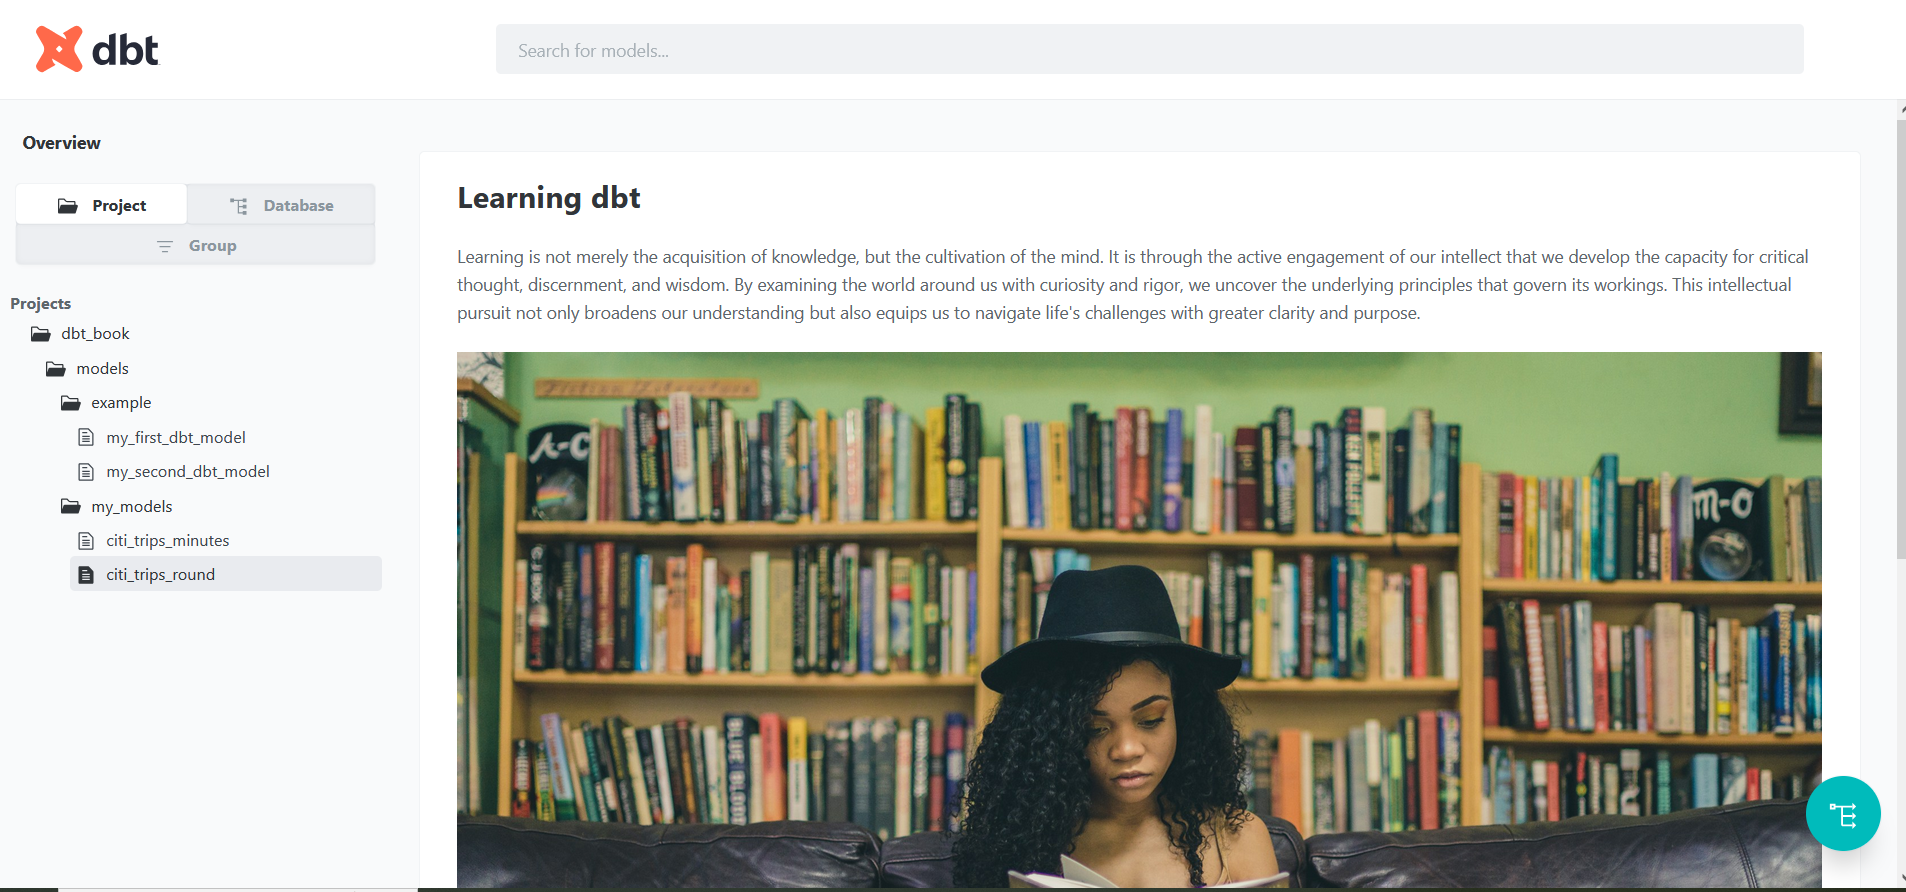
\includegraphics{./images/overview_page.png}
\caption{Model page}
\end{figure}

\begin{figure}
\centering
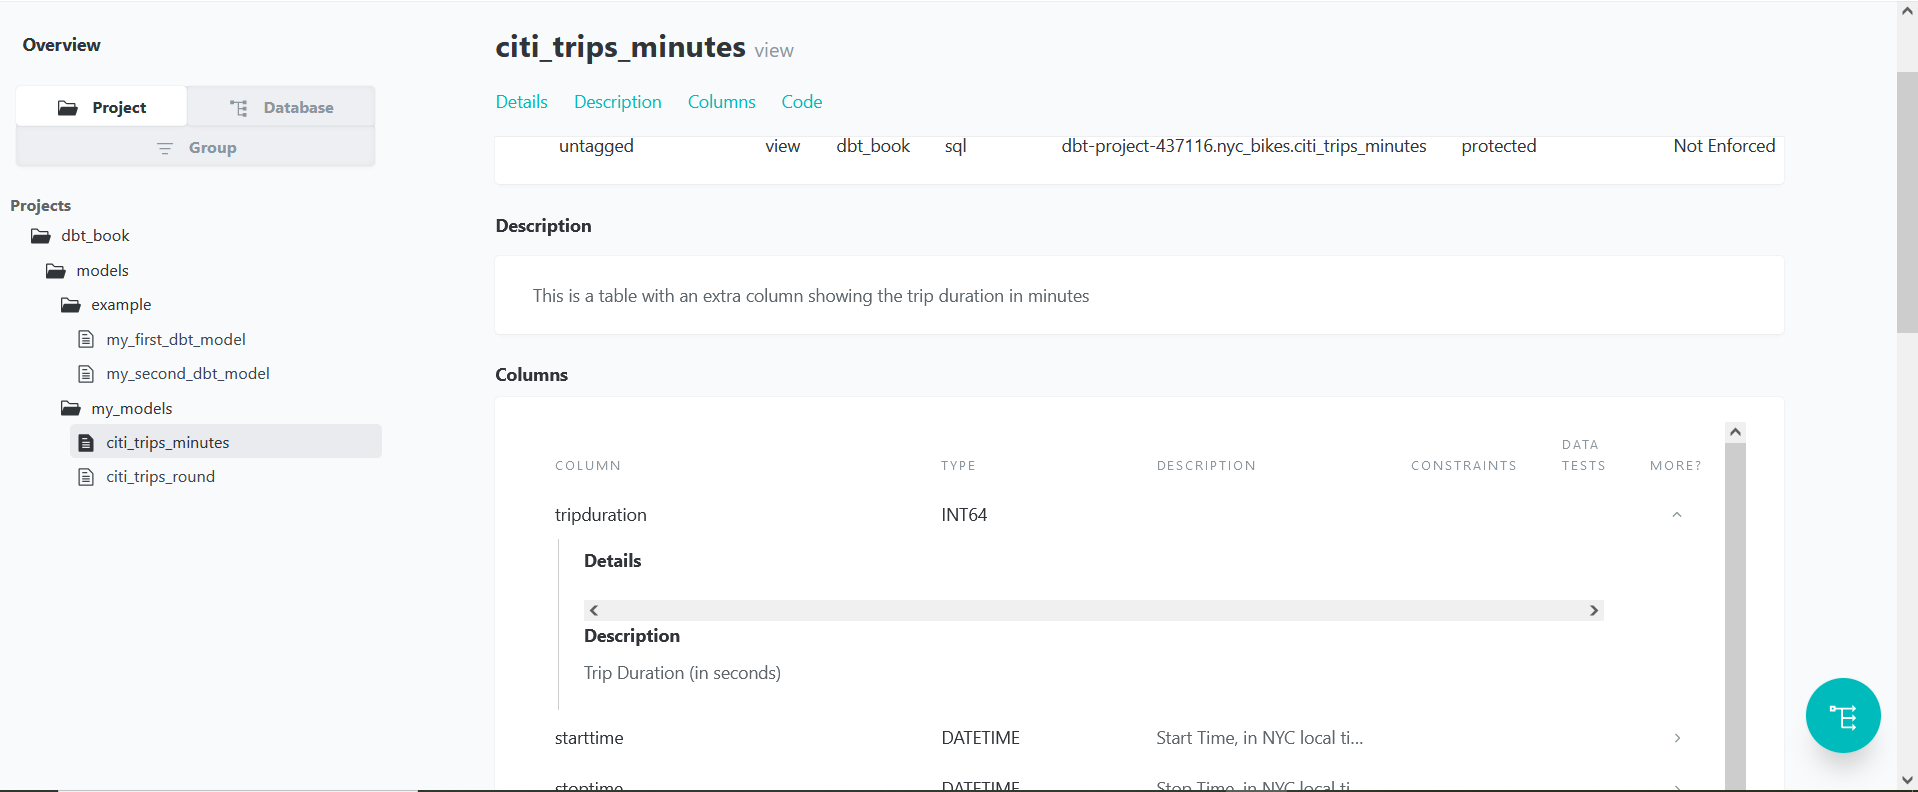
\includegraphics{./images/model_page.png}
\caption{Models page}
\end{figure}

If you go to the \texttt{targets} directory, our image(s) will be there!

There is also one more cool functionality of the dbt documentation. On the bottom right, there is a turquoise button for showing the lineage graph for each model. If you click on any model, such as \texttt{my\_second\_dbt\_model}, you will see it shows a dependency on \texttt{my\_first\_dbt\_model}. If you have worked on a model that has several dependencies, or children, the model will most likely be more complex. A good example will be for the \texttt{citi\_trips\_long} model.

\begin{figure}
\centering
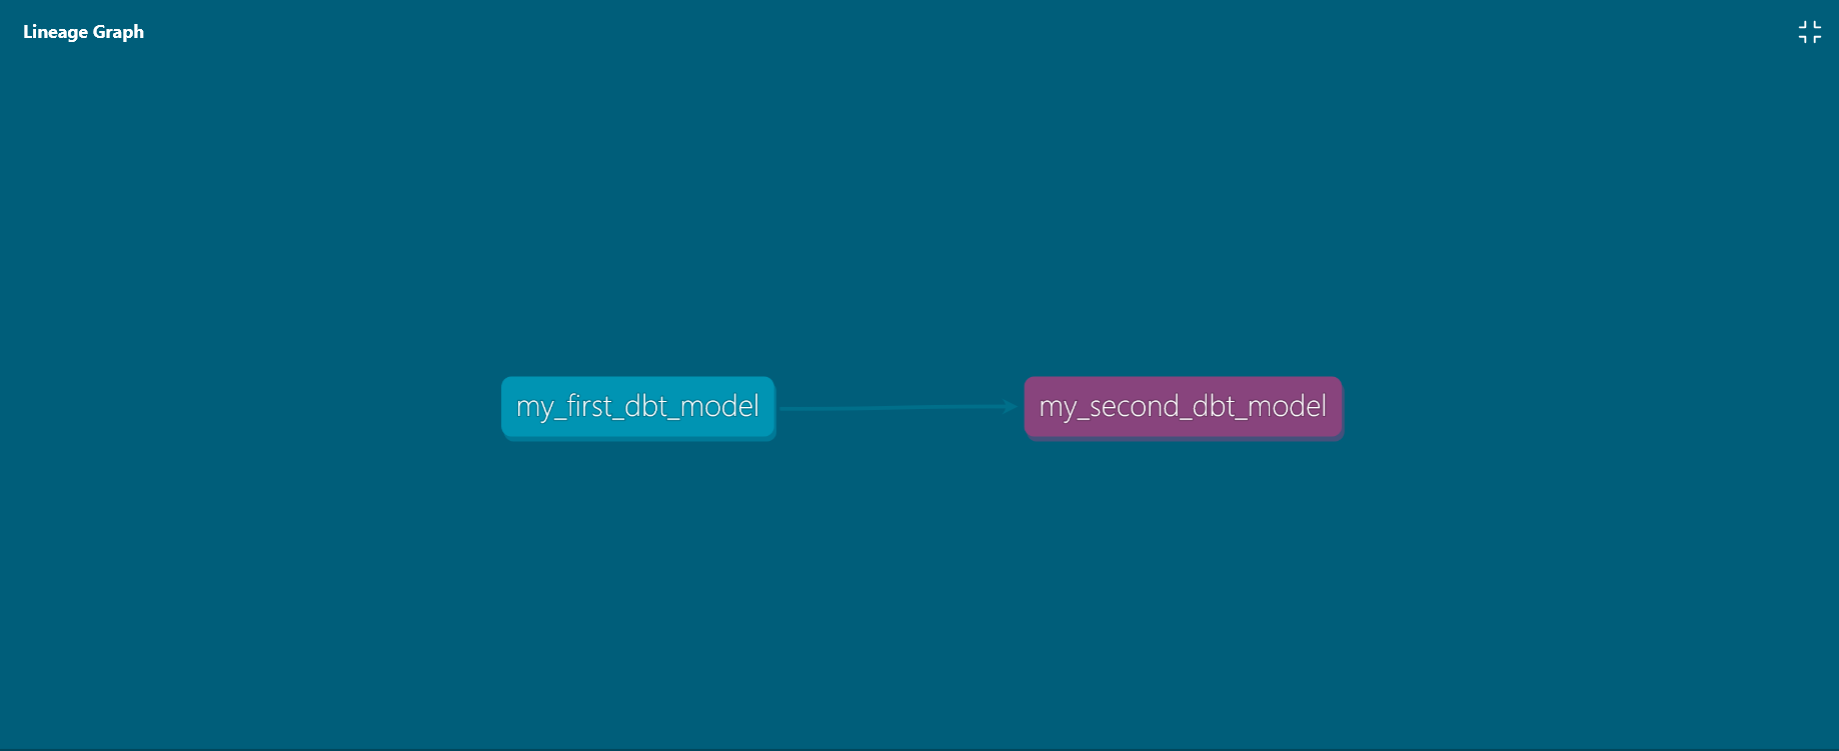
\includegraphics{./images/lineage_graph.png}
\caption{Lineage graph}
\end{figure}

It is highly encouraged to play around with the buttons \textbf{resources}, \textbf{packages}, \textbf{tags}, \textbf{--select} and \textbf{--exclude}. For the \textbf{select} button, play around with inserting \texttt{+} both before and after the name of the model. Clue: it has to do with showing or hiding the model's dependencies and/or children.

Below is an example of the \texttt{citi\_trips\_long} model, which has more than one dependency.

\begin{figure}
\centering
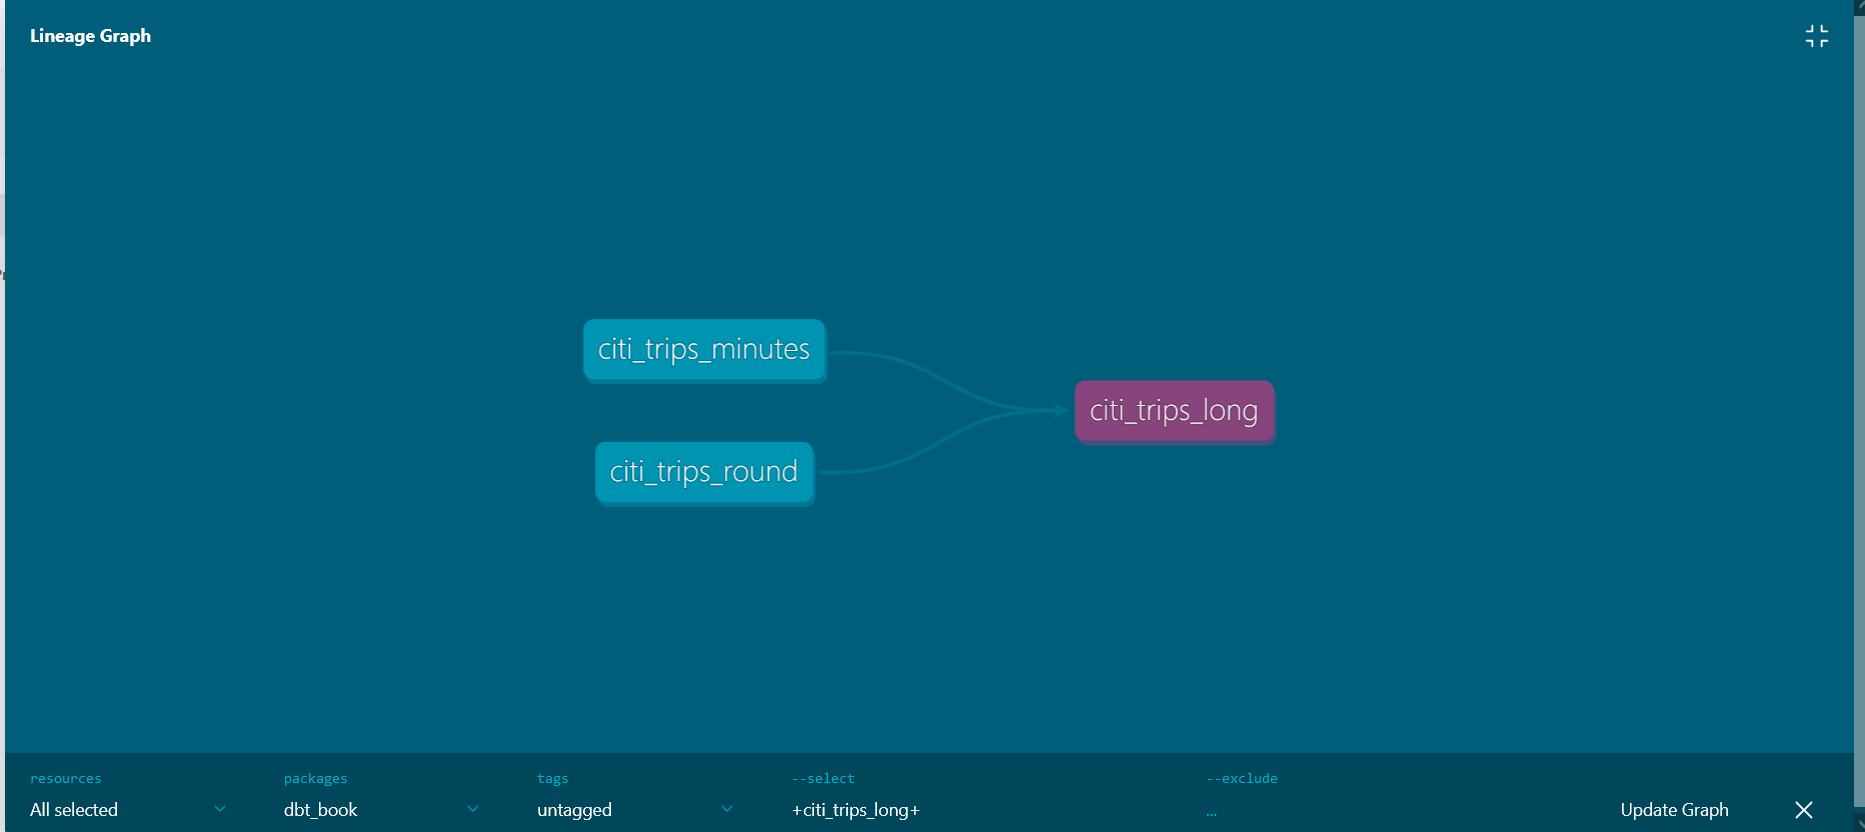
\includegraphics{./images/lineage_graph2.png}
\caption{A model with more than one dependency}
\end{figure}

\hypertarget{tests-1}{%
\chapter{Tests}\label{tests-1}}

Probably if you've worked on a Windows computer, you must have used Microsoft Defender Full Scan at some point. During or at the end of the scan, some results were displayed. dbt works in almost the same way, only that this time they scan your data.

Tests in dbt are basically assertions of your data. That is, they are just some assumptions that you have of your datasets that are correct. Tests enable one to know: 1) which assumptions are wrong about our data, and 2) which parts of our data diverge from the expected norm. Tests can sometimes feel like something to bemoan, can fail (as all tests do) but the overarching advantage is that they make us understand more about our data. They can also be lifesavers in that they can pinpoint a serious problem which could be harder to debug later on! In a nutshell, dbt tests perform much like a programmatic scan that will only spew out errors of something that is suspicious.

\hypertarget{types-of-tests-in-dbt}{%
\section{Types of tests in dbt}\label{types-of-tests-in-dbt}}

In dbt, a test can be defined in either of the following two ways:

\begin{enumerate}
\def\labelenumi{\arabic{enumi}.}
\tightlist
\item
  generic test - this is a test written in a SQL model and defined inside a YAML file. The test in the YAML file is defined using jinja Macros. dbt comes with four all-batteries included tests namely:
\end{enumerate}

\begin{itemize}
\tightlist
\item
  unique - asserts that the column has no repeating values
\item
  not\_null - asserts that there are no null values
\item
  accepted\_values - checks if the values in your field correspond to those in a defined list
\item
  relationships - checks if the field has an existing relationship with another field in a different table.
\end{itemize}

\begin{enumerate}
\def\labelenumi{\arabic{enumi}.}
\setcounter{enumi}{1}
\tightlist
\item
  singular test - some normally refer to this as a custom test. This is a SQL query which is used to check assertions in your data. The SQL files that make up your test are defined inside the \texttt{tests} directory or the path defined in the \texttt{test-paths} key inside the \texttt{dbt\_project.yml} file. Each SQL file will have one test only. Nevertheless, if this test will be used across many fields and files, you can reference it using jinja macros \texttt{\{\{\ \}\}}. If this is the case, it is no longer a singular test but a generic \emph{custom} test.
\end{enumerate}

Let's start with a dbt out-of-the-box generic test.

\hypertarget{generic-tests-in-dbt}{%
\section{Generic tests in dbt}\label{generic-tests-in-dbt}}

We will start with a very simple test, the \texttt{not\_null} test on the \texttt{start\_station\_name} column of \texttt{citi\_trips\_long} model. Surely, unless someone is teleporting from somewhere, every rented bike must have an origin.

\begin{verbatim}

- name: citi_trips_long
    description: '{{ doc("citi_trips_long") }}'
    columns:
      - name: starttime
        description: '{{ doc("starttime") }}'

      --snip--

      - name: start_station_name
        description: "Start Station Name"
        tests:
          - not_null
          
\end{verbatim}

We use the below code to test only those models under \texttt{my\_models} folder.

\begin{verbatim}
dbt test --select my_models
\end{verbatim}

Here is the output.

\begin{verbatim}
--snip--

19:15:33  Concurrency: 1 threads (target='dev')
19:15:33  
19:15:33  1 of 1 START test not_null_citi_trips_long_start_station_name .................. [RUN]
19:15:36  1 of 1 PASS not_null_citi_trips_long_start_station_name ........................ [PASS in 3.20s]
19:15:36  
19:15:36  Finished running 1 test in 0 hours 0 minutes and 4.44 seconds (4.44s).
19:15:36  
19:15:36  Completed successfully
19:15:36  
19:15:36  Done. PASS=1 WARN=0 ERROR=0 SKIP=0 TOTAL=1
\end{verbatim}

If we had gone with the more blanket code of \texttt{dbt\ test}, it would have also tested those models under the shipped \texttt{examples} folder where there is already a test designed to fail, purely for demonstration purposes. Back to our \texttt{citi\_trips\_long} model, we can see that the test passed successfully. As expected, there are no null values in our \texttt{start\_station\_name} field. If the opposite happened, then there must be a row with a null value under this field.

Now let's create a test that will fail on purpose. From a large dataset, obviously the station names can't be unique all through. So we insert the \texttt{unique} value under the \texttt{tests} key as follows:

\begin{verbatim}
- name: start_station_name
        description: "Start Station Name"
        tests:
          - not_null
          - unique
\end{verbatim}

The output is as below. Note that it results in a failure and also shows the path to the SQL query inside the \texttt{target/} directory that was used to carry out the test. If you paste this SQL query from the \texttt{target} directory into your data warehouse, it will return the number of rows that failed the test.

\begin{verbatim}
19:23:35  Concurrency: 1 threads (target='dev')
19:23:35  
19:23:35  1 of 2 START test not_null_citi_trips_long_start_station_name .................. [RUN]
19:23:38  1 of 2 PASS not_null_citi_trips_long_start_station_name ........................ [PASS in 3.01s]
19:23:38  2 of 2 START test unique_citi_trips_long_start_station_name .................... [RUN]
19:23:41  2 of 2 FAIL 910 unique_citi_trips_long_start_station_name ...................... [FAIL 910 in 2.68s]
19:23:41  
19:23:41  Finished running 2 data tests in 0 hours 0 minutes and 6.78 seconds (6.78s).
19:23:41  
19:23:41  Completed with 1 error and 0 warnings:
19:23:41  
19:23:41  Failure in test unique_citi_trips_long_start_station_name (models/my_models/my_models.yml)
19:23:41    Got 910 results, configured to fail if != 0
19:23:41  
19:23:41    compiled code at target/compiled/dbt_book/models/my_models/my_models.yml/unique_citi_trips_long_start_station_name.sql
19:23:41  
19:23:41  Done. PASS=1 WARN=0 ERROR=1 SKIP=0 TOTAL=2
\end{verbatim}

\begin{figure}
\centering
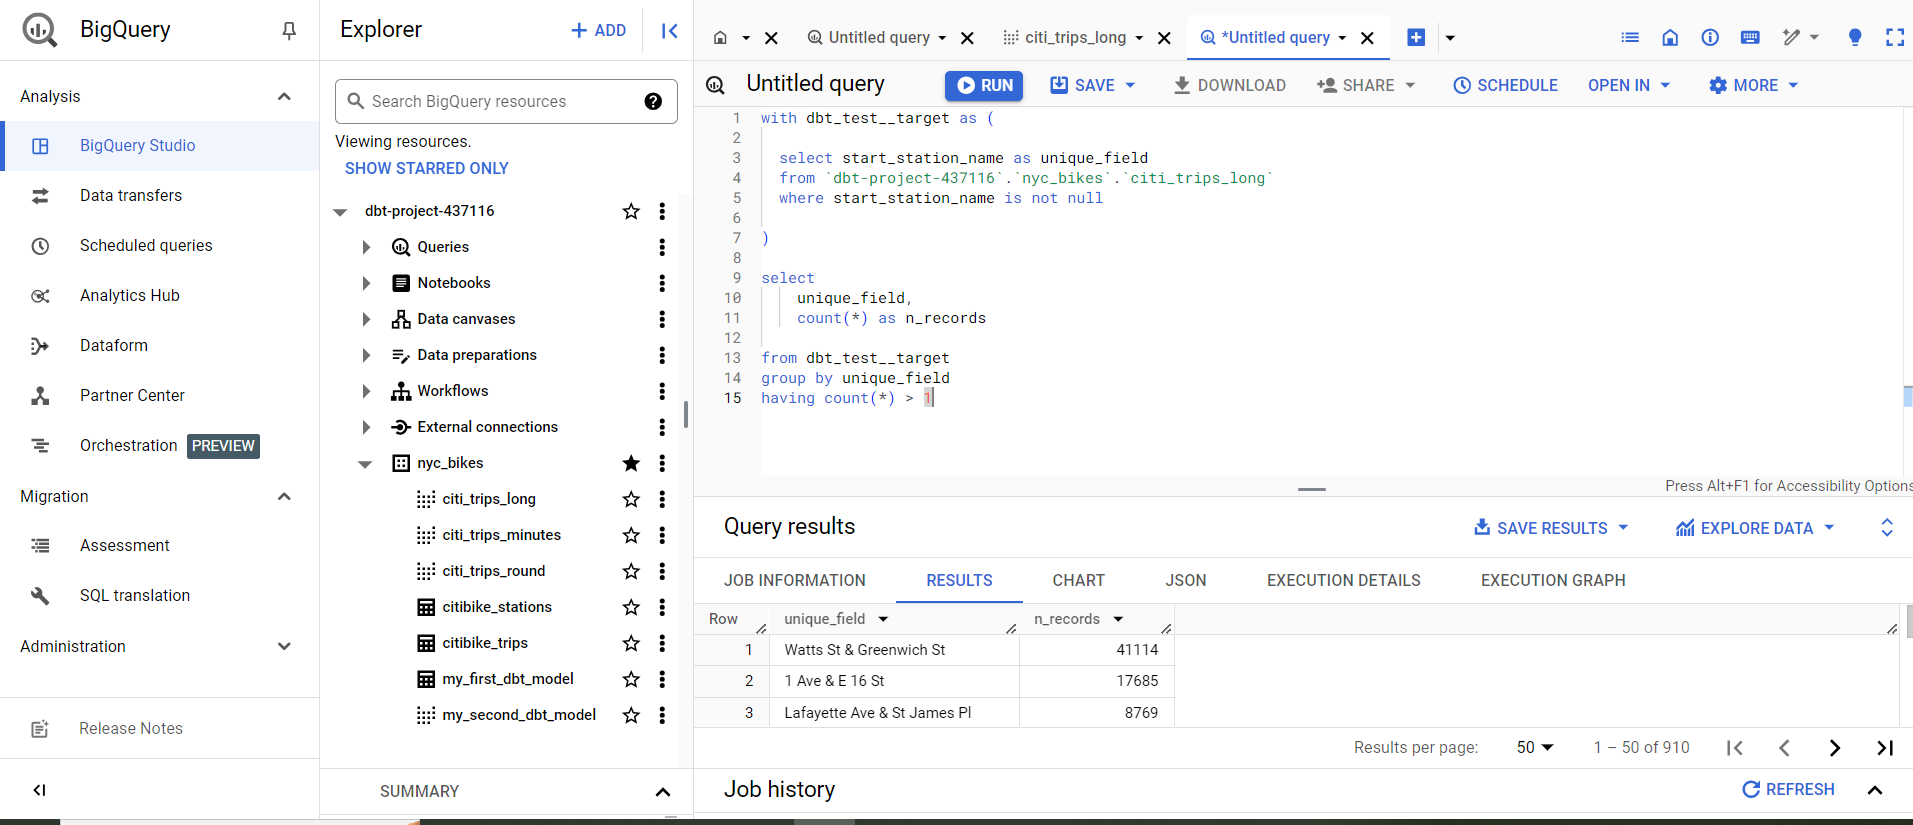
\includegraphics{./images/failed_test.png}
\caption{Failed test}
\end{figure}

\hypertarget{singular-tests-in-dbt}{%
\section{Singular tests in dbt}\label{singular-tests-in-dbt}}

As mentioned earlier, singular tests are SQL models in your \texttt{tests} folder. They differ from the generic tests in that they are bespoke to your data needs. For example, if one of your tests doesn't conform to the four tests shipped with dbt, you can create one inside the \texttt{tests} folder.

Below we create a singular test called \texttt{unnecessary\_trips.sql} inside the \texttt{test} folder. The purpose of the test is to raise an error if a trip is less than 10 min. The latter must surely generate an error! Notice that one can reference another model within a test using the \texttt{ref()} function.

\begin{verbatim}
SELECT bikeid, start_station_name, end_station_name,
    birth_year, gender, tripduration
FROM {{ ref('citi_trips_round') }}
WHERE trip_min_round < 10
\end{verbatim}

So to perform the litmus test, run our usual magic phrase:

\begin{verbatim}
dbt test --select unnecessary_trips
\end{verbatim}

Below will be the output.

\begin{verbatim}
19:51:50  Concurrency: 1 threads (target='dev')
19:51:50  
19:51:50  1 of 1 START test unnecessary_trips ............................................ [RUN]
19:51:53  1 of 1 FAIL 25183763 unnecessary_trips ......................................... [FAIL 25183763 in 3.11s]
19:51:53  
19:51:53  Finished running 1 test in 0 hours 0 minutes and 4.70 seconds (4.70s).
19:51:53  
19:51:53  Completed with 1 error and 0 warnings:
19:51:53  
19:51:53  Failure in test unnecessary_trips (tests/unnecessary_trips.sql)
19:51:53    Got 25183763 results, configured to fail if != 0
19:51:53  
19:51:53    compiled code at target/compiled/dbt_book/tests/unnecessary_trips.sql
19:51:53  
19:51:53  Done. PASS=0 WARN=0 ERROR=1 SKIP=0 TOTAL=1
\end{verbatim}

As you can see, a total 25183763 rows failed the test.

A singular test can also be transformed into a generic test when its reused across the fields of your table(s) in the data warehouse. To demonstrate this, let's create some generic tests.

\hypertarget{creating-a-generic-test}{%
\section{Creating a generic test}\label{creating-a-generic-test}}

\emph{Custom} generic tests are created within a \texttt{generic} folder within the \texttt{tests} directory. Thus, within your \texttt{tests/generic} directory, you will place the SQL models for your tests. Anything returned by your SQL models is in fact your tests failing! If nothing is returned, then your test passed!

Create a SQL model called \texttt{long\_characters} within the \texttt{tests/generic} directory.

\begin{verbatim}

SELECT * FROM {{ model }}
WHERE LENGTH({{ column_name }}) > 15 

\end{verbatim}

Let's go through the above query line by line. We begin a generic test by using the \texttt{\{\%test\ \textless{}model-name\textgreater{}\ (model,\ column\_name)\ \%\}} \emph{SQL statement in here} \texttt{\{\%\ endtest\ \%\}} tags. The \texttt{model} and \texttt{column\_name} are standard arguments where one or both should be defined.

\begin{itemize}
\item
  \texttt{model} - the resource on which the test will be operated on. In our case, this is any model which the test will run on.
\item
  \texttt{column\_name} - this is a field within which the model will be run against. In other words, the column at which this model will operate on.
\end{itemize}

The SQL statement within the test tags references the model and the columns using the \texttt{\{\{\ model\ \}\}} and \texttt{\{\{\ column\_name\ \}\}} respectively. For example, if the test is placed in the \texttt{my\_models} YAML file, under the \texttt{citi\_trips\_long} model name, for the field \texttt{start\_station\_name}, it is as though the test is running this SELECT statement:

\begin{verbatim}
SELECT * FROM citi_trips_long
WHERE LENGTH(start_station_name) > 15 
\end{verbatim}

In very few words, the above SQL tells dbt to shout out an error if any station name is greater than 15 characters.

Let's create another test that will raise alarms if there are special characters within your \texttt{start\_station\_name}.

\begin{verbatim}

SELECT * FROM {{ model }}
WHERE {{ column_name }}
LIKE '%^[a-zA-Z0-9+-]%'

\end{verbatim}

Okay, it's now time for our litmus test. Going back to the \texttt{start\_station\_name} mapping that we have performed some litmus tests, lets also add our two \emph{custom} generic tests of \texttt{long\_character} and \texttt{special\_characters}.

\begin{verbatim}
- name: citi_trips_long
    description: '{{ doc("citi_trips_long") }}'
    columns:
      --snip--

      - name: start_station_name
        description: "Start Station Name"
        tests:
          - not_null
          - unique
          - long_characters
          - special_characters
\end{verbatim}

If we go for the big bull and run all our tests with the trusty \texttt{dbt\ test} keyword, we can see the output of the nine tests we have so far.

\begin{verbatim}
19:08:15  Concurrency: 1 threads (target='dev')
19:08:15  
19:08:15  1 of 9 START test long_characters_citi_trips_long_start_station_name ........... [RUN]
19:08:29  1 of 9 FAIL 11463868 long_characters_citi_trips_long_start_station_name ........ [FAIL 11463868 in 14.47s]

--snip--

19:08:55  5 of 9 START test special_characters_citi_trips_long_start_station_name ........ [RUN]
19:08:59  5 of 9 PASS special_characters_citi_trips_long_start_station_name .............. [PASS in 4.48s]

--snip--

19:09:07  9 of 9 START test unnecessary_trips ............................................ [RUN]
19:09:10  9 of 9 FAIL 25183763 unnecessary_trips ......................................... [FAIL 25183763 in 2.81s]
\end{verbatim}

From the above output, we can see that there were some station names with quite some long names and (thankfully) no station names with special characters.

There is also another output following the above which shows how many records failed, depending on your test.

\begin{verbatim}
19:09:10  Completed with 4 errors and 0 warnings:
19:09:10  
19:09:10  Failure in test long_characters_citi_trips_long_start_station_name (models/my_models/my_models.yml)
19:09:10    Got 11463868 results, configured to fail if != 0
 
--snip--

19:09:10  Failure in test unique_citi_trips_long_start_station_name (models/my_models/my_models.yml)
19:09:10    Got 910 results, configured to fail if != 0
\end{verbatim}

\hypertarget{configuring-custom-generic-tests}{%
\section{Configuring custom generic tests}\label{configuring-custom-generic-tests}}

What if you feel that the \emph{FAIL} alert like in the above tests is shouting too much?! That you would prefer them to be \emph{WARNINGS} because they are non-critical?

You can do so by setting the configuration to display as a warning rather than an error.

\begin{verbatim}

    {{ config(severity = 'warn') }}
    SELECT * FROM {{ model }}
    WHERE LENGTH({{ column_name }}) > 15 

\end{verbatim}

Here is the output as a warning.

\begin{verbatim}

19:16:34  1 of 9 START test long_characters_citi_trips_long_start_station_name ........... [RUN]
19:16:36  1 of 9 WARN 11463868 long_characters_citi_trips_long_start_station_name ........ [WARN 11463868 in 2.64s]
19:16:36  2 of 9 START test not_null_citi_trips_long_start_station_name .................. [RUN]
19:16:39  2 of 9 PASS not_null_citi_trips_long_start_station_name ........................ [PASS in 2.67s]
-- snip --
19:16:56  Warning in test long_characters_citi_trips_long_start_station_name (models/my_models/my_models.yml)
19:16:56  Got 11463868 results, configured to warn if != 0
-- snip --
\end{verbatim}

However, in case you immediately change your mind that the failing tests of \texttt{long\_characters} should be an error rather than a warning, you can override your custom generic SQL models by specifying the severity within the YAML definition files.

\begin{verbatim}
- name: start_station_name
        description: "Start Station Name"
        tests:
          - not_null
          - unique
          - long_characters:
            severity: 'error'
          - special_characters
\end{verbatim}

In the generated output, it will be back to business as usual with the `FAIL' keyword.

\begin{verbatim}
-- snip -- 
19:21:25  1 of 9 START test long_characters_citi_trips_long_start_station_name ........... [RUN]
19:21:28  1 of 9 FAIL 11463868 long_characters_citi_trips_long_start_station_name ........ [FAIL 11463868 in 3.45s]
-- snip --

19:21:50  Failure in test long_characters_citi_trips_long_start_station_name (models/my_models/my_models.yml)
19:21:50    Got 11463868 results, configured to fail if != 0
-- snip --
\end{verbatim}

\hypertarget{storing-test-failures}{%
\section{Storing test failures}\label{storing-test-failures}}

If you thought that dbt tests are a cool feature, then there is one more trick in the bag if you want a neat one-liner to view a dataset of the failing records. The \emph{open sesame} key word is \texttt{-\/-store-failures}. dbt will store the failing records as a table in the database.

Let's try it out.

\begin{verbatim}
dbt test --store-failures
\end{verbatim}

Of course our test will generate failed records, but we've already seen them. Here is part of the output for the test of long characters above the 15 character threshold.

\begin{verbatim}
19:26:40  Failure in test long_characters_citi_trips_long_start_station_name (models/my_models/my_models.yml)
19:26:40    Got 11463868 results, configured to fail if != 0
19:26:40  
19:26:40    compiled code at target/compiled/dbt_book/models/my_models/my_models.yml/long_characters_citi_trips_long_start_station_name.sql
19:26:40  
19:26:40    See test failures:
  -------------------------------------------------------------------------------------------------------------------
  select * from `dbt-project-437116`.`nyc_bikes_dbt_test__audit`.`long_characters_citi_trips_long_start_station_name`
  -------------------------------------------------------------------------------------------------------------------
\end{verbatim}

If you paste the \texttt{SELECT} statement in one of the SQL tabs for BigQuery, it will not only return the number of failing records but also the data that is part of the failing records.

\begin{figure}
\centering
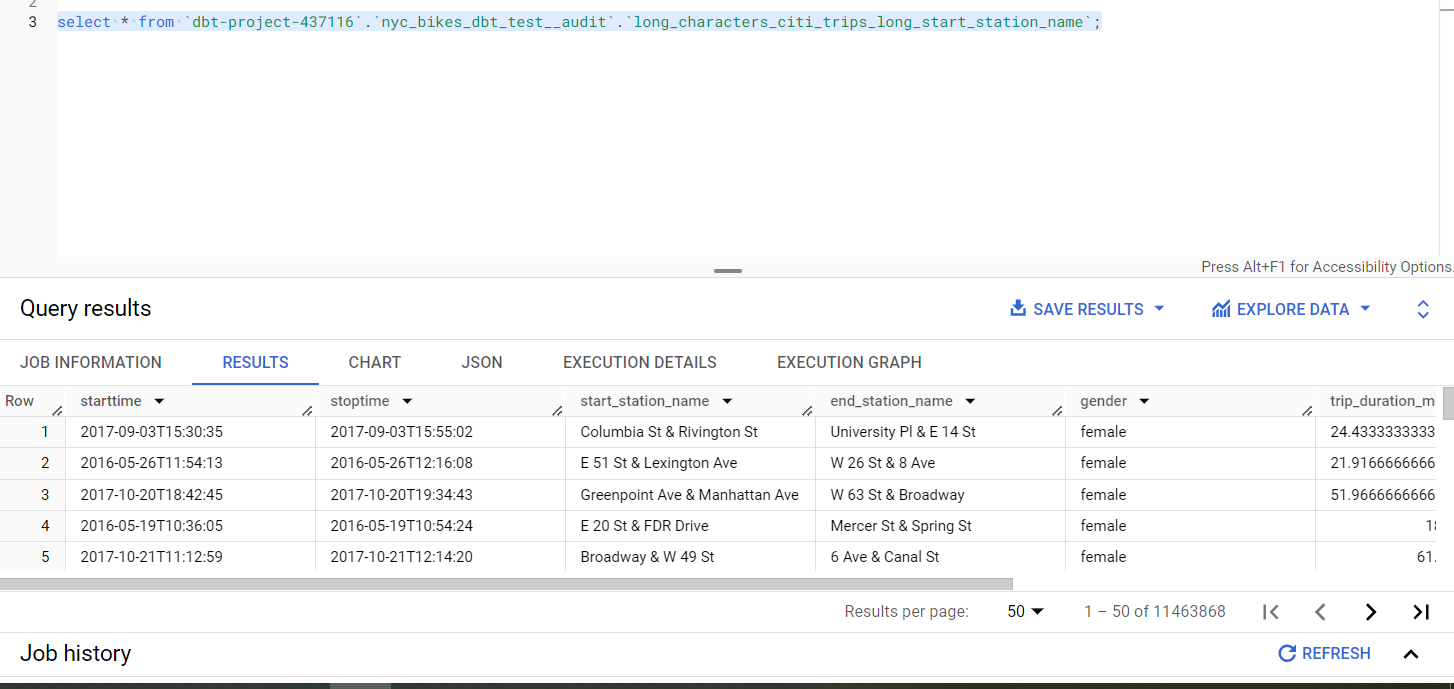
\includegraphics{./images/failing_records.png}
\caption{Failing records}
\end{figure}

That's a very convenient one-liner!

Below are other forms of generic tests shipped with dbt, for the \texttt{accepted\_values} and \texttt{relationships}. The latter took too long to run and was cancelled midway.

\begin{verbatim}
- name: end_station_name
        description: "End Station Name"
         tests:
            - relationships:
                to: ref('citi_trips_round')
                field: end_station_name

      - name: gender
        description: "Gender (unknown, male, female)"
        tests:
          - accepted_values:
              values: ['unknown', 'male', 'female']
\end{verbatim}

It's been quite an exciting journey with tests. And for sure dbt tests do grill your data!

\hypertarget{dbt-expectations-package}{%
\chapter{dbt Expectations package}\label{dbt-expectations-package}}

What is dbt-expectations? dbt-expectations is an extension package for dbt which works much akin to the Great Expectations package for Python. It was intentionally designed to provide Great Expectations like features in dbt, but now from dbt itself rather than integrating Great Expectations (GE).

Unless you've used GE, you may be wondering what this is in the first place, and its okay to feel lost. GE is much like tests in the previous chapter, it conducts quality tests on your data, thus flagging those that deviate from the set assertions.

I would put dbt-expectations and GE on the same plane and use an allegory to drive the point home: that of a car. When buying a car, there are some common checklist items, and others bespoke depending on your car model. For example, an ordinary car must have the following features (at least most of them):

\begin{itemize}
\tightlist
\item
  have four wheels
\item
  have a driver's seat
\item
  have a gear (whether manual or automatic)
\item
  have headlights
\item
  have a windshield
\end{itemize}

The above list can go on and on depending on your knowledge of cars. But your checklist can also contain some unique items, but which are a must-have depending on your car make. For example, here is a checklist of the Volvo XC60 T6:

\begin{itemize}
\tightlist
\item
  0.9l/100km fuel consumption
\item
  Allowed emissions 22g/km (the less the better)
\item
  Hybrid fuel type
\end{itemize}

So if you go to a showrooms and the beautiful or handsome sales agent takes you to the Volvo XC60, you will be perusing it as you cross your checklist. dbt-expectations and GE work in the same way.

\hypertarget{dbt-expectations-installation}{%
\section{\texorpdfstring{\texttt{dbt-expectations} installation}{dbt-expectations installation}}\label{dbt-expectations-installation}}

According to the \href{https://hub.getdbt.com/calogica/dbt_expectations/latest/}{documentation} dbt-expectations will work for dbt versions 1.7x and higher. Let's first pass this little test.

\begin{verbatim}
dbt --version
\end{verbatim}

If you get your dbt-core version is above 1.7x, then you can proceed. If not, you need to update your dbt. You can do so using \texttt{python\ -m\ pip\ install\ -\/-upgrade\ dbt-core} or if you want to be more specific, this will do: \texttt{python\ -m\ pip\ install\ -\/-upgrade\ dbt-core==0.19.0}.

Ours, at the moment of writing this book, was version \texttt{1.8.7}. Therefore we have a clean bill of health to proceed.

dbt-expectations isn't installed in the same \emph{type and enter} kind of means like we did for \texttt{dbt-core} and \texttt{dbt\ big-query}. Nevertheless, some code is written in some YAML files and from henceforth dbt recognises it.

First create a \texttt{packages.yml} file in the same level as your \texttt{dbt\_project.yml} file. You can do so by running this command:

\begin{verbatim}
touch packages.yml
\end{verbatim}

On the \texttt{packages.yml} file, insert the following:

\begin{verbatim}
packages:
  - package: calogica/dbt_expectations
    version: [">=0.10.0", "<0.11.0"]
\end{verbatim}

Apart from that, the \texttt{dbt-date} dependency must also be installed. This is because \texttt{dbt-expectations} references it. However, this will be installed in the \texttt{dbt\_project.yml} file rather than the \texttt{packages.yml} file. So inside the \texttt{dbt\_project.yml} paste the following just before the \texttt{materializations} dictionary.

\begin{verbatim}
vars:
  'dbt_date:time_zone': 'Africa/Nairobi'
\end{verbatim}

You may insert any valid timezone apart from the one specified above, but we highly suggest that you use your timezone.

Now run \texttt{dbt\ deps} to seal the deal by installing the \texttt{dbt-expectations} package.

\begin{verbatim}
dbt deps
\end{verbatim}

Here is the output showing the successful installation of the package in our environment.

\begin{verbatim}
19:31:10  Running with dbt=1.8.7
19:31:12  Updating lock file in file path: /home/sammigachuhi/dbt_book2/dbt_book/package-lock.yml
19:31:13  Installing calogica/dbt_expectations
19:31:44  Installed from version 0.10.4
19:31:44  Up to date!
19:31:44  Installing calogica/dbt_date
19:31:45  Installed from version 0.10.1
19:31:45  Up to date!
\end{verbatim}

\hypertarget{types-of-dbt-expectations-tests}{%
\section{\texorpdfstring{Types of \texttt{dbt-expectations} tests}{Types of dbt-expectations tests}}\label{types-of-dbt-expectations-tests}}

\texttt{dbt-expectations} comes with a plethora of tests' functions which can be classified into the following categories.

\begin{itemize}
\tightlist
\item
  Table shape
\item
  Missing values, unique values, and types
\item
  Sets and ranges
\item
  String matching
\item
  Aggregate functions
\item
  Multi-column
\item
  Distributional functions
\end{itemize}

We will perform one test in each category just to exemplify the potential of \texttt{dbt-expectations}.

\hypertarget{table-shape}{%
\subsection{Table shape}\label{table-shape}}

\hypertarget{expect_table_row_count_to_equal_other_table}{%
\subsubsection{\texorpdfstring{\texttt{expect\_table\_row\_count\_to\_equal\_other\_table}}{expect\_table\_row\_count\_to\_equal\_other\_table}}\label{expect_table_row_count_to_equal_other_table}}

Description: Expect the number of rows in a model match another model.

We will expect the \texttt{citi\_trips\_round} and the \texttt{citi\_trips\_minutes} tables to have the same number of rows since their respective models used the same \texttt{citi\_bike\_trips} table. Therefore, the two tables should pass this test, or will they?

Since we only want to concentrate on the models within the \texttt{my\_models} directory, just run: \texttt{dbt\ test\ -\/-select\ models/my\_models}

Here is the output.

\begin{verbatim}
-- snip --
07:57:38  2 of 8 FAIL 1 dbt_expectations_expect_table_row_count_to_equal_other_table_citi_trips_minutes_ref_citi_trips_round_  [FAIL 1 in 4.83s]
07:57:38  3 of 8 START test dbt_expectations_expect_table_row_count_to_equal_other_table_citi_trips_round_ref_citi_trips_minutes_  [RUN]
07:57:42  3 of 8 FAIL 1 dbt_expectations_expect_table_row_count_to_equal_other_table_citi_trips_round_ref_citi_trips_minutes_  [FAIL 1 in 4.53s]
-- snip --
\end{verbatim}

This leaves one puzzled, why?

A close look at the model for \texttt{citi\_trips\_round} reveals the answer. This model was designed to only work on non-null rows, unlike the \texttt{citi\_trips\_minutes} which worked on all rows, null or not. Therefore the \texttt{citi\_trips\_round} had less rows and thus the generated the error. In case your tests results seem incongruent, it is always good to recheck the models to refresh your memory, as we did here.

In fact, dbt did a good job of generating an SQL to show us the error:

\begin{verbatim}
07:58:03  Failure in test dbt_expectations_expect_table_row_count_to_equal_other_table_citi_trips_minutes_ref_citi_trips_round_ (models/my_models/my_models.yml)
07:58:03    Got 1 result, configured to fail if != 0
07:58:03  
07:58:03    compiled code at target/compiled/dbt_book/models/my_models/my_models.yml/dbt_expectations_expect_table__c00100dada30a31f15f90b9c1ba0b295.sql
\end{verbatim}

If you click on the destination of the SQL statement and copy the contents to the SQL query tab of BigQuery, you will see the difference in row count for the two tables.

\begin{figure}
\centering
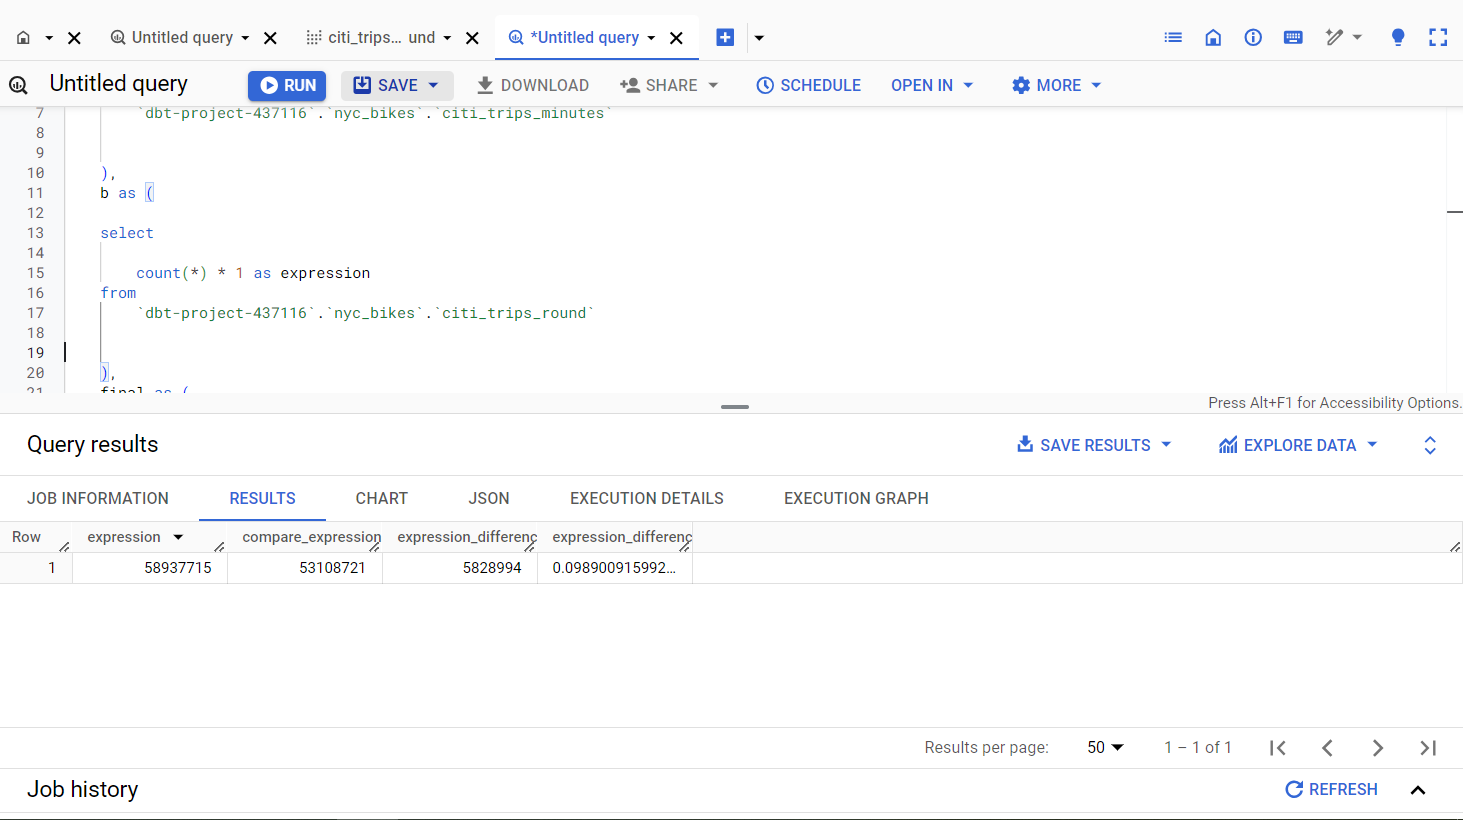
\includegraphics{./images/row_count_difference.png}
\caption{Row count difference}
\end{figure}

\hypertarget{missing-values-unique-values-and-types}{%
\subsection{Missing values, unique values, and types}\label{missing-values-unique-values-and-types}}

\hypertarget{expect_column_values_to_not_be_null}{%
\subsubsection{\texorpdfstring{\texttt{expect\_column\_values\_to\_not\_be\_null}}{expect\_column\_values\_to\_not\_be\_null}}\label{expect_column_values_to_not_be_null}}

Description: Expect column values to not be null.

This is a \emph{no-brainer} kind of test. Can you guess which columns in any of our tables in the \texttt{nyc\_bikes} dataset should never be null? Here is a clue, station\_id and station names, unless the biker teleports to or from somewhere!

So on the \texttt{my\_models} YAML file, insert the below test on the \texttt{start\_station\_id}, \texttt{start\_station\_name}, \texttt{end\_station\_id} and \texttt{end\_station\_name} fields.

\begin{verbatim}
tests:
  - dbt_expectations.expect_column_values_to_not_be_null
\end{verbatim}

You will get some interesting results. some of the tests fail for the \texttt{citi\_trips\_minutes} model because of the many null rows in the table. However, none of this particular test fail for the \texttt{citi\_trips\_round} table; it has zero null rows.

A caveat when using the \texttt{dbt\_expectations.expect\_column\_values\_to\_not\_be\_null}, only add a colon \texttt{:} when specifying more optional parameters such as \texttt{row\_condition:\ "id\ is\ not\ null"\ \#\ (Optional)}. Otherwise, leave it out.

\hypertarget{sets-and-ranges}{%
\subsection{Sets and Ranges}\label{sets-and-ranges}}

\hypertarget{expect_column_values_to_be_in_set}{%
\subsubsection{\texorpdfstring{\texttt{expect\_column\_values\_to\_be\_in\_set}}{expect\_column\_values\_to\_be\_in\_set}}\label{expect_column_values_to_be_in_set}}

Description: Expect each column value to be in a given set.

This test works best for where you are sure that a certain column will only accept certain values. A good example is the \texttt{gender} column. There can only be three results: male, female and other. Here we insert the test in our \texttt{citi\_trips\_minutes} and \texttt{citi\_trips\_round} models.

\begin{verbatim}
- name: gender
  description: "Gender (unknown, male, female)"
  tests:
    - dbt_expectations.expect_column_values_to_be_in_set:
        value_set: ['unknown','male','female']
\end{verbatim}

If you run the above test for both the \texttt{citi\_trips\_minutes} and \texttt{citi\_trips\_round} models, the test will fail for the former. Why, because of the pesky null rows. However, to take the null rows into consideration and take them as accepted values in the \texttt{citi\_trips\_minutes} model only, we simply add an empty quotation marks, like so (\texttt{\textquotesingle{}\textquotesingle{}}). Here is our modified test: \texttt{value\_set:\ {[}\textquotesingle{}\textquotesingle{},\ \textquotesingle{}unknown\textquotesingle{},\textquotesingle{}male\textquotesingle{},\textquotesingle{}female\textquotesingle{}{]}}. The test will then pass for our \texttt{citi\_trips\_minutes} table.

\hypertarget{string-matching}{%
\subsection{String matching}\label{string-matching}}

\hypertarget{expect_column_value_lengths_to_be_between}{%
\subsubsection{\texorpdfstring{\texttt{expect\_column\_value\_lengths\_to\_be\_between}}{expect\_column\_value\_lengths\_to\_be\_between}}\label{expect_column_value_lengths_to_be_between}}

Description: Expect column entries to be strings with length between a min\_value value and a max\_value value (inclusive).

Because our \texttt{citi\_trips\_minutes} table has several null rows, we will put the minimum expected value to be 0. Since we also want to catch those station names with overly long names, we will put the max value as 70. So for both the \texttt{start\_station\_name} and the \texttt{end\_station\_name}, we inserted the following test:

\begin{verbatim}
tests:
  - dbt_expectations.expect_column_values_to_not_be_null
  - dbt_expectations.expect_column_value_lengths_to_be_between:
      min_value: 1 # (Optional)
      max_value: 70 # (Optional)
\end{verbatim}

We are glad to know both models passed this simple test.

\hypertarget{aggregate}{%
\subsection{Aggregate}\label{aggregate}}

\hypertarget{expect_column_max_to_be_between}{%
\subsubsection{\texorpdfstring{\texttt{expect\_column\_max\_to\_be\_between}}{expect\_column\_max\_to\_be\_between}}\label{expect_column_max_to_be_between}}

Description: Expect the column max to be between a min and max value

You may wonder what the purpose of this test is. But don't dismiss it yet, it can come quite in handy when searching for outlier values. We will demonstrate it in catching overly long bike trips. However, this test needs some background knowledge of your data.

Applying the below queries on BigQuery will help.

\begin{verbatim}
SELECT AVG(trip_duration_min) FROM dbt-project-437116.nyc_bikes.citi_trips_minutes; -- 16

SELECT MAX(trip_duration_min) FROM dbt-project-437116.nyc_bikes.citi_trips_minutes; -- 325167.48

SELECT * FROM dbt-project-437116.nyc_bikes.citi_trips_minutes
WHERE trip_duration_min > 200000;
\end{verbatim}

Now lets place the limits of our maximum trip duration values to be between the average of 16 and some intermediate value such as 100, 000 minutes (1, 666 hours)!

\begin{verbatim}
tests:
  - dbt_expectations.expect_column_max_to_be_between:
      min_value: 16 # (Optional)
      max_value: 100000 # (Optional)
\end{verbatim}

That will flag off some errors, but if you change the \texttt{max\_value} parameter to \texttt{360000}, the tests will pass. However, in the \texttt{trip\_min\_round} field of the \texttt{citi\_trips\_round} model, we set the \texttt{max\_value} as 100000 to demonstrate an error of this test.

\hypertarget{multi-column}{%
\subsection{Multi-column}\label{multi-column}}

\hypertarget{expect_column_pair_values_a_to_be_greater_than_b}{%
\subsubsection{\texorpdfstring{\texttt{expect\_column\_pair\_values\_A\_to\_be\_greater\_than\_B}}{expect\_column\_pair\_values\_A\_to\_be\_greater\_than\_B}}\label{expect_column_pair_values_a_to_be_greater_than_b}}

Description: Expect values in column A to be greater than column B.

This kind of test comes in handy when you want to ensure that one of your columnar values is greater than, or less than that of a different column. A good example is a comparison of trip duration in seconds in the \texttt{tripduration} column versus the trip duration in minutes from \texttt{trip\_min\_round} column in our \texttt{citi\_trips\_round} table. Definitely time in seconds will always have a greater value in terms of length than the more concise minutes values!

In our \texttt{citi\_trips\_round} model, insert the test as follows:

\begin{verbatim}
- name: citi_trips_round
    description: '{{ doc("citi_trips_round") }}'
    tests:
      - dbt_expectations.expect_table_row_count_to_equal_other_table:
          compare_model: ref("citi_trips_minutes")
      - dbt_expectations.expect_column_pair_values_A_to_be_greater_than_B:
          column_A: tripduration
          column_B: trip_min_round
\end{verbatim}

It surely does pass the test.

\begin{verbatim}
-- snip --
09:40:46  5 of 26 PASS dbt_expectations_expect_column_pair_values_A_to_be_greater_than_B_citi_trips_round_tripduration__trip_min_round  [PASS in 2.20s]
\end{verbatim}

\hypertarget{distributional-functions}{%
\subsection{Distributional functions}\label{distributional-functions}}

This is another category of shipped-in tests of \texttt{dbt-expectations}. However, they require some statistical homework to be conducted on your data prior to applying the tests. The tests under this category include: \texttt{expect\_column\_values\_to\_be\_within\_n\_moving\_stdevs}, \texttt{expect\_column\_values\_to\_be\_within\_n\_stdevs} and \texttt{expect\_row\_values\_to\_have\_data\_for\_every\_n\_datepart}.

\hypertarget{seeds}{%
\chapter{Seeds}\label{seeds}}

Seeds are Comma Separated Values (csv) files stored inside your \texttt{seeds} directory which can be loaded into your data warehouse using the \texttt{dbt\ seed} command.

Seeds can also be referenced by your SQL models using the \texttt{ref()} function. Seeds in dbt are version controlled. That is, you can revert them to a previous state.

Seeds are best used for data that changes infrequently. A good example is country codes, email accounts and station names. However, seeds should not be used to store sensitive information such as passwords.

To demonstrate about seeds in dbt, we will try to upload a \href{https://www.civicdata.com/dataset/nyc-bike-share-trip-data/resource/3e7acf34-19ba-4bf4-8dd2-cf349623dc6b}{New York City (NYC) bike history data} for 2014.

Extract the zip folder and copy the \texttt{3e7acf34-19ba-4bf4-8dd2-cf349623dc6b.csv} inside the \texttt{dbt\_book/seeds} directory. To reduce the verbosity of its name, rename it to \texttt{2014-tripdata.csv}.

\hypertarget{uploading-a-seed-into-your-data-warehouse}{%
\section{Uploading a seed into your data warehouse}\label{uploading-a-seed-into-your-data-warehouse}}

Believe you me we had a better csv table to upload, one much more related to the NYC bikes dataset. However, because it was \textasciitilde320MB and we want to be economical in upload times and bandwith, we settled for this historical data. Nevertheless, keeping on with this chapter, to upload a seed into a data warehouse, we use this command:

\begin{verbatim}
dbt seed
\end{verbatim}

After that, it's a test of patience. Depending on your upload speeds, it shouldn't take long to upload a 36MB file to BigQuery.

\begin{verbatim}
-- snip --
16:31:51  Concurrency: 1 threads (target='dev')
16:31:51  
16:31:51  1 of 1 START seed file nyc_bikes.2014-tripdata ................................. [RUN]
16:33:17  1 of 1 OK loaded seed file nyc_bikes.2014-tripdata ............................. [INSERT 224736 in 85.39s]
16:33:17  
16:33:17  Finished running 1 seed in 0 hours 1 minutes and 28.54 seconds (88.54s).
16:33:17  
16:33:17  Completed successfully
16:33:17  
16:33:17  Done. PASS=1 WARN=0 ERROR=0 SKIP=0 TOTAL=1
\end{verbatim}

If you go to BigQuery and refresh the contents of your \texttt{nyc\_bikes} dataset, you should see the \texttt{2014-tripdata} table present.

\begin{figure}
\centering
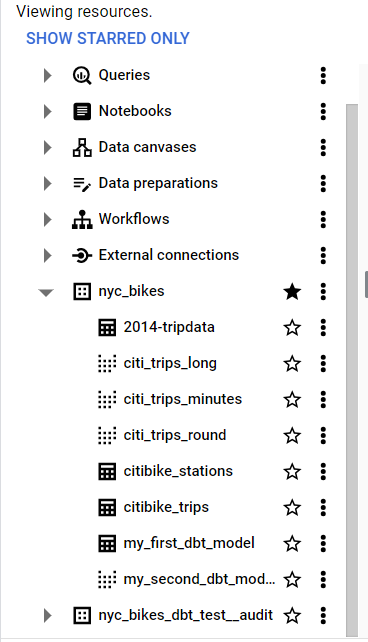
\includegraphics{./images/2014-tripdata.png}
\caption{Seeds}
\end{figure}

\hypertarget{referencing-seeds-in-models}{%
\section{Referencing seeds in models}\label{referencing-seeds-in-models}}

Just like you would reference a model in another model, we can also reference seeds in another model. All your need to reference a seed is to place the name of the csv file, excluding the \texttt{.csv} extension inside the \texttt{ref()} function.

For example, we want to create a view that contains those start station names from our 2014 table that are existent in the \texttt{citi\_trips\_long} model.

Within the \texttt{models/my\_models} directory, create the \texttt{citi\_stations\_2014.sql} model with the following query:

\begin{verbatim}
{{ config(materialized='view') }}

WITH citi_stations_2014 AS (
    SELECT * FROM {{ref ('2014-tripdata') }}
    WHERE `start station name` IN (
        SELECT start_station_name FROM {{ ref('citi_trips_long') }}
    )
)

SELECT * FROM citi_stations_2014
\end{verbatim}

Thereafter, run the model using \texttt{dbt\ run\ -\/-select\ citi\_stations\_2014}

That will create a view that contains only those stations within the \texttt{2014-tripdata.csv} also within the \texttt{citi\_trips\_long} model. Much to our surprise, all the stations within our 2014 table are also found in the \texttt{citi\_trips\_long} model!

Here are the SQL queries we used to perform a count of each of the two tables in BigQuery.

\begin{verbatim}
SELECT COUNT(*) FROM `dbt-project-437116`.`nyc_bikes`.`2014-tripdata`;

SELECT COUNT(*) FROM dbt-project-437116.nyc_bikes.citi_stations_2014;
\end{verbatim}

Both returned a value of \texttt{224736}.

Here is the view of the \texttt{citi\_stations\_2014} model in BigQuery.

\begin{figure}
\centering
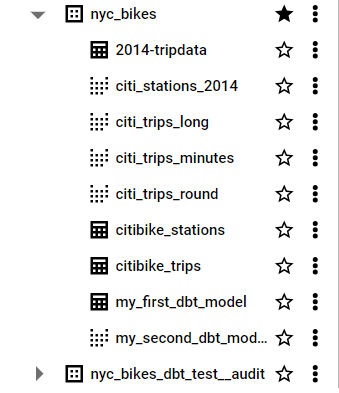
\includegraphics{./images/seed_view.png}
\caption{View from seed}
\end{figure}

\hypertarget{seed-configurations-at-project-level}{%
\section{Seed Configurations at project level}\label{seed-configurations-at-project-level}}

Though it may sound like there is a lot to do here, there actually isn't. Suffice to only say that seeds are configurable as much as our normal models are. There are two ways to \href{https://docs.getdbt.com/reference/seed-configs}{configure seeds} in dbt: either in the \texttt{dbt\_project} YAML file or at the individual seed's YAML properties.

For the purposes of this exercise, at the project level we will set a dictionary that looks as follows:

\begin{verbatim}
seeds:
  dbt_book:
    2014-tripdata:
      schema: nyc2014_data
\end{verbatim}

For any \href{https://docs.getdbt.com/reference/resource-configs/schema}{custom schema} that we set, the result will be in the following format: \texttt{\{\{\ target.schema\ \}\}\_\{\{\ schema\ \}\}.} That means the expected schema for our seed will be \texttt{nyc\_bikes\_nyc2014\_data} --quite a mouthful of a name.

Thereafter run \texttt{dbt\ seed}.

\begin{verbatim}
-- snip --
19:24:43  Concurrency: 1 threads (target='dev')
19:24:43  
19:24:43  1 of 1 START seed file nyc_bikes_nyc2014_data.2014-tripdata .................... [RUN]
19:26:18  1 of 1 OK loaded seed file nyc_bikes_nyc2014_data.2014-tripdata ................ [INSERT 224736 in 95.10s]
19:26:18  
19:26:18  Finished running 1 seed in 0 hours 1 minutes and 46.50 seconds (106.50s).
19:26:18  
19:26:18  Completed successfully
19:26:18  
19:26:18  Done. PASS=1 WARN=0 ERROR=0 SKIP=0 TOTAL=1
\end{verbatim}

Think of a schema as a folder or container for storing your data (read tables). Therefore, if you were in a company, there would be a schema (read it as folder or container) for sales, customers, products and clients. Inside the schema, (read folder or container) for sales, there would be tables for \texttt{january\_sales}, \texttt{february\_sales} and so on.

Just a \emph{nota bene}, don't use hyphens \texttt{(-)} for your schema names, otherwise it will result in an error.

Here is our seed data appearing under the \texttt{nyc\_bikes\_nyc2014\_data} dataset.

\begin{figure}
\centering
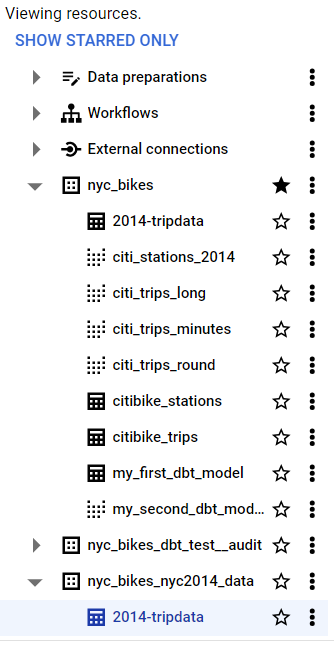
\includegraphics{./images/seeds_schema.png}
\caption{Schema for seeds}
\end{figure}

\hypertarget{seed-properties-and-configurations-at-properties-level}{%
\section{Seed properties and configurations at properties level}\label{seed-properties-and-configurations-at-properties-level}}

Seeds can also be configured at the properties level. In fact, the configurations at the properties level will override those set at the project level, that is at the \texttt{dbt\_project} file.

To demonstrate setting seed configurations at the properties level, create \texttt{nyc\_bikes2014} YAML file. Copy paste the following contents into the file.

\begin{verbatim}
version: 2

seeds:
  - name: 2014-tripdata
    description: "Seed for NYC 2014 bike data"
    docs:
      show: true 
      node_color: purple # Use name (such as node_color: purple) or hex code with quotes (such as node_color: "#cd7f32")
    config:
      schema: nyc_bikes2014
\end{verbatim}

Not much different from the model properties' files we create, isn't it? In this case, the \texttt{name} of the model is not a SQL file but the csv we pushed to the data warehouse. The \texttt{docs} key is not so much important as the \texttt{config} key which we use to set the schema of our seed in the data warehouse.

What's good for the goose is good for the gander. Much akin to the model properties files were we can insert tests and documentation, the same goes for seed properties' files. In the contents of the below properties file of \texttt{nyc\_bikes2014.yml} we have inserted documentation at both the table and column levels. We have also inserted tests at both levels as well.

\begin{verbatim}
version: 2

seeds:
  - name: 2014-tripdata
    description: '{{ doc("seed_2014_tripdata") }}'
    docs:
      show: true 
      node_color: purple # Use name (such as node_color: purple) or hex code with quotes (such as node_color: "#cd7f32")
    config:
      schema: nyc_bikes2014
    tests:
      - dbt_expectations.expect_table_column_count_to_be_between:
          min_value: 1 # (Optional)
    columns:
      - name: _id
        description: 'Unique identifier'
        tests:
          - dbt_expectations.expect_column_values_to_be_unique

      - name: tripduration
        description: '{{ doc("tripduration") }}'
\end{verbatim}

If you have additional seeds, simply add them to the properties files much like what we have in the \texttt{my\_models.yml} which consists of the three models \texttt{citi\_trips\_minutes}, \texttt{citi\_trips\_round} and \texttt{citi\_trips\_long}.

\hypertarget{performing-tests-on-seeds}{%
\section{Performing tests on seeds}\label{performing-tests-on-seeds}}

Tests on seeds are performed in much the same way as other models. The only trick is to insert the name of the csv file. For example, to run a test of our \texttt{2014-tripdata.csv} which is our seed model, we execute \texttt{dbt\ test\ -\/-select\ 2014-tripdata}.

\begin{verbatim}
-- snip --
18:19:53  Concurrency: 1 threads (target='dev')
18:19:53  
18:19:53  1 of 2 START test dbt_expectations_expect_column_values_to_be_unique_2014-tripdata__id  [RUN]
18:19:57  1 of 2 PASS dbt_expectations_expect_column_values_to_be_unique_2014-tripdata__id  [PASS in 4.67s]
18:19:57  2 of 2 START test dbt_expectations_expect_table_column_count_to_be_between_2014-tripdata_1  [RUN]
18:20:02  2 of 2 PASS dbt_expectations_expect_table_column_count_to_be_between_2014-tripdata_1  [PASS in 4.58s]
18:20:02  
18:20:02  Finished running 2 data tests in 0 hours 0 minutes and 12.62 seconds (12.62s).
18:20:02  
18:20:02  Completed successfully
-- snip --
\end{verbatim}

As you can see, the two tests of \texttt{dbt\_expectations.expect\_table\_column\_count\_to\_be\_between} and \texttt{dbt\_expectations.expect\_column\_values\_to\_be\_unique} passed.

\hypertarget{viewing-documentation-for-dbt-seeds}{%
\section{Viewing documentation for dbt seeds}\label{viewing-documentation-for-dbt-seeds}}

Even much less different than running tests is the generation of documentation regarding your dbt seeds. The process is exactly the same. First, run \texttt{dbt\ docs\ generate}. Assuming that the manifest files have successfully been created in the catalog, run \texttt{dbt\ docs\ serve}. If no errors appear at this final stage, open the port link that appears, such as \texttt{localhost:8080/}, on the terminal in your preferred browser.

You should see the documentation you created for your seed. The lineage graph should also work well for the seeds too.

\begin{figure}
\centering
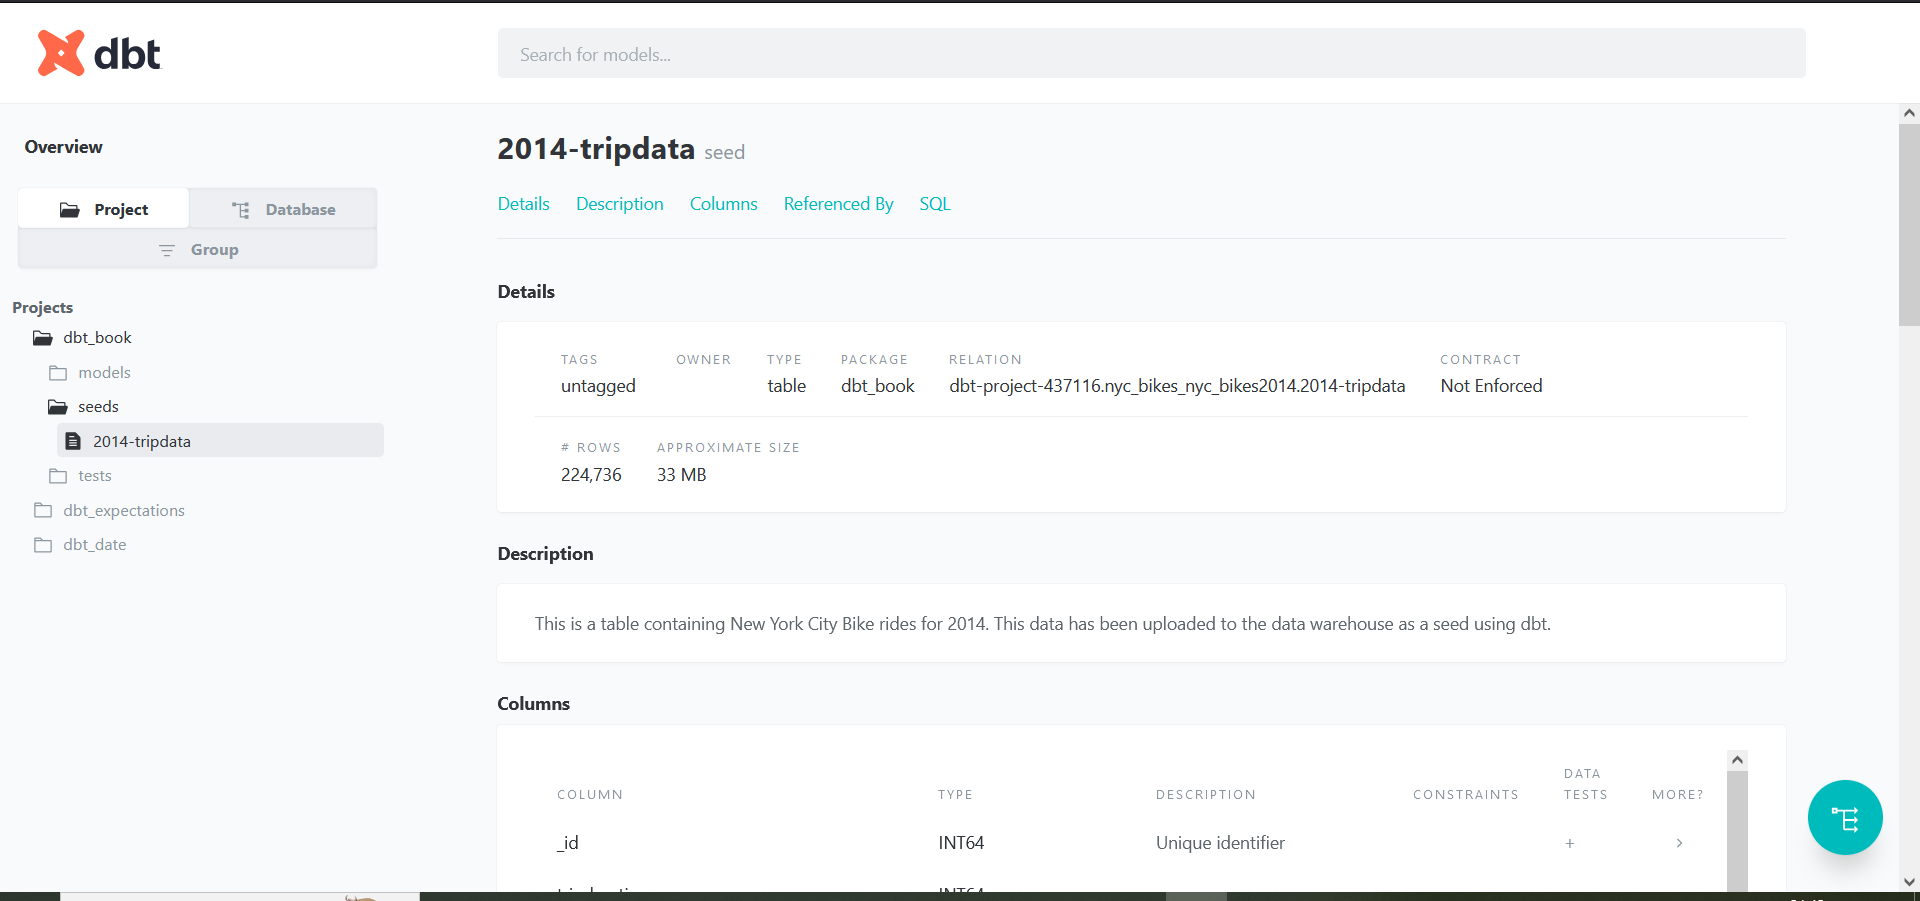
\includegraphics{./images/seed_documentation.png}
\caption{Documentation on seeds}
\end{figure}

Every seed at some point is left to grow on its own. We suppose this chapter has provided the necessary nutrition to see you bud to life working with dbt seeds.

\hypertarget{sources-1}{%
\chapter{Sources}\label{sources-1}}

In the all-time favourite book \emph{The voyages and adventures of Captain Hatteras}, every morning, the second-in-command, a well versed captain of the high seas, Richard Shandon by name, would receive a letter from an anonymous sender directing him on which direction to steer the ship. In dbt, sources are what make your data in the data warehouse be referenced in dbt operations such as running models, tests and checking the `freshness' of your data.

Just like in the above anecdote where, if any person in the crew would ask Sir Richard Shandon for justification of any task they were commanded to do, Richard would always refer to the authoritative letter from an anonymous source. Likewise, when working with sources, dbt will perform operations by referencing the sources using the \texttt{source} function (\texttt{\{\{\ source("schema",\ "table")\ \}\}}).

Sources in dbt are defined inside YAML files, and they are referenced inside SQL files, just like regular models again!

\hypertarget{defining-a-source}{%
\section{Defining a source}\label{defining-a-source}}

To demonstrate defining sources, we will work with two tables already in our data warehouse. These are the \texttt{2014-tripdata} and \texttt{citi\_trips\_round} tables under \texttt{nyc\_bikes\_nyc\_bikes2014} (\texttt{nyc\_bikes\_nyc\_bikes2014/2014-tripdata}) and \texttt{nyc\_bikes} tree structures in BigQuery respectively.

Create a new sibling directory called \texttt{sources} next to the \texttt{docs}, \texttt{example}, and \texttt{my\_models} folders. Inside it, create a new YAML file called \texttt{sources\_bikes.yml}. The path to this file should be \texttt{models/sources/sources\_bikes.yml}.

Copy paste these contents into the newly created YAML file.

\begin{verbatim}
version: 2

sources:
  - name: nyc_bikes_nyc_bikes2014
    schema: nyc_bikes_nyc_bikes2014
    tables:
      - name: 2014-tripdata

  - name: nyc_bikes
    schema: nyc_bikes 
    tables:
      - name: citi_trips_round
\end{verbatim}

The above should be all too familiar since we've worked with several YAML files so far. Nevertheless, the \texttt{name} and \texttt{schema} values refer to the schema names in your data warehouse. For the \texttt{tables} dictionary, we refer to the names of those tables under a particular schema. For example, the \texttt{citi\_trips\_round} is definitely under the \texttt{nyc\_bikes} schema.

\hypertarget{referencing-sources}{%
\section{Referencing sources}\label{referencing-sources}}

Sources in our data warehouse are referenced using the \texttt{source()} function. Remember when referencing other models within models we used the \texttt{ref()} function? When working with sources, the \texttt{ref()} is now \texttt{source()}.

Below is a demonstration of referencing a source to only select male bike riders. Notice the arrangement of the schema and table names within quotation marks (\texttt{\textquotesingle{}\textquotesingle{}}) and separated by a comma. This is how we reference other data acting as the \emph{source} in our \texttt{nyc\_bikes\_male.sql}.

\begin{verbatim}
SELECT * FROM 
{{ source('nyc_bikes', 'citi_trips_round') }}
WHERE gender = "male"
\end{verbatim}

The same also works for data uploaded as a seed in our data warehouse as seen in the \texttt{nyc\_male\_2014.sql}.

\begin{verbatim}
SELECT * FROM 
{{ source('nyc_bikes_nyc_bikes2014', '2014-tripdata') }}
WHERE gender = 1
\end{verbatim}

We run these two specific models using \texttt{dbt\ run\ -\/-select\ sources} and we get this output:

\begin{verbatim}
19:29:52  Concurrency: 1 threads (target='dev')
19:29:52  
19:29:52  1 of 2 START sql view model nyc_bikes.nyc_bikes_male ........................... [RUN]
19:29:56  1 of 2 OK created sql view model nyc_bikes.nyc_bikes_male ...................... [CREATE VIEW (0 processed) in 3.74s]
19:29:56  2 of 2 START sql view model nyc_bikes.nyc_male_2014 ............................ [RUN]
19:29:59  2 of 2 OK created sql view model nyc_bikes.nyc_male_2014 ....................... [CREATE VIEW (0 processed) in 3.29s]
19:29:59  
19:29:59  Finished running 2 view models in 0 hours 0 minutes and 12.75 seconds (12.75s).
19:30:00  
19:30:00  Completed successfully
19:30:00  
19:30:00  Done. PASS=2 WARN=0 ERROR=0 SKIP=0 TOTAL=2
\end{verbatim}

If you check under the \texttt{nyc\_bikes} schema in your BigQuery, you will notice two new views have been created: \texttt{nyc\_bikes\_male} and \texttt{nyc\_male\_2014}.

\begin{figure}
\centering
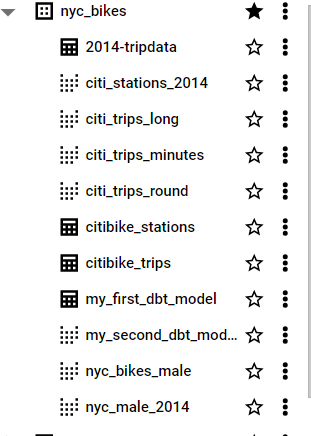
\includegraphics{./images/sources.png}
\caption{Sources}
\end{figure}

One would have expected the \texttt{nyc\_male\_2014} view to be under the \texttt{nyc\_bikes\_nyc\_bikes2014} schema because that's the seed dataset. Our assumption is that we set the \texttt{nyc\_bikes} as the dataset to work with when setting up dbt, and thus it's very hard to deviate from this. But we stand to be corrected. One more thing, the dbt source can also work inside a \texttt{WITH} SQL statement like so in the \texttt{nyc\_female\_2014} model.

\begin{verbatim}
WITH nyc_female_2014 AS (
    SELECT * FROM 
        {{ source('nyc_bikes_nyc_bikes2014', '2014-tripdata') }}
    WHERE gender = 2
)

SELECT * FROM nyc_female_2014
\end{verbatim}

\hypertarget{defining-properties-in-a-sources-file}{%
\section{\texorpdfstring{Defining properties in a \texttt{sources} file}{Defining properties in a sources file}}\label{defining-properties-in-a-sources-file}}

Just like you would craft the properties for a given models' YAML file, the same can likewise be done for the sources YAML file. You can define descriptions and tests for your fields in a \texttt{sources} file. Again, what's good for the goose is good for the gander. Below is our enriched \texttt{sources} YAML file.

\begin{verbatim}
version: 2

sources:
  - name: nyc_bikes_nyc_bikes2014
    schema: nyc_bikes_nyc_bikes2014
    tables:
      - name: 2014-tripdata
        description: '{{ doc("tripduration") }}'
        columns:
          - name: _id 
            description: 'Unique id'
            tests:
              - dbt_expectations.expect_column_values_to_not_be_null

          - name: tripduration 
            description: '{{ doc("tripduration") }}'

          - name: starttime 
            description: ''

          - name: stoptime 
            description: ''

          - name: start station id 
            description: ''

          - name: start station name
            description: ''

          - name: start station latitude
            description: ''

          - name: start station longitude
            description: ''

          - name: end station id
            description: ''

          - name: end station name
            description: ''

          - name: end station latitude
            description: ''

          - name: end station longitude
            description: ''

          - name: bikeid
            description: ''

          - name: usertype
            description: ''

          - name: birth year
            description: ''

          - name: gender
            description: ''

  - name: nyc_bikes
    schema: nyc_bikes 
    tables:
      - name: citi_trips_round
\end{verbatim}

Let's start by running the sole test at the trusty \texttt{tripduration} key via our single-line slingshot code: \texttt{dbt\ test\ -\/-select\ sources}.

Everything ran fine meaning there were no null values in this field.

\begin{verbatim}
19:32:18  Concurrency: 1 threads (target='dev')
19:32:18  
19:32:18  1 of 1 START test dbt_expectations_source_expect_column_values_to_not_be_null_nyc_bikes_nyc_bikes2014_2014-tripdata__id  [RUN]
19:32:21  1 of 1 PASS dbt_expectations_source_expect_column_values_to_not_be_null_nyc_bikes_nyc_bikes2014_2014-tripdata__id  [PASS in 3.24s]
\end{verbatim}

To see if our descriptions will be updated in the dbt documentation, simply run \texttt{dbt\ docs\ generate} followed by \texttt{dbt\ docs\ serve} to start the local server.

\begin{figure}
\centering
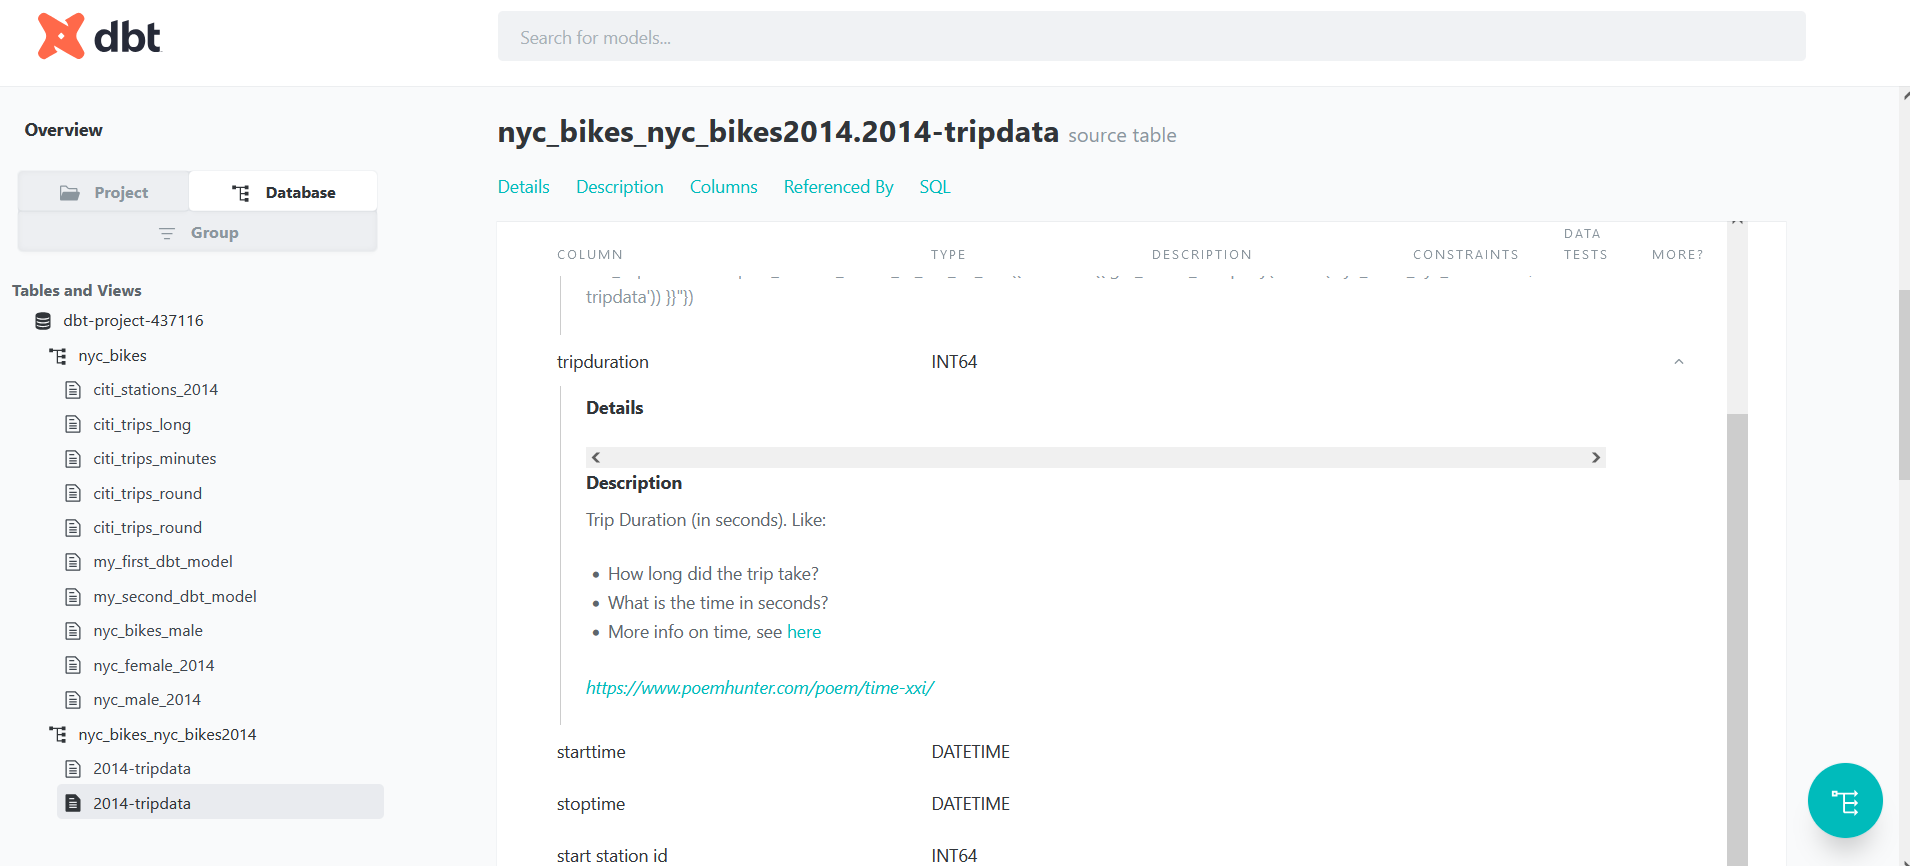
\includegraphics{./images/sources_definitions.png}
\caption{Sources descriptions}
\end{figure}

You should see your dbt documentation updated with the descriptions for \texttt{nyc\_bikes\_nyc\_bikes2014} table.

Below is our \texttt{sources} YAML file in full with additional descriptions and tests.

\begin{verbatim}
version: 2

sources:
  - name: nyc_bikes_nyc_bikes2014
    schema: nyc_bikes_nyc_bikes2014
    tables:
      - name: 2014-tripdata
        description: '{{ doc("seed_2014_tripdata") }}'
        columns:
          - name: _id 
            description: 'Unique id'
            tests:
              - dbt_expectations.expect_column_values_to_not_be_null

          - name: tripduration 
            description: '{{ doc("tripduration") }}'

          - name: starttime 
            description: ''

          - name: stoptime 
            description: ''

          - name: start station id 
            description: ''

          - name: start station name
            description: ''

          - name: start station latitude
            description: ''

          - name: start station longitude
            description: ''

          - name: end station id
            description: ''

          - name: end station name
            description: ''

          - name: end station latitude
            description: ''

          - name: end station longitude
            description: ''

          - name: bikeid
            description: ''

          - name: usertype
            description: ''

          - name: birth year
            description: ''

          - name: gender
            description: ''

  - name: nyc_bikes
    schema: nyc_bikes 
    tables:
      - name: citi_trips_round
        description: '{{ doc("citi_trips_round") }}'
        tests:
          - dbt_expectations.expect_table_row_count_to_equal_other_table:
              compare_model: ref("citi_trips_minutes")
          - dbt_expectations.expect_column_pair_values_A_to_be_greater_than_B:
              column_A: tripduration
              column_B: trip_min_round
        columns:
          - name: tripduration
            description: '{{ doc("tripduration") }}'

          - name: starttime
            description: '{{ doc("starttime") }}'
          
          - name: stoptime
            description: '{{ doc("stoptime") }}'

          - name: start_station_id
            description: "Start Station ID"
            tests:
              - dbt_expectations.expect_column_values_to_not_be_null
          
          - name: start_station_name
            description: "Start Station Name"
            tests:
              - dbt_expectations.expect_column_values_to_not_be_null
              - dbt_expectations.expect_column_value_lengths_to_be_between:
                  min_value: 1 # (Optional)
                  max_value: 70 # (Optional)

          - name: start_station_latitude
            description: "Start Station Latitude"
          
          - name: start_station_longitude
            description: "Start Station Longitude"

          - name: end_station_id
            description: "End Station ID"
            tests:
              - dbt_expectations.expect_column_values_to_not_be_null

          - name: end_station_name
            description: "End Station Name"
            tests:
              - dbt_expectations.expect_column_values_to_not_be_null
              - dbt_expectations.expect_column_value_lengths_to_be_between:
                  min_value: 1 # (Optional)
                  max_value: 70 # (Optional)

          - name: end_station_latitude
            description: "End Station Latitude"

          - name: end_station_longitude
            description: "End Station Longitude"
          
          - name: bike_id
            description: "Bike ID"
          
          - name: usertype
            description: "User Type (Customer = 24-hour pass or 7-day pass user, Subscriber = Annual Member)"

          - name: birth_year
            description: "Year of Birth"

          - name: gender
            description: "Gender (unknown, male, female)"
            tests:
              - dbt_expectations.expect_column_values_to_be_in_set:
                  value_set: ['unknown','male','female']

          - name: customer_plan
            description: "The name of the plan that determines the rate charged for the trip"

          - name: trip_duration_min
            description: '{{ doc("trip_duration_min") }}'
            tests:
              - dbt_expectations.expect_column_max_to_be_between:
                  min_value: 16 # (Optional)
                  max_value: 326000 # (Optional)

          - name: trip_min_round
            description: '{{ doc("trip_min_round") }}'
            tests:
              - dbt_expectations.expect_column_max_to_be_between:
                  min_value: 16 # (Optional)
                  max_value: 100000 # (Optional)
\end{verbatim}

\hypertarget{snapshots}{%
\chapter{Snapshots}\label{snapshots}}

Picture this, there is this lady you have been eyeing, after turning and tossing for several nights, you decide to visit her place because she is currently not anywhere interested in being taken out. When you visit her at the rendezvous, you decide to ask her to take a `selfie' of you and her (big mistake). You think she will send the selfie to you, she never does. Well, that's a true story of yours truly and even though no hard feelings over the incident, snapshots in dbt work in much the same way.

A snapshot in dbt is a recorded change of a mutable table. Think of a snapshot as a way to track changes in your data. For example, you could be a having a crazy table that logs your relationship status with your girlfriend or boyfriend over time. The first row could be as follows:

\begin{verbatim}
|----------|--------------|---------------|
| id       |  Status      | updated-at    |
| 11       |  Spark       | 21/09/2024    |
|----------|--------------|---------------|
\end{verbatim}

Now, let's say you realise something about your girlfriend and boyfriend that puts a freeze on the relationship. So in your relationship table it would have the following update.

\begin{verbatim}
|----------|--------------|---------------|
| id       |  Status      | updated-at    |
| 11       |  Shaky       | 22/10/2024    |
|----------|--------------|---------------|
\end{verbatim}

Our above update will have overwritten the previous record of `Spark' when the relationship was at cloud nine. dbt offers a way to preserve these past records so that they can be used for further analysis, or for posterity purposes. For example, keeping a record of the change can be used to analyse how long the relationship lasted from its hey days to when the waves started beating the ship. This kind of analysis can be used for more serious matters, such as when analyzing the time it takes from sending to receiving an order. dbt will help you record these changes and log the time when the change took place. For example, our dbt snapshot for our relationship would be:

\textbar----------\textbar--------------\textbar---------------\textbar----------------\textbar--------------\textbar{}
\textbar{} id \textbar{} Status \textbar{} updated-at \textbar{} dbt\_valid\_from \textbar{} dbt\_valid\_to \textbar{}
\textbar{} 11 \textbar{} Spark \textbar{} 21/09/2024 \textbar{} 21/09/2024 \textbar{} 22/10/2024 \textbar{}
\textbar{} 11 \textbar{} Shaky \textbar{} 22/10/2024 \textbar{} 22/10/2024 \textbar{} null \textbar{}
\textbar----------\textbar--------------\textbar---------------\textbar----------------\textbar--------------\textbar{}

The most up-to-date record will have a value of \texttt{null} in the \texttt{dbt\_valid\_to} field. Here is a description of the last two fields and those used internally by dbt.

\begin{enumerate}
\def\labelenumi{\arabic{enumi}.}
\item
  \texttt{dbt\_valid\_from} - The timestamp when this snapshot row was first inserted. This column can be used to order the different ``versions'' of a record.
\item
  \texttt{dbt\_valid\_to} - The timestamp when this row became invalidated. The most recent snapshot record will have \texttt{dbt\_valid\_to} set to null.
\item
  \texttt{dbt\_scd\_id} - A unique key generated for each tracked record. This is used internally by dbt.
\item
  \texttt{dbt\_updated\_at} - The updated\_at timestamp of the source record when this snapshot row was inserted. This is used internally by dbt.
\end{enumerate}

Slowly Changing Dimension (SCD) refers to the way data changes over time in a data warehouse. In today's world, one wouldn't say that data changes slowly, but the term arises from the fact that even though data may change infrequently, such as makeups and breakups in your relationship, they are significant over time even to the future of the relationship or the continuity of your business!

SCDs are typically of three types:

\begin{itemize}
\item
  \textbf{Type 1}: This is where old data is overwritten without any preservation of its history. Old data ceases to exist with update of new data.
\item
  \textbf{Type 2}: When a new record of data is added, the old record is preserved as historical data. This is the most common type of SCD and which dbt implements.
\item
  \textbf{Type 3}: This approach adds a new column for the new data and preserves the old data in the original column. This type is best used to see the progression of changes \emph{rather} than when a change happened.
\end{itemize}

Therefore, when \emph{snapshoting} in dbt, when a change occurs in the source data, instead of overwriting the existing record (Type 1) or a dding a new column (Type 3), dbt adds a new record with the new data (Type 2). The \texttt{dbt\_valid\_from} and \texttt{dbt\_valid\_to} columns in the snapshot table indicate when each version of the record was valid, allowing you to track the full history of changes over time. This looks much like git commits, only that the commits are in tabular form.

\hypertarget{create-a-snapshot}{%
\section{Create a snapshot}\label{create-a-snapshot}}

Creating a snapshot in dbt to some extent depends on the version you are using. Starting from version 1.9, you will actually need two files to perform a dbt snapshot. These are the YAML and sql files. However, this tutorial was written using version 1.8.7. To know the dbt version you are using, type \texttt{dbt\ debug}. You will see your version listed like so:

\begin{verbatim}
--snip--
19:41:25  Running with dbt=1.8.7
19:41:25  dbt version: 1.8.7
19:41:25  python version: 3.10.12
--snip--
\end{verbatim}

Now to create a snapshot using dbt versions lower than for 1.9, you will create a snapshot SQL file with the following configurations.

\begin{verbatim}


{{
  config(      
    target_schema='snapshots',      
    strategy='check',      
    unique_key='_id',      
    check_cols='all'    
  )  
}}  

SELECT * FROM {{ source('nyc_bikes_nyc_bikes2014', '2014-tripdata') }}


\end{verbatim}

Let's go through it line by line. The macros \texttt{\{\%\ snapshot\ tripdata\_snapshot\ \%\}} and \texttt{\{\%\ endsnapshot\ \%\}} indicate that this is a snapshot file. Your configurations will go inside the \texttt{config()} function.

\texttt{target\_schema} - this is the schema in which your snapshot will be stored.

\texttt{strategy} - this is the mechanism by which dbt will know that a row has changed. The \texttt{timestamp} strategy, and the most recommended for that matter, uses an \texttt{updated\_at} column to determine if a row has changed. On the other hand, the \texttt{check} strategy compares a list of columns between their current and historical state to determine what has changed. Use the \texttt{check} strategy if there is no reliable \texttt{updated\_at} column for tracking changes with time, as in our case.

\texttt{unique\_key} - this is the unique key in your table that dbt will use.

\texttt{check\_cols} - These are the columns to check for changes. The \texttt{all} parameter can be passed in case you want to track changes in all the columns of the row.

One can also add an additional \texttt{invalidate\_hard\_deletes} \href{https://docs.getdbt.com/docs/build/snapshots}{configuration} to track rows that have been deleted. The \texttt{dbt\_valid\_to} column of deleted rows will be set to the current snapshot time.

Finally, the \texttt{SELECT} statement. You will insert inside the \texttt{source()} function the table in which you would like to track changes.

Thereafter, run \texttt{dbt\ snapshot}. Below is the output.

\begin{verbatim}
21:01:01  Concurrency: 1 threads (target='dev')
21:01:01  
21:01:01  1 of 1 START snapshot snapshots.tripdata_snapshot .............................. [RUN]
21:01:11  1 of 1 OK snapshotted snapshots.tripdata_snapshot .............................. [CREATE TABLE (224.7k rows, 33.3 MiB processed) in 10.03s]
21:01:11  
21:01:11  Finished running 1 snapshot in 0 hours 0 minutes and 17.65 seconds (17.65s).
21:01:12  
21:01:12  Completed successfully
21:01:12  
21:01:12  Done. PASS=1 WARN=0 ERROR=0 SKIP=0 TOTAL=1
\end{verbatim}

A new table should appear under the \texttt{snapshots} schema in BigQuery.

\begin{figure}
\centering
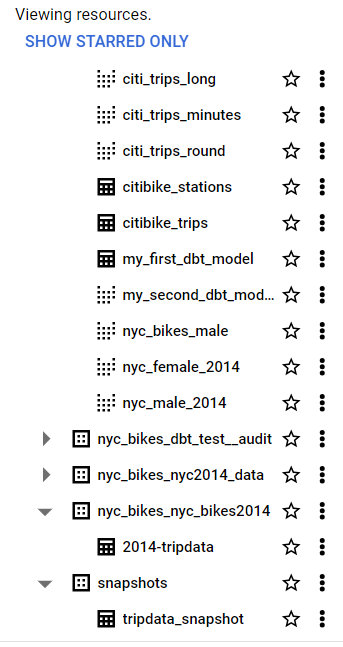
\includegraphics{./images/snapshots_schema.png}
\caption{Snapshots schema}
\end{figure}

When you run \texttt{dbt\ snapshot} the first time, the \texttt{dbt\_valid\_to} column will be \texttt{null} for all records. Thereafter, when you run subsequent \texttt{dbt\ snapshot} executions for a table that has undergone a change, the \texttt{dbt\_valid\_to} will be populated with a timestamp value in the \texttt{dbt\_valid\_to} of the altered row.

\hypertarget{the-check-strategy}{%
\section{\texorpdfstring{The \texttt{check} strategy}{The check strategy}}\label{the-check-strategy}}

Now is the time to truly test if our snapshots work. Go to the SQL tab of your Big Query and insert a new row using this query:

\begin{verbatim}
INSERT INTO `dbt-project-437116`.`nyc_bikes_nyc_bikes2014`.`2014-tripdata` (`_id`, `tripduration`, `start station name`) 
VALUES (000000, 1000, 'Nowhere Near Station');
\end{verbatim}

Thereafter run \texttt{dbt\ snapshot}.

Ensure that the new row has been added by crosschecking its existence via:

\begin{verbatim}
SELECT * FROM `dbt-project-437116`.`nyc_bikes_nyc_bikes2014`.`2014-tripdata`
WHERE `start station name` = 'Nowhere Near Station';
\end{verbatim}

Now check if our \texttt{tripdata\_snapshot} table has captured the new row using the below query.

\begin{verbatim}
SELECT * FROM `dbt-project-437116`.`snapshots`.`tripdata_snapshot`
WHERE `start station name` = 'Nowhere Near Station';
\end{verbatim}

Its a new row of data, which means all columns have been affected with a new value in each. Remember we set the \texttt{check\_cols=all}.

\begin{figure}
\centering
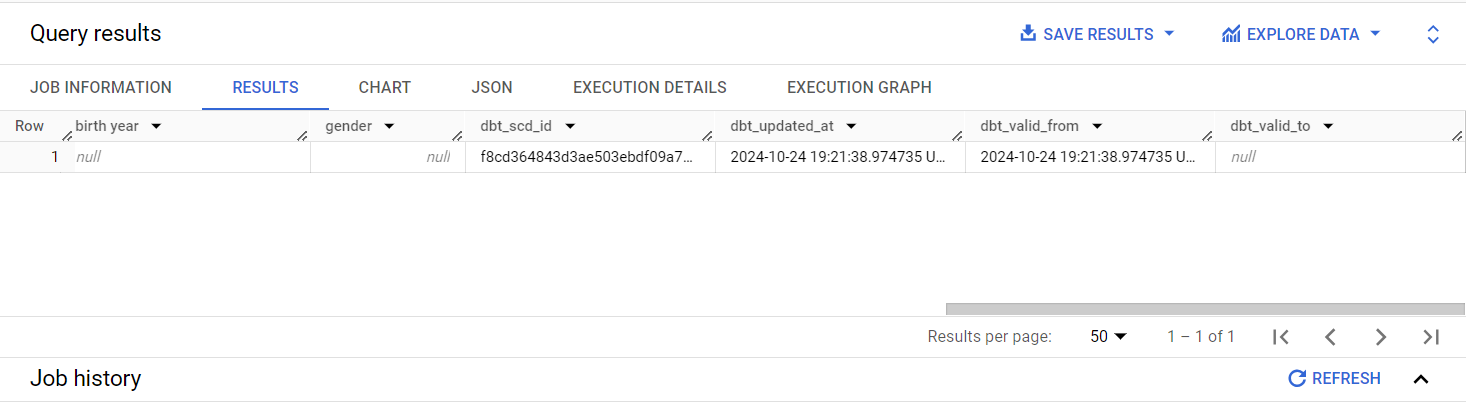
\includegraphics{./images/inserted_new_row.png}
\caption{Recorded change}
\end{figure}

Let's go on.

Insert a new row, with an additional extra change in the \texttt{\_id} column.

\begin{verbatim}
UPDATE `dbt-project-437116`.`nyc_bikes_nyc_bikes2014`.`2014-tripdata`
SET `start station name` = 'Even Further Station', `_id` = 1001995
WHERE `_id` = 0;
\end{verbatim}

Again, run \texttt{dbt\ snapshot}. Always run \texttt{dbt\ snapshot} when your data has received new data update.

Let's check if the new row with two updates has been recorded in our snapshots table.

\begin{verbatim}
SELECT * FROM `dbt-project-437116`.`snapshots`.`tripdata_snapshot`
WHERE `start station name` = 'Even Further Station';
\end{verbatim}

If you run this, you will notice that the \texttt{dbt\_valid\_to} is still \texttt{null}. This could possibly be because we have added a new unique key and thus dbt will still treat this as a new record rather than one which was changed from 0 to 1001995.

Now, update the row with \texttt{\_id} 1001995 using the below SQL query.

\begin{verbatim}
UPDATE `dbt-project-437116`.`nyc_bikes_nyc_bikes2014`.`2014-tripdata`
SET `start station name` = 'Furth East Station'
WHERE `_id` = 1001995;
\end{verbatim}

Now after running \texttt{dbt\ snapshot} , let's see if our snapshot table will have tracked the historical change of \texttt{Even\ Further\ Station} and \texttt{Furth\ East\ Station} of row \texttt{\_id} 1001995. Use the below query to unravel the results.

\begin{verbatim}
SELECT * FROM `dbt-project-437116`.`snapshots`.`tripdata_snapshot`
WHERE `_id` = 1001995;
\end{verbatim}

\begin{figure}
\centering
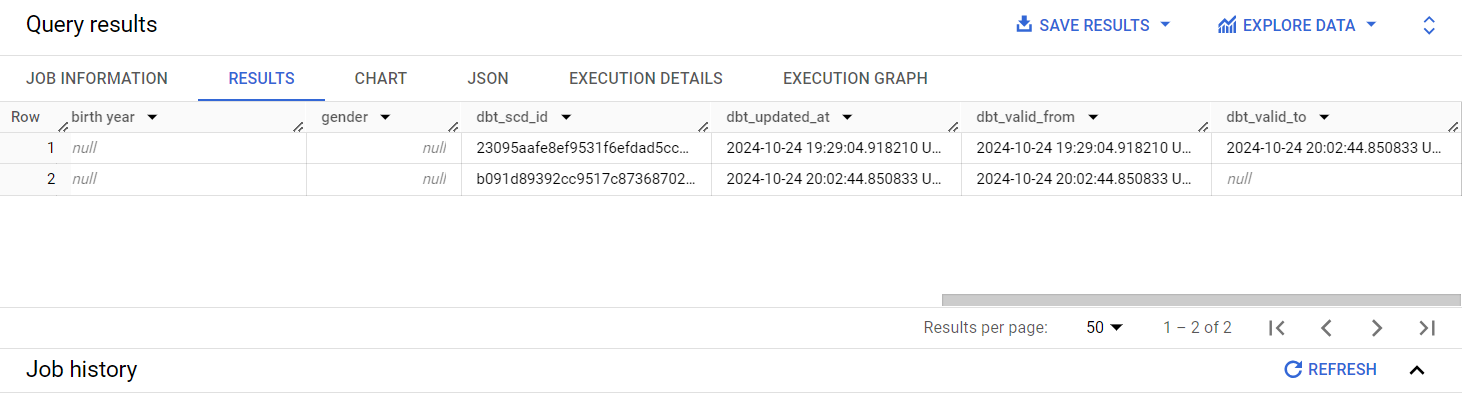
\includegraphics{./images/snapshot_example.png}
\caption{Snapshot example}
\end{figure}

Yes it did! For row 1, which stands for when the `start station name' was \texttt{Even\ Further\ Station}, we can see that row was valid from 2024-10-24 19:29 to 2024-10-24 20:02. However, the new row 2, which is where the `start station name' was switched to \texttt{Furth\ East\ Station}, we can see it became valid from 2024-10-24 20:02; the exact time when row was updated.

You can indeed check if the latest change is in the \texttt{2014-tripdata} table via:

\begin{verbatim}
SELECT * FROM `dbt-project-437116`.`nyc_bikes_nyc_bikes2014`.`2014-tripdata`
WHERE `start station name` = 'Furth East Station';
\end{verbatim}

\hypertarget{the-timestamp-strategy}{%
\section{\texorpdfstring{The \texttt{timestamp} strategy}{The timestamp strategy}}\label{the-timestamp-strategy}}

The \texttt{timestamp} strategy in snapshoting relies on an \texttt{updated\_at} column to check if any changes have occurred on the row. If the configured \texttt{updated\_at} column is more recent than when the table was last run, dbt will invalidate the old record and record a new one. If the timestamps are unchanged, dbt will not take any action.

The \texttt{timestamp} strategy requires an \texttt{updated\_at} column which represents when the row was last updated. In order to work with \texttt{timestamp} strategy, we need to recreate our \texttt{2014-tripdata} but now with an additional \texttt{updated\_at} column. It can be any table, so long as there is an \texttt{updated\_at} column, but we settled on this one because it is lightweight. Plus, we already have it as a seed. We will use a dbt model to recreated the \texttt{2014-tripdata} seed but with an extra \texttt{updated\_at} column.

Create a \texttt{nyc\_bikes\_timestamp} SQL model inside the \texttt{sources} folder. Copy paste the following contents into the model.

\begin{verbatim}
{{ config(
    materialized="table",
    schema="nyc_bikes_nyc_bikes2014"
) }}

WITH nyc_bikes_timestamp AS (
  SELECT *, CURRENT_TIMESTAMP() AS updated_at FROM {{ source('nyc_bikes_nyc_bikes2014', '2014-tripdata') }}
)

SELECT
  *
FROM nyc_bikes_timestamp
\end{verbatim}

\begin{figure}
\centering
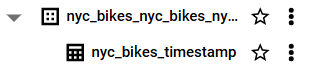
\includegraphics{./images/timestamp_table.png}
\caption{Timestamp table}
\end{figure}

We are configuring it as a table because for some reason, when trying to update fields into this model using BigQuery, an error came up simply because it was a view!

Now run \texttt{dbt\ run\ -\/-select\ sources}. You will get the below output.

\begin{verbatim}
19:08:14  Concurrency: 1 threads (target='dev')
19:08:14  
19:08:14  1 of 4 START sql view model nyc_bikes.nyc_bikes_male ........................... [RUN]
19:08:16  1 of 4 OK created sql view model nyc_bikes.nyc_bikes_male ...................... [CREATE VIEW (0 processed) in 2.45s]
19:08:16  2 of 4 START sql table model nyc_bikes_nyc_bikes_nyc_bikes2014.nyc_bikes_timestamp  [RUN]
19:08:22  2 of 4 OK created sql table model nyc_bikes_nyc_bikes_nyc_bikes2014.nyc_bikes_timestamp  [CREATE TABLE (224.7k rows, 33.3 MiB processed) in 5.31s]
19:08:22  3 of 4 START sql view model nyc_bikes.nyc_female_2014 .......................... [RUN]
19:08:24  3 of 4 OK created sql view model nyc_bikes.nyc_female_2014 ..................... [CREATE VIEW (0 processed) in 2.22s]
19:08:24  4 of 4 START sql view model nyc_bikes.nyc_male_2014 ............................ [RUN]
19:08:26  4 of 4 OK created sql view model nyc_bikes.nyc_male_2014 ....................... [CREATE VIEW (0 processed) in 2.39s]
19:08:26  
19:08:26  Finished running 3 view models, 1 table model in 0 hours 0 minutes and 29.78 seconds (29.78s).
19:08:26  
19:08:26  Completed successfully
19:08:26  
19:08:26  Done. PASS=4 WARN=0 ERROR=0 SKIP=0 TOTAL=4
\end{verbatim}

Now that we have already created a table of \texttt{nyc\_bikes\_timestamp}, we would also want to reference it in downstream models. As you read in an earlier chapter, dbt sources are what make models to be referenced in other queries using the \texttt{source()} function. Therefore in the \texttt{sources/sources\_bikes.yml}, add the following:

\begin{verbatim}
- name: nyc_bikes_nyc_bikes_nyc_bikes2014
        schema: nyc_bikes_nyc_bikes_nyc_bikes2014
        tables:
          - name: nyc_bikes_timestamp
            description: ''
\end{verbatim}

Now is the time to create a dbt snapshot relying on the \texttt{timestamp} strategy.

Create a \texttt{timestamp\_snapshot} in the \texttt{snapshots} directory with the following SQL contents.

\begin{verbatim}


{{
  config(      
    target_schema='snapshots',      
    strategy='timestamp',      
    unique_key='_id',      
    updated_at='updated_at'    
  )  
}}  

SELECT * FROM `dbt-project-437116`.`nyc_bikes_nyc_bikes_nyc_bikes2014`.`nyc_bikes_timestamp`


\end{verbatim}

You may wonder why we are not using something like \texttt{\{\{\ source("schema",\ "table")\ \}\}} in the SELECT statement. We had initially run that with \texttt{nyc\_bikes\_nyc\_bikes\_nyc\_bikes2014} and \texttt{nyc\_bikes\_timestamp} as the \emph{schema} and \emph{table} names respectively. However, dbt kept throwing an error that it couldn't find such a table therefore we resulted in the unorthodox way of hardcoding the entire dataset-schema-table namespace.

Now run \texttt{dbt\ snapshot} to create the \texttt{nyc\_bikes\_timestamp} table.

\begin{verbatim}
19:31:54  Concurrency: 1 threads (target='dev')
19:31:54  
19:31:54  1 of 2 START snapshot snapshots.timestamp_snapshot ............................. [RUN]
19:32:02  1 of 2 OK snapshotted snapshots.timestamp_snapshot ............................. [CREATE TABLE (224.7k rows, 35.0 MiB processed) in 8.10s]
19:32:02  2 of 2 START snapshot snapshots.tripdata_snapshot .............................. [RUN]
19:32:15  2 of 2 OK snapshotted snapshots.tripdata_snapshot .............................. [MERGE (0.0 rows, 44.0 MiB processed) in 12.54s]
19:32:15  
19:32:15  Finished running 2 snapshots in 0 hours 0 minutes and 28.86 seconds (28.86s).
19:32:15  
19:32:15  Completed successfully
19:32:15  
19:32:15  Done. PASS=2 WARN=0 ERROR=0 SKIP=0 TOTAL=2
\end{verbatim}

\begin{figure}
\centering
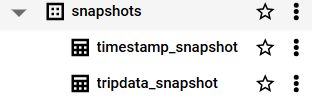
\includegraphics{./images/timestamp_snapshot_created.png}
\caption{Timestamp snapshot}
\end{figure}

Now to check if our timestamp table can snapshot changes, let's insert a new row and make some changes to it. Paste the following in a SQL tab in BigQuery.

\begin{verbatim}
INSERT INTO `dbt-project-437116`.`nyc_bikes_nyc_bikes_nyc_bikes2014`.`nyc_bikes_timestamp` (`_id`, `tripduration`, `start station name`, `updated_at`) 
VALUES (21001995, 2000, 'Sumwhere Near Station', '2024-10-25 23:09:47.169668 UTC');
\end{verbatim}

Note the \texttt{updated\_at} column. Unlike when working with the \texttt{check} strategy which could still work well with several fields as \texttt{null}, omitting the \texttt{updated\_at} column in the \texttt{timestamp} strategy is costly as dbt will be unable to track any change. All you will get is just a new field but with several \texttt{null} values in the snapshot table.

Now run \texttt{dbt\ snapshot} and when it succesfully runs, check \texttt{timestamp\_snapshot} table using this SELECT statement in BigQuery.

\begin{verbatim}
SELECT * FROM `dbt-project-437116`.`snapshots`.`timestamp_snapshot` 
WHERE `_id` = 21001995;
\end{verbatim}

Now change the station name from `Sumwhere Here Station` to 'Somewhere Near Station' to demonstrate tracking a change.

\begin{verbatim}
UPDATE `dbt-project-437116`.`nyc_bikes_nyc_bikes_nyc_bikes2014`.`nyc_bikes_timestamp`
SET `start station name` = 'Somewhere Here Station', `updated_at` = '2024-10-25 23:14:47.169668 UTC'
WHERE `_id` = 21001995;
\end{verbatim}

Run \texttt{dbt\ snapshot}.

Now check if dbt has been able to track changes. We expect that the row with the station name `Sumwhere Near Station' was valid for a short period (see the \texttt{dbt\_valid\_from} and \texttt{dbt\_valid\_to} columns) while the `Somewhere Here Station' is the most current.

\begin{verbatim}
SELECT * FROM `dbt-project-437116`.`snapshots`.`timestamp_snapshot` 
WHERE `_id` = 21001995;
\end{verbatim}

You should see we've been able to track changes.

\begin{figure}
\centering
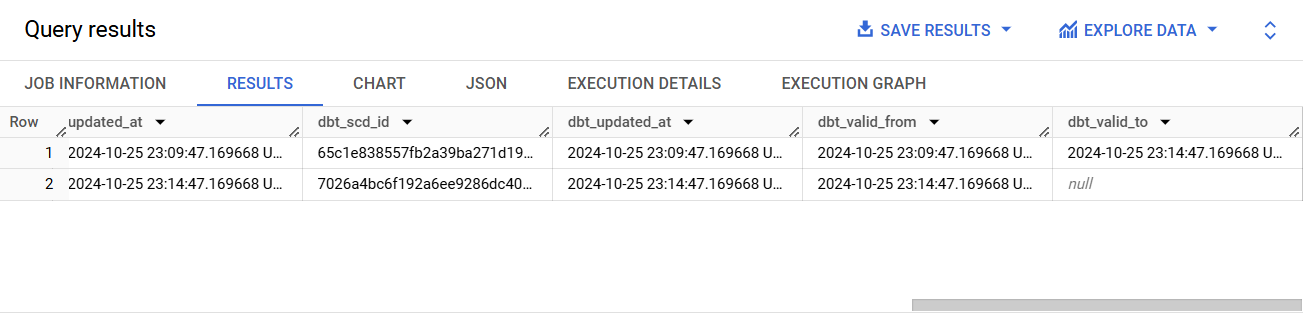
\includegraphics{./images/timestamp_tracking.png}
\caption{Timestamp tracking}
\end{figure}

The downside of using the \texttt{timestamp} strategy is that you have to use the \texttt{updated\_at} column or whatever timestamp column you defined. Nevertheless, based on our exercise so far, the \texttt{check} strategy is far much better and less taxing.

\hypertarget{analyses}{%
\chapter{Analyses}\label{analyses}}

In dbt, analyses are those kind of queries that might not exactly be very much needed as a model but can be used for data exploration and visualization. Typically, any SQL model that is for analytical rather than modeling purposes is stored within the \texttt{analyses} directory. Thereafter, running the code \texttt{dbt\ compile} will create the compiled SQL file inside the \texttt{target/compiled/\{project\ name\}/analyses/sql\_file\_name.sql} directory. The code inside this directory can be pasted in a data visualization tool but it will not appear in the data warehouse. You read that well: it will not.

\hypertarget{creating-an-analysis}{%
\section{\texorpdfstring{Creating an \texttt{analysis}}{Creating an analysis}}\label{creating-an-analysis}}

As mentioned earlier, analyses queries are stored within the \texttt{analysis} folder. To begin with, we shall create a SQL query that performs a join. The below query will join the rows in \texttt{nyc\_bikes\_nyc\_bikes2014}.\texttt{2014-tripdata} with those in \texttt{nyc\_bikes}.\texttt{citi\_trips\_round} based on station id. The aforementioned contents are found within the \texttt{start\_join\_bikes} SQL within the \texttt{analyses} folder.

\begin{verbatim}
WITH `2014-tripdata` AS (
    SELECT * FROM {{ source('nyc_bikes_nyc_bikes2014', '2014-tripdata') }}
), 

WITH citi_trips_round AS (
    SELECT * FROM {{ source('nyc_bikes', 'citi_trips_round') }}
)

SELECT cs.`start station id`, cs.`start station name`, 
ct.bikeid, ct.start_station_id, ct.trip_min_round 
FROM `2014-tripdata` cs 
JOIN citi_trips_round ct 
ON cs.`start station id` = ct.start_station_id
WHERE ct.trip_min_round > 50000
\end{verbatim}

Thereafter type and hit \texttt{dbt\ compile} on the terminal. The results will appear in the \texttt{dbt\_book/target/compiled/dbt\_book/analyses} directory. The query is actually the same, as you can see below. The only exception is that the references within the \texttt{source} file have been expanded to contain the full table path.

\begin{verbatim}
WITH `2014-tripdata` AS (
    SELECT * FROM `dbt-project-437116`.`nyc_bikes_nyc_bikes2014`.`2014-tripdata`
), 

WITH citi_trips_round AS (
    SELECT * FROM `dbt-project-437116`.`nyc_bikes`.`citi_trips_round`
)

SELECT cs.`start station id`, cs.`start station name`, 
ct.bikeid, ct.start_station_id, ct.trip_min_round 
FROM `2014-tripdata` cs 
JOIN citi_trips_round ct 
ON cs.`start station id` = ct.start_station_id
WHERE ct.trip_min_round > 50000
\end{verbatim}

However, pasting this on BigQuery results in the below error.

\begin{figure}
\centering
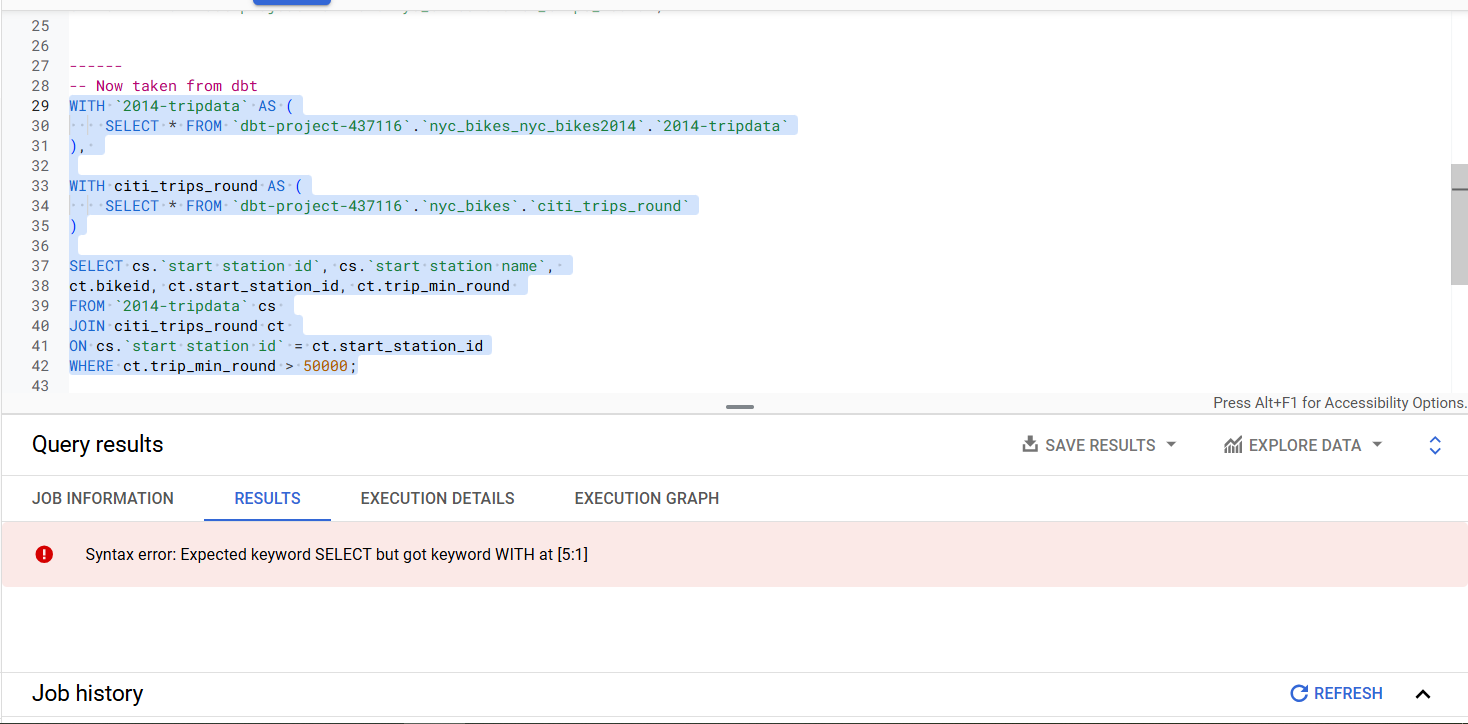
\includegraphics{./images/analyses_error.png}
\caption{Analyses error}
\end{figure}

Therefore, we created a second model which does the same work but without the \texttt{WITH} statement. These are the contents of \texttt{station\_join\_bikes\_snd.sql}.

\begin{verbatim}
SELECT cs.`start station id`, cs.`start station name`, 
ct.bikeid, ct.start_station_id, ct.trip_min_round 
FROM {{ source('nyc_bikes_nyc_bikes2014', '2014-tripdata') }} cs 
JOIN {{ source('nyc_bikes', 'citi_trips_round') }} ct 
ON cs.`start station id` = ct.start_station_id
WHERE ct.trip_min_round > 50000;
\end{verbatim}

The contents of the SQL file inside the \texttt{dbt\_book/target/compiled/dbt\_book/analyses} directory are as follows:

\begin{verbatim}
SELECT cs.`start station id`, cs.`start station name`, 
ct.bikeid, ct.start_station_id, ct.trip_min_round 
FROM `dbt-project-437116`.`nyc_bikes_nyc_bikes2014`.`2014-tripdata` cs 
JOIN `dbt-project-437116`.`nyc_bikes`.`citi_trips_round` ct 
ON cs.`start station id` = ct.start_station_id
WHERE ct.trip_min_round > 50000;
\end{verbatim}

The full table path was expanded and pasting this query into BigQuery produces the results without a fuss.

\hypertarget{definitions-for-analyses}{%
\section{\texorpdfstring{Definitions for \texttt{analyses}}{Definitions for analyses}}\label{definitions-for-analyses}}

The definitions for \texttt{analyses} are created the same way as the other YAML files we have created for other models, only that this time they are within the \texttt{analyses} folder.

\hypertarget{exposures}{%
\chapter{Exposures}\label{exposures}}

Imagine a soldier dropping a piece of paper containing their camp location, trails and military equipment only for it to be picked up by a wandering enemy. That would be catastrophic, right? That is akin to exposing them into the line of fire. However, exposures in dbt serve a good purpose. They show how your data is used by downstream projects, be they be notebooks, a dashboard or another data pipeline. They only thing that sets apart exposures from other models is that this time round you are the one who defines which projects will be used downstream. For example, if you want to show your CEO which models were used to create the dashboard, instead of showing the ten models you sifted through, you only show the three that made it to the dashboard.

\hypertarget{creating-an-exposure}{%
\section{Creating an exposure}\label{creating-an-exposure}}

Exposures are written in YAML files but nested under the \texttt{exposures:} key. Below is an exposure created in the \texttt{exposure/exposures.yml} path.

\begin{verbatim}
version: 2

exposures:

  - name: station_bikes_exposure
    label: A join of station tables and bike rides
    type: dashboard
    maturity: high
    url: https://public-toilets-in-australia-infomap.onrender.com/
    description: '{{ doc("citi_trips_round") }}'

    depends_on:
      - ref('citi_trips_round')
      - ref('citi_trips_minutes') # Added this just to increase complexity of lineage graph
      - source('nyc_bikes_nyc_bikes2014', '2014-tripdata')

    owner:
      name: Mr Fantastic
      email: mrfantastic@unlike.com
\end{verbatim}

Below is the definition of each property used above.

\textbf{Required}

\begin{itemize}
\item
  \texttt{name}: a unique exposure name written in snake case
\item
  \texttt{type}: one of dashboard, notebook, analysis, ml or application
\item
  \texttt{owner}: name or email required; additional properties allowed
\end{itemize}

\textbf{Expected}

\texttt{depends\_on}: list of nodes, including \texttt{metric}, \texttt{ref}, and \texttt{source}. While possible, it is highly unlikely you will ever need an \texttt{exposure} to depend on a \texttt{source} directly.

\textbf{Optional}

\begin{itemize}
\item
  \texttt{label}: May contain spaces, capital letters, or special characters.
\item
  \texttt{url}: Activates and populates the link to View this exposure in the upper right corner of the generated documentation site
\item
  \texttt{maturity}: Indicates the level of confidence or stability in the exposure. One of high, medium, or low. For example, you could use high maturity for a well-established dashboard, widely used and trusted within your organization. Use low maturity for a new or experimental analysis.
\end{itemize}

\textbf{General properties (optional)}

\begin{itemize}
\tightlist
\item
  description
\item
  tags
\item
  meta
\end{itemize}

\hypertarget{running-an-exposure}{%
\section{Running an exposure}\label{running-an-exposure}}

To run the exposure we just created, we use the following one liner. The plus sign is there to indicate to dbt to include all models used to feed into the \texttt{station\_bikes\_exposure} exposure.

\begin{verbatim}
dbt run --select +exposure:station_bikes_exposure
\end{verbatim}

It is noteworthy to mention that you run the \texttt{name} value under the \texttt{exposures} key. The name of the YAML is not used when running exposures.

Here is the output:

\begin{verbatim}
20:31:06  Concurrency: 1 threads (target='dev')
20:31:06  
20:31:06  1 of 2 START sql view model nyc_bikes.citi_trips_minutes ....................... [RUN]
20:31:09  1 of 2 OK created sql view model nyc_bikes.citi_trips_minutes .................. [CREATE VIEW (0 processed) in 3.10s]
20:31:09  2 of 2 START sql view model nyc_bikes.citi_trips_round ......................... [RUN]
20:31:12  2 of 2 OK created sql view model nyc_bikes.citi_trips_round .................... [CREATE VIEW (0 processed) in 2.80s]
20:31:12  
20:31:12  Finished running 2 view models in 0 hours 0 minutes and 13.36 seconds (13.36s).
20:31:12  
20:31:12  Completed successfully
20:31:12  
20:31:12  Done. PASS=2 WARN=0 ERROR=0 SKIP=0 TOTAL=2
\end{verbatim}

One can also decide to test all the upstream models for our exposure. The below code will display test results for all the three models defined by the \texttt{depends\_on} key.

\begin{verbatim}
19:37:44  Concurrency: 1 threads (target='dev')
19:37:44  
19:37:44  1 of 23 START test dbt_expectations_expect_column_max_to_be_between_citi_trips_minutes_trip_duration_min__326000__16  [RUN]
19:37:49  1 of 23 PASS dbt_expectations_expect_column_max_to_be_between_citi_trips_minutes_trip_duration_min__326000__16  [PASS in 5.51s]
19:37:49  2 of 23 START test dbt_expectations_expect_column_max_to_be_between_citi_trips_round_trip_duration_min__326000__16  [RUN]
19:37:53  2 of 23 PASS 
-- snip --
\end{verbatim}

Nevertheless, we remain with visualizing our exposure.

\hypertarget{visualizing-the-exposure}{%
\section{Visualizing the exposure}\label{visualizing-the-exposure}}

Visualizing exposures is as simple as just generating your dbt documentation. This is actually the default way of displaying exposures. It begins with \texttt{dbt\ docs\ generate} and \texttt{dbt\ docs\ serve}. Afterwards, open the dbt documentation static web page in the port number provided. Ours is \texttt{localhost:/8080}.

\begin{figure}
\centering
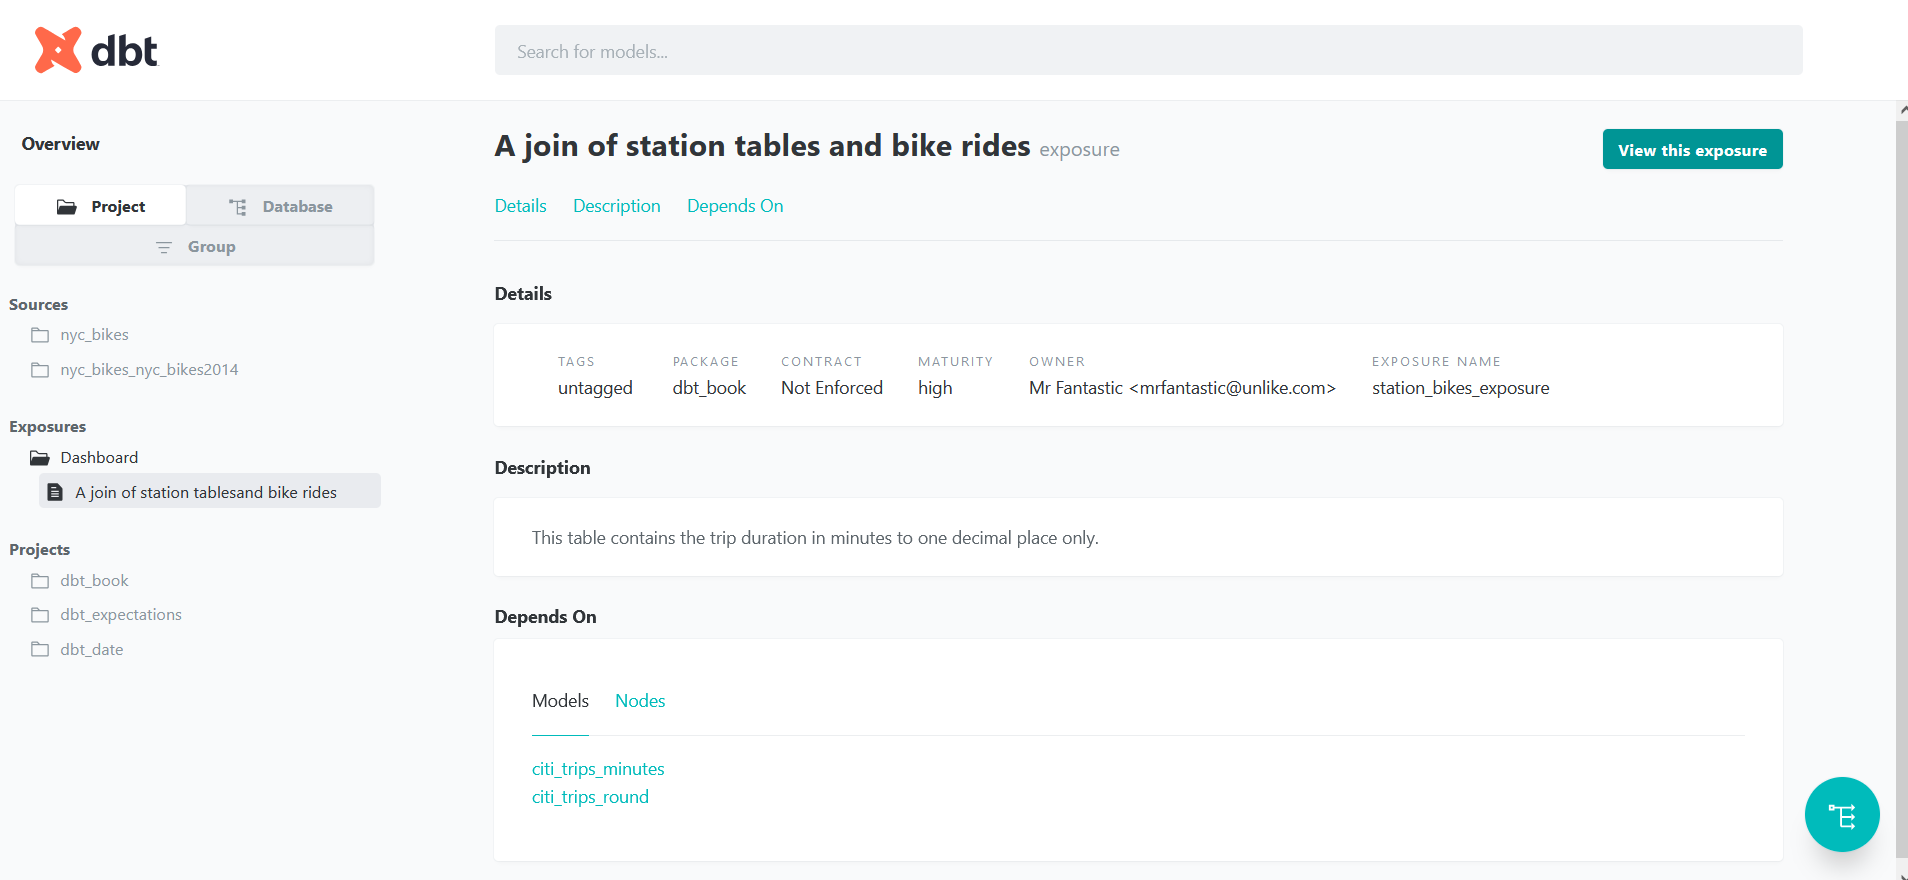
\includegraphics{./images/exposure_webpage.png}
\caption{Exposure}
\end{figure}

You will notice that there is a dedicated section for exposures called \texttt{Exposures}. The exposure title is \texttt{Dashboard} and the label for the exposure is the \texttt{label} value provided in the YAML.

If you click on the blue lineage graph button, you will see the upstream models that feed into our exposure.

\begin{figure}
\centering
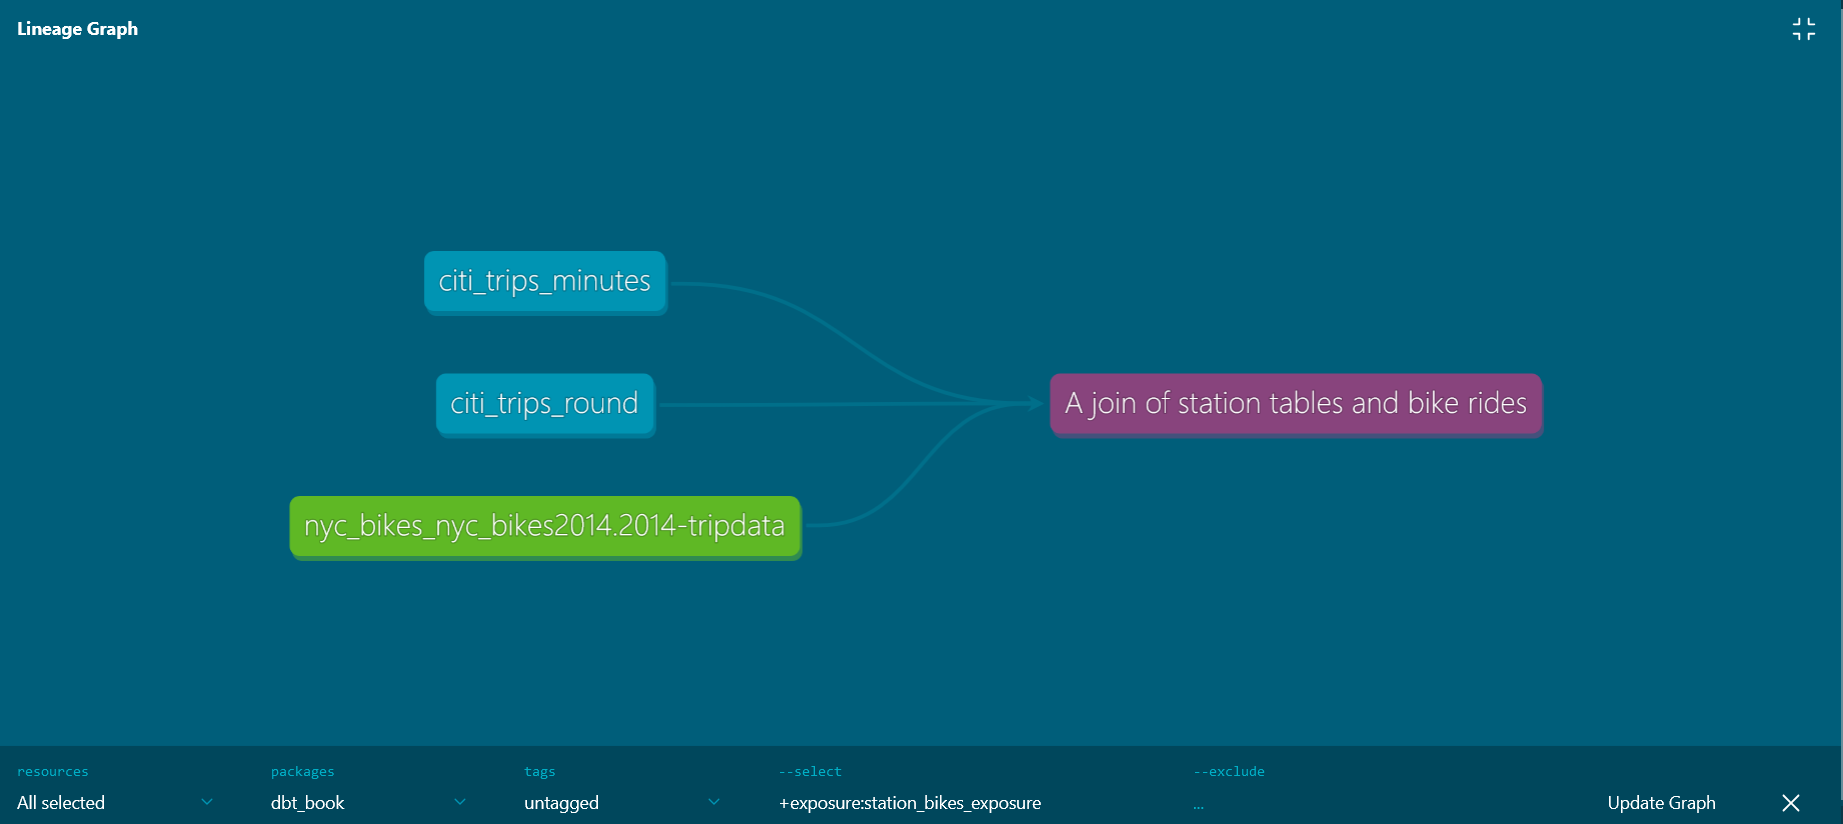
\includegraphics{./images/exposure_lineage_graph.png}
\caption{Exposure lineage graph}
\end{figure}

Still at the bottom of the webpage, the \textbf{Depends on} section contains links to all the upstream models and references for your exposure. Clicking on any takes you to the dbt documentation site for that model.

Finally, there is the \textbf{View this exposure} button. Clicking on it will take you to the url you specified in the \texttt{url:} key of the exposures file. In our case, the url leads to a Dashboard showing all the public sanitation facilities in Australia. Obviously there is no relation between bikes and sanitation facilities. This was just for demonstration purposes only!

\begin{figure}
\centering
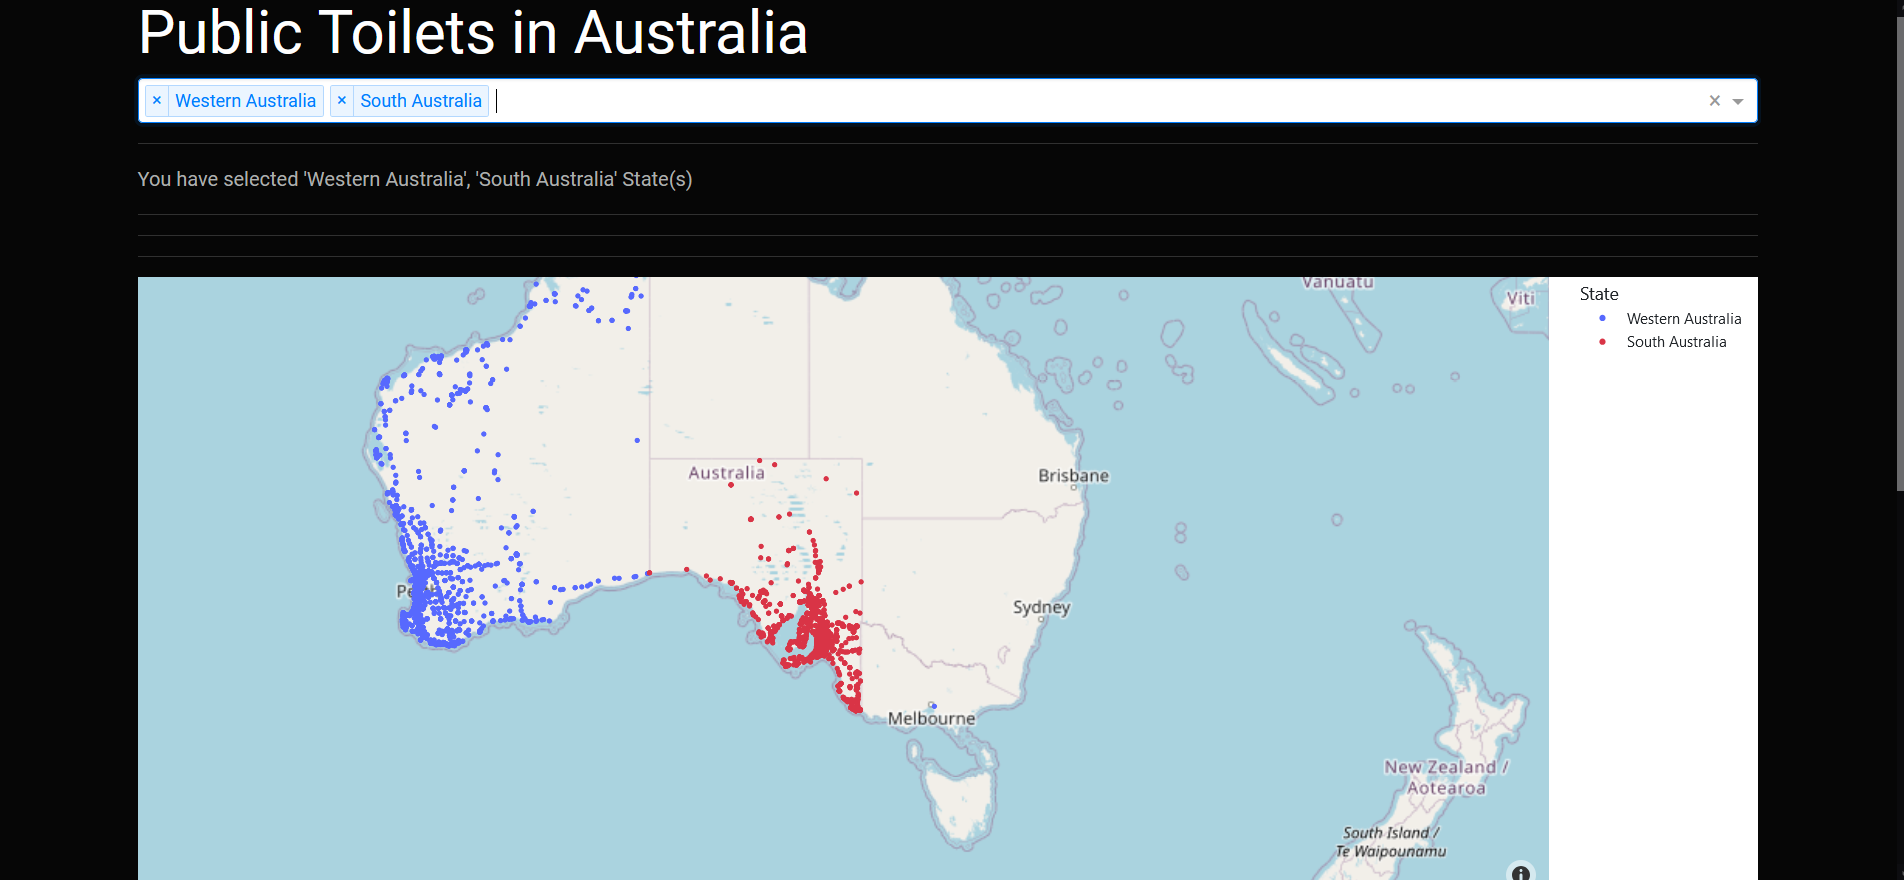
\includegraphics{./images/exposure_hyperlink.png}
\caption{Exposure}
\end{figure}

Working with exposures can be fun. You can add as many exposures as you wish. Below we extended the \texttt{exposures} YAML to also include the following \texttt{station\_bikes\_application} exposure.

\begin{verbatim}
-- snip --
- name: station_bikes_application
    label: An app of stations and bike rides
    type: application
    maturity: high
    url: https://data-visualization-for-diarrhoea-deaths.onrender.com/
    description: '{{ doc("citi_trips_round") }}'

    depends_on:
      - ref('citi_trips_long')
      - ref('citi_trips_minutes') # Added this just to increase complexity of lineage graph
      - source('nyc_bikes_nyc_bikes2014', '2014-tripdata')

    owner:
      name: Mr Fantastic
      email: mrfantastic@unlike.com
\end{verbatim}

Once again, to include this exposure, we run \texttt{dbt\ run\ -\/-select\ +exposure:station\_bikes\_application}. Thereafter create a documentation using the two sesame magic characters of \texttt{dbt\ docs\ generate} and \texttt{dbt\ docs\ serve}.

The above exposure of \texttt{station\_bikes\_application} falls under the \textbf{Application} section as specified in the \texttt{type} key.

\begin{figure}
\centering
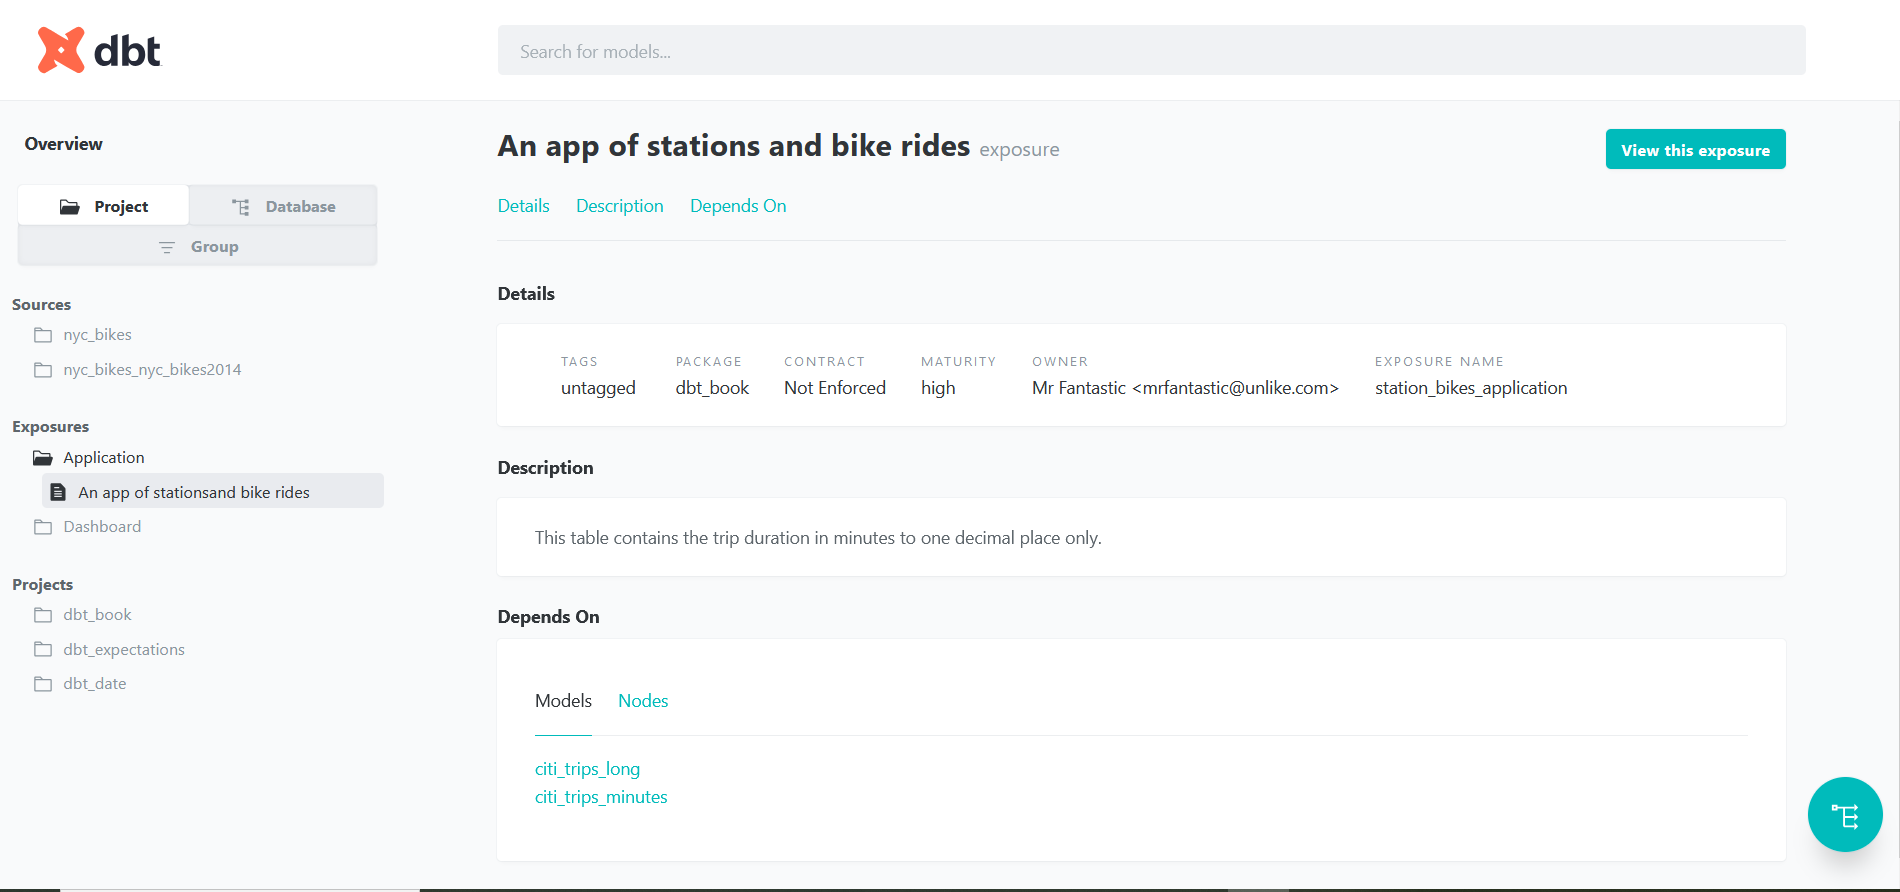
\includegraphics{./images/exposure_application.png}
\caption{Exposure application}
\end{figure}

The lineage graph and the \textbf{View this exposure} buttons work for this exposure as well. In fact this lineage graph is the most complex we've encountered in the course so far. The exposure took into consideration that the \texttt{citi\_trips\_long} model is dependent on the \texttt{citi\_trips\_minutes} and \texttt{citi\_trips\_round} models!

\begin{figure}
\centering
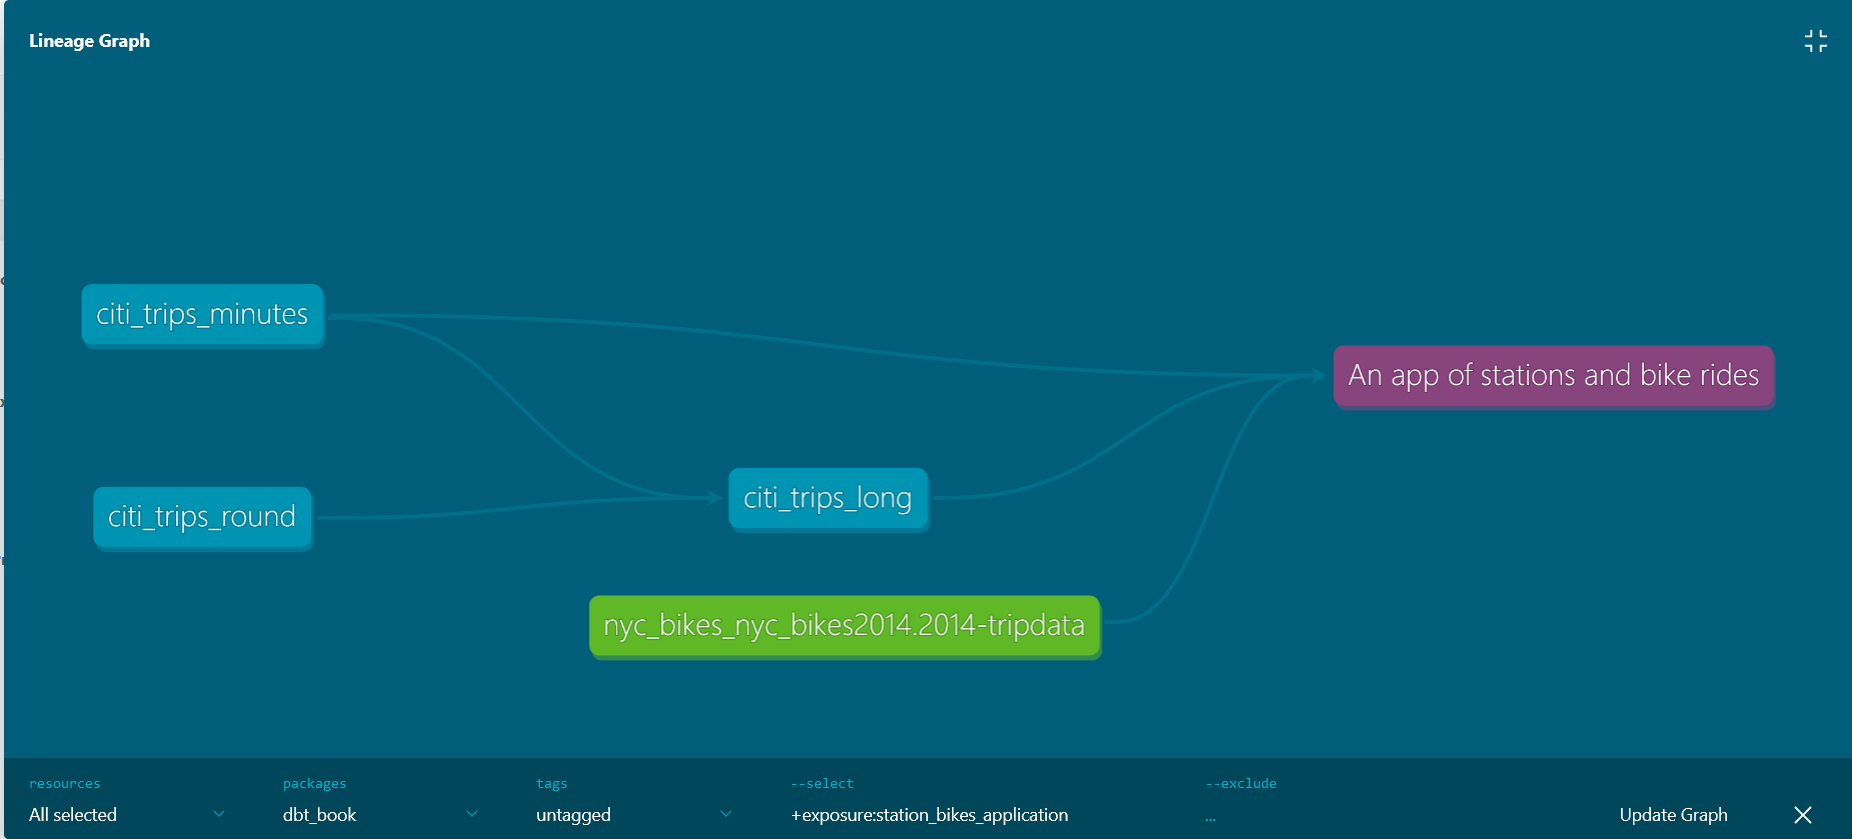
\includegraphics{./images/exposure_lineage_graph2.png}
\caption{Exposure lineage graph}
\end{figure}

The exposure button also leads to a dashboard showing rates of some sanitation related disease. Again, this dashboard is not related to bikes and stations but serves the purpose of demonstration.

\hypertarget{jinja}{%
\chapter{Jinja}\label{jinja}}

\href{https://docs.getdbt.com/docs/build/jinja-macros}{Jinja} in dbt is used to perform functions that regular SQL is unable to do, such as iterating over columns using a \texttt{for} loop and also \texttt{if} statements. Jinja is also used to hold environment variables which can be (re)used all over your project. A simple example of jinja use in dbt is when calling the \texttt{ref()} function. If you see anything with double curly brackets (\texttt{\{\{\ \}\}}) or with brackets and percentage sign(s) in them (\texttt{\{\%\ \%\}}) then you are dealing with jinja.

Let's start by explaining some jinja concepts.

\begin{itemize}
\item
  \textbf{Expressions \{\{ \ldots{} \}\}}: Expressions are used when you want to output a string. You can use expressions to reference variables and call macros.
\item
  \textbf{Statements \{\% \ldots{} \%\}}: Statements don't output a string. They are used for control flow, for example, to set up for loops and if statements, to set or modify variables, or to define macros.
\item
  \textbf{Comments \{\# \ldots{} \#\}}: Jinja comments are used to prevent the text within the comment from executing or outputing a string.
\end{itemize}

Let's start with explaining a \emph{for} loop. This is the skeleton of a \texttt{for} loop in jinja.

\begin{verbatim}

-- SQL Code for {{ item }}

\end{verbatim}

\hypertarget{a-simple-jinja-statement}{%
\section{A simple jinja statement}\label{a-simple-jinja-statement}}

Going by the above cue, let's create a jinja statement that will select all those rows whose bike riders' birth years are any of the following: 1995, 1997 and 2002. Nothing special about these years, just that they stem from the unprofitable notion that they correspond to my birth year and those of my siblings!

Create a new folder called \texttt{jinja} under the \texttt{models} directory and within it create a \texttt{years} SQL file. Copy paste the following contents into \texttt{years.sql}.

\begin{verbatim}



SELECT * 
FROM {{ ref('citi_trips_long') }}
WHERE birth_year = {{ year }}


\end{verbatim}

Let's go through the above line by line.

\begin{itemize}
\item
  \texttt{\{\%\ set\ years\ =\ {[}1995,\ 1997,\ 2002{]}\ \%\}} - this sets the variables we will use to extract some data from our tables. The \texttt{years} variable consists the years that we will use to filter our tables.
\item
  \texttt{\{\%\ for\ year\ in\ years\ \%\}} - the SQL statement that will be repeated is placed inside the \texttt{for\ ...} loop. In this statement, for every year in the \texttt{years} variable list, we will repeat the below sql statement, where \texttt{\{\{\ year\ \}\}} is each year in the \texttt{years} variable:
\end{itemize}

\begin{verbatim}
SELECT * 
FROM {{ ref('citi_trips_long') }}
WHERE birth_year = {{ year }}
\end{verbatim}

\begin{itemize}
\tightlist
\item
  \texttt{\{\%\ endfor\ \%\}} - nothing more than marking the end of the for loop.
\end{itemize}

Now, if we run the code \texttt{dbt\ compile\ -\/-select\ jinja}, you will see a new \texttt{years.sql} appear under the \texttt{target/compiled/dbt\_book/models/jinja/} directory.

Here is how the code looks like:

\begin{verbatim}
SELECT * 
FROM `dbt-project-437116`.`nyc_bikes`.`citi_trips_long`
WHERE birth_year = 1995



SELECT * 
FROM `dbt-project-437116`.`nyc_bikes`.`citi_trips_long`
WHERE birth_year = 1997



SELECT * 
FROM `dbt-project-437116`.`nyc_bikes`.`citi_trips_long`
WHERE birth_year = 2002
\end{verbatim}

What the \texttt{for} loop did was to avoid the redundancy of selecting each \texttt{birth\_year} in its own \texttt{SELECT} statement. Instead it put the three \texttt{SELECT} statements inside one \texttt{for} loop statement. Going a step further, also the redundancy of hardcoding the \texttt{year} is removed. This formula, though a bit complicated, toes in line with the Do not Repeat Yourself (DRY) principle in programming.

\hypertarget{a-more-complex-jinja-query}{%
\section{A more complex jinja query}\label{a-more-complex-jinja-query}}

One can also create more complex jinja queries that leverage other SQL functionalities such as aggregation and CASE WHEN statements. Now suppose, for purely selfish reasons, this author wants to compare the bike ride durations against those of other people who were born in the years 1995, 1997 and 2002. Below is an \texttt{age.sql} file that creates a table that has a column showing the trip duration for each value in the \texttt{years} variable.

\begin{verbatim}


SELECT birth_year, 

SUM (CASE WHEN birth_year = {{ year }} THEN trip_min_round ELSE 0 END) AS trip_min_round_{{ year }},

SUM(trip_min_round) AS totals_trip_min_round
FROM {{ ref('citi_trips_long') }}
GROUP BY birth_year
\end{verbatim}

In the corresponding \texttt{age.sql} in the \texttt{target} directory, this is the compiled SQL query result.

\begin{verbatim}
SELECT birth_year, 

SUM(CASE WHEN birth_year = 1995 THEN trip_min_round ELSE 0 END) AS trip_min_round_1995,

SUM(CASE WHEN birth_year = 1997 THEN trip_min_round ELSE 0 END) AS trip_min_round_1997,

SUM(CASE WHEN birth_year = 2002 THEN trip_min_round ELSE 0 END) AS trip_min_round_2002,

SUM(trip_min_round) AS totals_trip_min_round
FROM `dbt-project-437116`.`nyc_bikes`.`citi_trips_long`
WHERE birth_year IN (
  
  
    1995, 
  
  
    1997, 
  
  
    2002
  
)
GROUP BY birth_year
\end{verbatim}

Pasting this query in BigQuery gives us the below table:

\begin{figure}
\centering
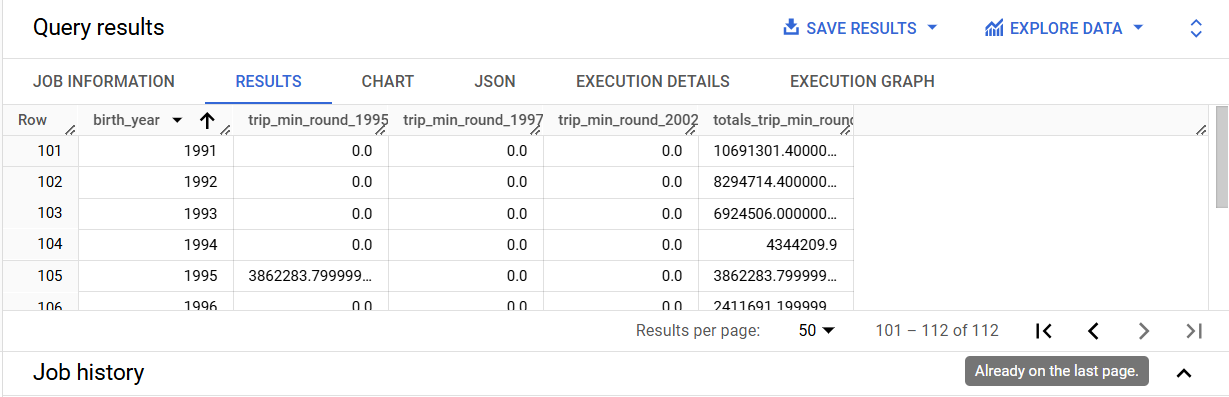
\includegraphics{./images/age_query.png}
\caption{Age query}
\end{figure}

We can see a column for trip duration in minutes for each of the three select years of 1995, 1997 and 2002. However, other years not set in our \texttt{years} variable are included as well, but with the value \texttt{0} in each of the three columns. Before one starts getting confused and blaming the universe for not wanting us to succeed, there is a way we can sort this pesky issue: enter the \texttt{if\ not\ loop.last} statement!

In our previous SQL query, you saw that one can sort the issue of excluding unnecessary years using the \texttt{WHERE} clause. For example, we would have used the clause \texttt{WHERE\ birth\_year\ IN\ (1995,\ 1997,\ 2002)}. However, we frowned on this approach because it is breaking the DRY principle by hardcoding the years by hand. Taking a more complex approach to fulfil the DRY principle sounds like we are exhibiting Obsessive Compulsive Disorder (OCD) but being obsessed in doing things in a higher way is not all too bad in programming.

The \href{https://docs.y42.com/docs/how-to-use-jinja}{\texttt{if\ not\ loop.last} statement} separates the values of interest with a comma, thus effectively fulfilling the work the \texttt{WHERE} clause where it failed. The \texttt{age2.sql} shows this in action.

\begin{verbatim}


SELECT birth_year, 

SUM(CASE WHEN birth_year = {{ year }} THEN trip_min_round ELSE 0 END) AS trip_min_round_{{ year }},

SUM(trip_min_round) AS totals_trip_min_round
FROM {{ ref('citi_trips_long') }}
WHERE birth_year IN (
  
  {# this will separate the years 1995, 1997 and 2002 with a comma, nothing out of this world #}
    {{ year }}, 
  
)
GROUP BY birth_year
\end{verbatim}

Running the \texttt{dbt\ compile\ -\/-select\ jinja} code will compile the \texttt{age2.sql} inside the \texttt{target} directory. It's contents are as follows. Notice the effect of the \texttt{if\ not\ loop.last} statement at the end and how it is a replicate of hardcoding \texttt{WHERE\ birth\_year\ IN\ (1995,\ 1997,\ 2002)}.

\begin{verbatim}
SELECT birth_year, 

SUM(CASE WHEN birth_year = 1995 THEN trip_min_round ELSE 0 END) AS trip_min_round_1995,

SUM(CASE WHEN birth_year = 1997 THEN trip_min_round ELSE 0 END) AS trip_min_round_1997,

SUM(CASE WHEN birth_year = 2002 THEN trip_min_round ELSE 0 END) AS trip_min_round_2002,

SUM(trip_min_round) AS totals_trip_min_round
FROM `dbt-project-437116`.`nyc_bikes`.`citi_trips_long`
WHERE birth_year IN (
  
  
    1995, 
  
  
    1997, 
  
  
    2002
  
)
GROUP BY birth_year
\end{verbatim}

Copy pasting the above compiled SQL into BigQuery you get a cleaner table with all the other birth years left out.

\begin{figure}
\centering
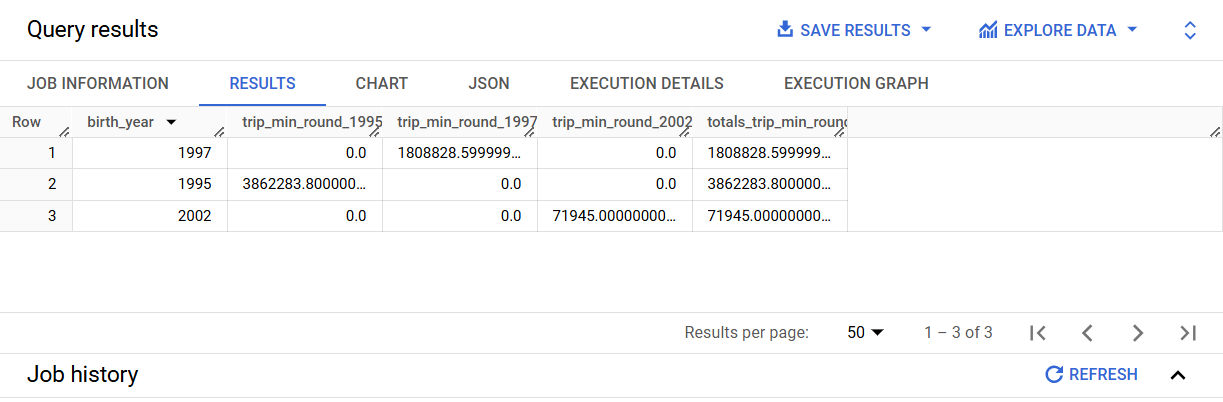
\includegraphics{./images/age2_query.png}
\caption{Age2 query}
\end{figure}

\hypertarget{improvising-using-dry-principle}{%
\section{Improvising using DRY Principle}\label{improvising-using-dry-principle}}

We can go a step further and make our table leaner, by eliminating all the \texttt{trip\_min\_round\_\textless{}year\textgreater{}} columns and having just one \texttt{trip\_min\_round} summation column for the three years 1995, 1997 and 2002. The \texttt{ages3.sql} exemplifies this.

\begin{verbatim}


SELECT birth_year, 
SUM(trip_min_round) AS totals_trip_min_round
FROM {{ ref('citi_trips_long') }}
WHERE birth_year IN (
  
  {# this will separate the years 1995, 1997 and 2002 with a comma, nothing out of this world #}
    {{ year }}, 
  
)
GROUP BY birth_year
\end{verbatim}

After running \texttt{dbt\ compile\ -\/-select\ jinja}, the compiled \texttt{age3.sql} in the target directory is as follows:

\begin{verbatim}
SELECT birth_year, 
SUM(trip_min_round) AS totals_trip_min_round
FROM `dbt-project-437116`.`nyc_bikes`.`citi_trips_long`
WHERE birth_year IN (
  
  
    1995, 
  
  
    1997, 
  
  
    2002
  
)
GROUP BY birth_year
\end{verbatim}

For sure you get a leaner table which is far less verbose.

\begin{figure}
\centering
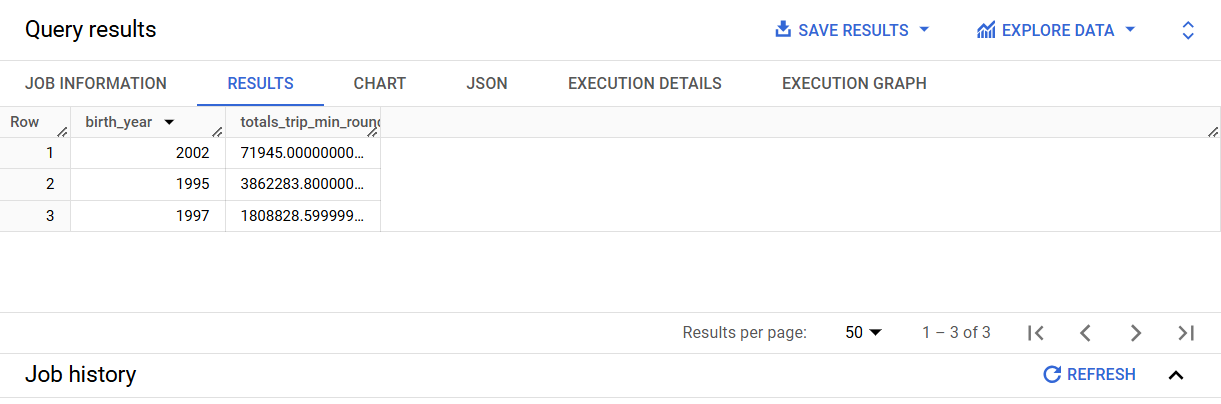
\includegraphics{./images/age3_query.png}
\caption{Age3 query}
\end{figure}

One more thing, you can create views from the SQL jinja queries by simply running the trusty \texttt{dbt\ run\ -\/-select\ jinja}. This is the resulting output.

\begin{verbatim}

--snip--
10:37:54  1 of 4 START sql view model nyc_bikes.age ...................................... [RUN]
10:37:59  1 of 4 OK created sql view model nyc_bikes.age ................................. [CREATE VIEW (0 processed) in 4.98s]
10:37:59  2 of 4 START sql view model nyc_bikes.age2 ..................................... [RUN]
10:38:04  2 of 4 OK created sql view model nyc_bikes.age2 ................................ [CREATE VIEW (0 processed) in 4.26s]
10:38:04  3 of 4 START sql view model nyc_bikes.age3 ..................................... [RUN]
10:38:06  3 of 4 OK created sql view model nyc_bikes.age3 ................................ [CREATE VIEW (0 processed) in 2.77s]
10:38:06  4 of 4 START sql view model nyc_bikes.years .................................... [RUN]
10:38:09  BigQuery adapter: https://console.cloud.google.com/bigquery?project=dbt-project-437116&j=bq:africa-south1:ed8f842b-8077-418b-8222-f5e4cb9438d3&page=queryresults
10:38:09  4 of 4 ERROR creating sql view model nyc_bikes.years ........................... [ERROR in 2.78s]
10:38:09  
10:38:09  Finished running 4 view models in 0 hours 0 minutes and 23.66 seconds (23.66s).
10:38:09  
10:38:09  Completed with 1 error and 0 warnings:
10:38:09  
10:38:09    Database Error in model years (models/jinja/years.sql)
  Syntax error: Expected end of input but got keyword SELECT at [15:1]
  compiled code at target/run/dbt_book/models/jinja/years.sql
  
--snip--
\end{verbatim}

The same views can be called out in BigQuery like the \texttt{age3} view shown below.

\begin{figure}
\centering
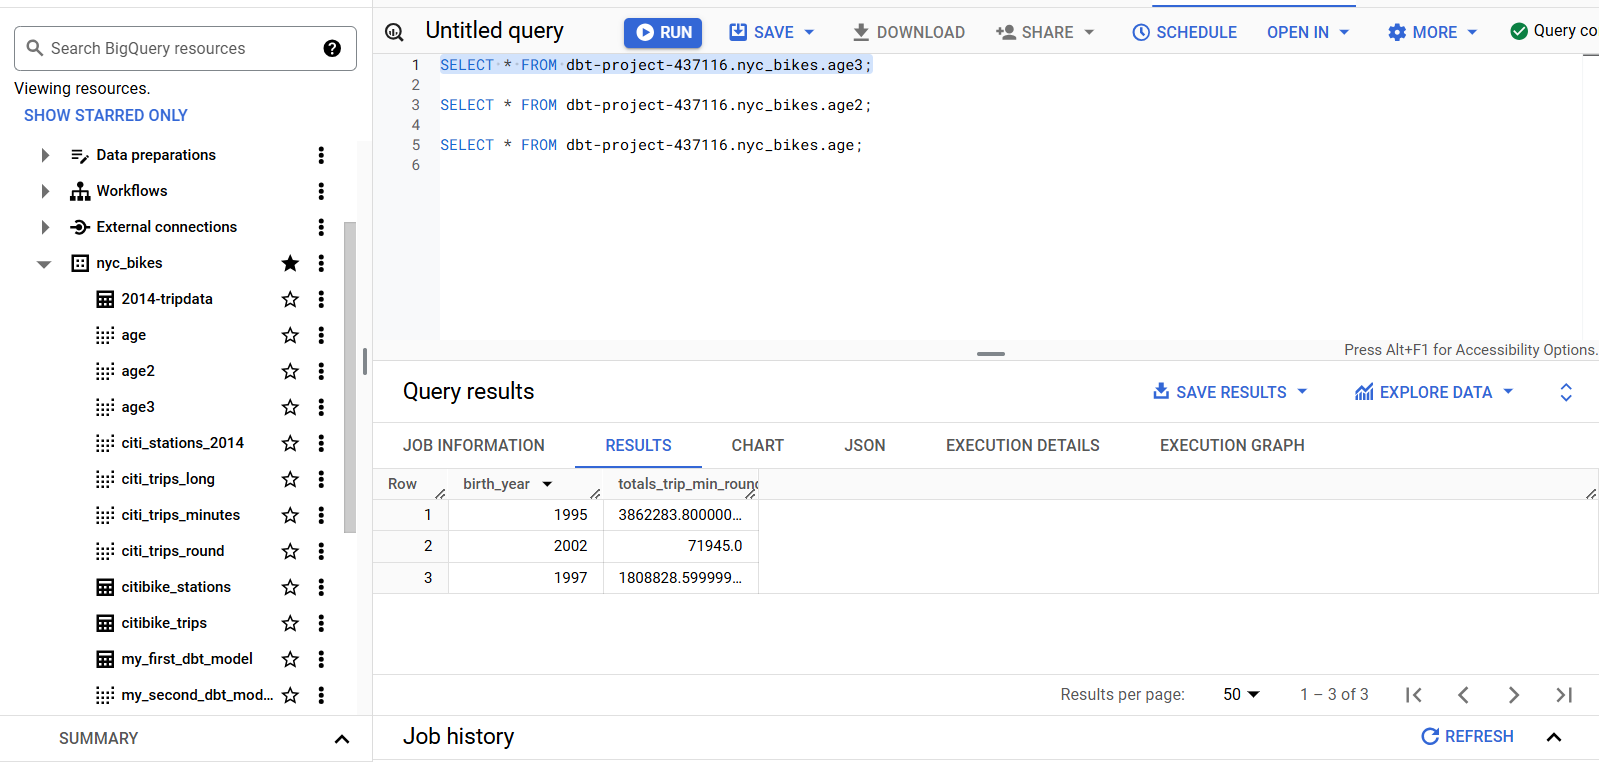
\includegraphics{./images/age3_bigquery.png}
\caption{Age3 view in bigquery}
\end{figure}

Now that the \texttt{\{\%\ if\ not\ loop.last\ \%\}} and its closing \texttt{\{\%\ endif\ \%\}} statements have ceased being cryptic, we can now sort out why the \texttt{years} view could not be created as seen in this \texttt{dbt\ run\ -\/-select\ jinja} error.

\begin{verbatim}
10:38:09  4 of 4 ERROR creating sql view model nyc_bikes.years ........................... [ERROR in 2.78s]
\end{verbatim}

If you look at the compiled SQL for the \texttt{years.sql} in the target directory, there are multiple SELECT statements each for a single year in the \texttt{years} variable. All those three SELECT statements cannot be run simoultaneously to produce a single table in BigQuery. But tweaking the \texttt{jinja/years.sql} a bit and using the \texttt{loop.last} statement will make all the difference. Here is the \texttt{jinja/years2.sql}.

\begin{verbatim}




SELECT * 
FROM {{ ref('citi_trips_long') }}

WHERE birth_year IN (
    
    
    {{ year }}
    ,
    

)
\end{verbatim}

The \texttt{for} loop begins when we want to specify the years, the \texttt{if\ not\ loop} programmatically adds a comma until the last one and finally the \texttt{endfor} statement tells our computer to break out of the looping. Here is the corresponding compiled SQL in the \texttt{years2.sql} in the target directory. When this query is pasted, into BigQuery, it only filters the rows matching to the specified birth years.

\begin{verbatim}
SELECT * 
FROM `dbt-project-437116`.`nyc_bikes`.`citi_trips_long`

WHERE birth_year IN (
    
    
    1995
    ,
    
    
    1997
    ,
    
    
    2002
    
    

)
\end{verbatim}

\begin{figure}
\centering
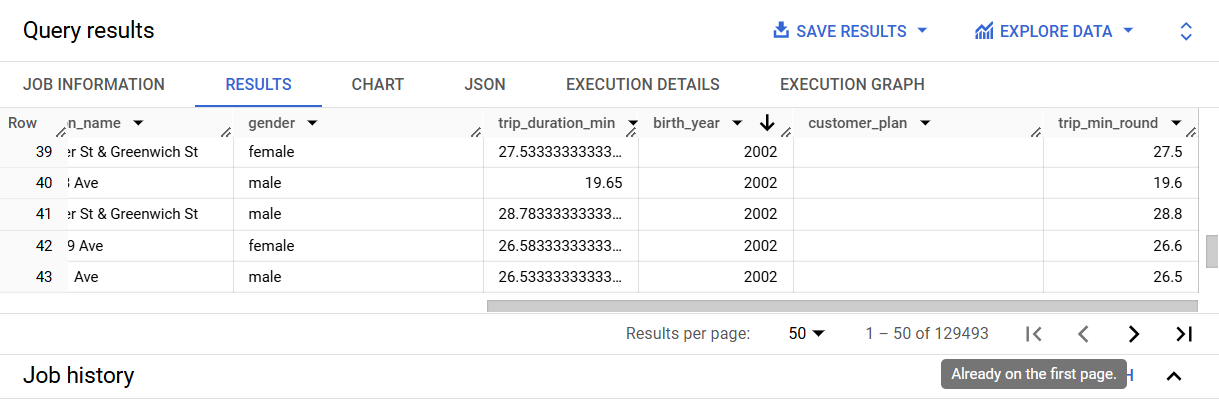
\includegraphics{./images/years2_query.png}
\caption{Years 2 query}
\end{figure}

When we run \texttt{dbt\ run\ -\/-select\ jinja}, this time round the \texttt{years2} view is created.

\begin{verbatim}
--snip--
11:45:10  5 of 5 START sql view model nyc_bikes.years2 ................................... [RUN]
11:45:12  5 of 5 OK created sql view model nyc_bikes.years2 .............................. [CREATE VIEW (0 processed) in 2.29s]
--snip--
\end{verbatim}

\hypertarget{macros}{%
\chapter{Macros}\label{macros}}

A \href{https://www.phdata.io/blog/what-are-dbt-macros/?utm_source=pocket_saves}{macro} in dbt is a reusable piece of code. That's it. A macro in dbt is what a function is to Python or JavaScript. The building block of a macro is the jinja template. Below is the structure of a dbt macro.

\begin{verbatim}


    SQL logic here, using the parameters as needed.


\end{verbatim}

You begin a macro with the name \texttt{macro} and end it with \texttt{endmacro}. Macros are defined in SQL files and stored inside the already shipped \texttt{macros} folder in dbt.

\hypertarget{invoking-a-macro}{%
\section{Invoking a macro}\label{invoking-a-macro}}

There are three ways to call a macro. They are:

\begin{enumerate}
\def\labelenumi{\arabic{enumi}.}
\item
  Using expression blocks
\item
  Call blocks
\item
  Run operation command
\end{enumerate}

\hypertarget{invoking-a-macro-using-expression-blocks}{%
\subsection{Invoking a macro using expression blocks}\label{invoking-a-macro-using-expression-blocks}}

If the macro does not have any parameters, it can be invoked as a solo object like so:

\begin{verbatim}
{{ macro_name() }}
\end{verbatim}

But if it has parameters, we have to call it with it's entire entourage.

\begin{verbatim}
{{ macro_name(arg1, arg2, argN) }}
\end{verbatim}

\hypertarget{invoke-a-macro-using-call-blocks}{%
\subsection{Invoke a macro using call blocks}\label{invoke-a-macro-using-call-blocks}}

In this method, one can invoke a macro inside another macro. Here is the template.

\begin{verbatim}


    Code to be accessed by the macro called_macro


\end{verbatim}

The above code calls a macro called \texttt{called\_macro} and everything in between the \texttt{\{\ \%call\%\ \}} and \texttt{\{\%\ endcall\ \%\}} statements can be accessed using the \texttt{caller()} method.

Here is an example of a macro.

\begin{verbatim}


    SELECT *
    FROM {{ table_name }}
    WHERE {{ caller() }}


\end{verbatim}

Now, call the macro using call blocks.

\begin{verbatim}


CREATE_DATE >= '2020-02-18'::DATE


\end{verbatim}

When it is called it would render:

\begin{verbatim}
SELECT *
FROM EVENT_TABLE
WHERE CREATE_DATE >= '2020-02-18'::DATE
\end{verbatim}

\hypertarget{invoke-a-macro-from-the-command-line-interface-cli}{%
\subsection{Invoke a macro from the Command Line Interface (CLI)}\label{invoke-a-macro-from-the-command-line-interface-cli}}

To run a macro from the CLI or terminal, we use the \texttt{dbt\ run-operation\ \{macro\}\ -\/-args\ \textquotesingle{}\{args\}\textquotesingle{}\{macro\}:} command. The macro will run with the arguments provided. The below macro being run from the CLI selects all columns from a table called \texttt{my\_table}.

\begin{verbatim}
dbt run-operation select_all_columns --args '{table_name: my_table}'
\end{verbatim}

The above are ways to invoke a macro but for simplicity purposes, we shall rely on the first method of invoking macros using expressions.

\hypertarget{simple-macro}{%
\section{Simple macro}\label{simple-macro}}

Having known that a macro acts like a function, let's create a macro that calculates the age of a bike rider. We already have the \texttt{birth\_year} column, so calculating one's age should be as simple as subtracting their birth year from the current year.

As earlier mentioned, macros should go into the \texttt{macros} folder. Create a \texttt{calculate\_age} SQL file and inside it paste the following contents.

\begin{verbatim}


(EXTRACT( YEAR FROM CURRENT_DATE() ) - {{ year }}) 


\end{verbatim}

Remember, a macro is a function and thus what goes within the \texttt{\{\%\ macro\ \%\}} and \texttt{\{\%\ endmacro\ \%\}} expressions is the function itself! This explains why our \texttt{calculate\_age} macro is so succinct. The \texttt{(EXTRACT(\ YEAR\ FROM\ CURRENT\_DATE()\ )\ -\ \{\{\ year\ \}\})} is just SQL's way of extracting the current year and subtracting an earlier year being referenced by the variable \texttt{\{\{\ year\ \}\}}. Of course the specified \texttt{\{\{\ year\ \}\}} column has to be numeric.

Alright. To see the \texttt{calculate\_age} macro in action, create a \texttt{biker\_age} SQL file inside the \texttt{jinja} directory. Paste the following content.

\begin{verbatim}
SELECT *, 
{{ calculate_age("birth_year")}} AS AGE
FROM 
{{ ref('citi_trips_long') }}
\end{verbatim}

In the sub-chapter of \protect\hyperlink{ux5cux23Invokingux5cux2520aux5cux2520macro}{Invoking a Macro}, we saw that a macro is invoked in the following format: \texttt{\{\{\ macro\_name(arg1,\ arg2,\ argN)\ \}\}}. The macro name goes first, followed by the arguments in brackets. We have essentially done this in the \texttt{biker\_age} SQL file. The \texttt{calclate\_age()} macro has been provided the column to calculate on, the \texttt{birth\_year} column. We use the \texttt{AS} keyword to create a new column with the alias \texttt{AGE}. Thereafter, we run the open sesame command \texttt{dbt\ compile\ -\/-select\ macros}.

After compilation, dbt created a \texttt{biker\_age} SQL file containing the below code:

\begin{verbatim}
SELECT *, 


(EXTRACT( YEAR FROM CURRENT_DATE() ) - birth_year) 

 AS AGE
FROM 
`dbt-project-437116`.`nyc_bikes`.`citi_trips_long`
\end{verbatim}

The above should definitely result in a table with the \texttt{AGE} column at the far end.

\hypertarget{complex-macro}{%
\section{Complex macro}\label{complex-macro}}

The above was a simple macro that neatly drove the point home. How about a more complex macro, like one that works on an entire table, transforms it, has more than one argument and oh my\ldots{} one in which you can specify the parameters? We want to write our functions on sand, not stone, so that we can change at will. That's the kind of macro we need.

Let's go. Create a SQL called \texttt{age\_trips} with the following code:

\begin{verbatim}


SELECT {{ column }}, 
SUM({{ duration }}) AS totals_trip_min_round
FROM {{ ref( table_name ) }}
WHERE {{ column }} IN (
  
  {# this will separate the years 1995, 1997 and 2002 with a comma, nothing out of this world #}
    {{ year }}, 
  
)
GROUP BY {{ column }}
ORDER BY {{ column }} DESC


\end{verbatim}

Our intelligent mind (no pun intended) created a macro that selects a column, sums the time duration in that column and additionally, aggregates the sum based on certain numerical column values. It will not sum everything in the entire set but just certain values specified by the \texttt{years} variable. Additionally, we have preset the values to go into the \texttt{years} variables which are \texttt{1995}, \texttt{1997} and \texttt{2002}. Finally, we order the table by arranging the values of the specified columns in descending order.

Now is time to test our macro. Under the \texttt{jinja} directory, create a SQL file called \texttt{age\_trip\_totals}. It should have the below minutiae code.

\begin{verbatim}
{{ age_trips(column='birth_year', duration='trip_min_round',
table_name='citi_trips_long', years = [1990, 1996, 1998, 2001, 2002]) }}
\end{verbatim}

What on earth just happened here? There was no \texttt{SELECT} statement as in the \texttt{biker\_age} file? Yes, there wasn't, and for a good reason. We had already specifed our \texttt{SELECT} blueprint in the macros file. Therefore, calling the \texttt{age\_trips} function from within \texttt{age\_trips\_totals} file will invoke the SQL statement encapsulated by the \texttt{age\_trips} function. If you run \texttt{dbt\ compile\ -\/-select\ macros}, the following SQL file will be compiled in the target directory.

\begin{verbatim}
SELECT birth_year, 
SUM(trip_min_round) AS totals_trip_min_round
FROM `dbt-project-437116`.`nyc_bikes`.`citi_trips_long`
WHERE birth_year IN (
  
  
    1990, 
  
  
    1996, 
  
  
    1998, 
  
  
    2001, 
  
  
    2002
  
)
GROUP BY birth_year
ORDER BY birth_year DESC
\end{verbatim}

Pasting this query on BigQuery will give us a table which aggregates the total trip duration for bikers born in specific years only. That is, those bikers born in any of the following years: 1990, 1996, 1998, 2001 and 2002.

\includegraphics{./images/age_trip.png}
One can also create a view of this macro model using \texttt{dbt\ run\ -\/-select\ age\_trip\_totals}. A \texttt{biker\_age} view should appear under the \texttt{nyc\_bikes} dataset.

By doing the above, we not only created a macros with default parameters, but we could also change them and get valid results. We can do this by tweaking the \texttt{years} argument in our \texttt{age\_trips()} function. As a matter of fact, the \texttt{years} parameter doesn't have to take \emph{years} per se, it can actually work with any numerical column. But we just specified the name \texttt{years} as a clue. In the \texttt{age\_trip\_totals2} SQL file, we specified the ages of interest from within the \texttt{AGE} column of our \texttt{biker\_age} view.

\begin{verbatim}
{{ age_trips(column='AGE', duration='trip_min_round',
table_name='biker_age', years = [22, 27, 29]) }}
\end{verbatim}

Now let's compile this model and see the result:

\begin{verbatim}
dbt compile --select age_trip_totals2
\end{verbatim}

We get the following output in our terminal and by extension, the \texttt{age\_trip\_totals2} SQL file under the \texttt{target} directory.

\begin{verbatim}
19:53:44  Concurrency: 1 threads (target='dev')
19:53:44  
19:53:44  Compiled node 'age_trip_totals2' is:


SELECT AGE, 
SUM(trip_min_round) AS totals_trip_min_round
FROM `dbt-project-437116`.`nyc_bikes`.`biker_age`
WHERE AGE IN (
  
  
    22, 
  
  
    27, 
  
  
    29
  
)
GROUP BY AGE
ORDER BY AGE DESC
\end{verbatim}

Pasting the above in BigQuery gives us an aggregation of the total trip duration for people aged 29, 27 and 22.

\begin{figure}
\centering
\includegraphics{./images/age_trip_totals2.png}
\caption{Age trip total 2 view}
\end{figure}

As mentioned earlier, and as show with a quick example of \texttt{age\_trip\_totals} model, we can create views of each of our macro models. Since they are all within the jinja directory, the following does the trick: \texttt{dbt\ run\ -\/-select\ jinja}. This should create a view of each of our models created in this chapter.

Below is a snippet of the creation of views.

\begin{verbatim}
-- snip --
20:15:05  8 of 8 START sql view model nyc_bikes.age_trip_totals2 ......................... [RUN]
20:15:07  8 of 8 OK created sql view model nyc_bikes.age_trip_totals2 .................... [CREATE VIEW (0 processed) in 2.28s]
-- snip --
\end{verbatim}

\begin{figure}
\centering
\includegraphics{./images/macro_reliant.png}
\caption{All macro reliant models}
\end{figure}

\hypertarget{hooks}{%
\chapter{Hooks}\label{hooks}}

At one time, I posed a question to a well-versed data engineer of why the technological space seems to be awash with exotic outlandish names. Hooks in dbt seem to fit into the calibre of these outlandish names\ldots{} for there is nothing regarding its purpose in dbt which seems to suggest it will lure and capture your data.

You could take hooks as customized SQL models that are out of the box when it comes to dbt. There are various forms of hooks, namely:

\begin{enumerate}
\def\labelenumi{\arabic{enumi}.}
\item
  \texttt{pre-hook} - executed before a model, snapshot or seed is built.
\item
  \texttt{post-hook} - executed after a model, snapshot or seed is built.
\item
  \texttt{on-run-start} - executed at the start of implementing the following code executions: \texttt{dbt\ build}, \texttt{dbt\ compile}, \texttt{dbt\ docs\ generate}, \texttt{dbt\ run}, \texttt{dbt\ seed}, \texttt{dbt\ snapshot} or \texttt{dbt\ test}.
\item
  \texttt{on-run-end} - executed at the end of the following code executions: \texttt{dbt\ build}, \texttt{dbt\ compile}, \texttt{dbt\ docs\ generate}, \texttt{dbt\ run}, \texttt{dbt\ seed}, \texttt{dbt\ snapshot} or \texttt{dbt\ test}.
\end{enumerate}

A confession to make: since I have minimal experience using hooks, I shall play it safe, thus the reason why this chapter is quite short.

\hypertarget{post-hooks}{%
\section{Post-hooks}\label{post-hooks}}

The format of writing a hook is:

\begin{verbatim}
{{ config(
  post_hook=[
    "<Place your SQl query here>"
  ]
) }}

SELECT * FROM raw_table
\end{verbatim}

We tried creating a simple post-hook but no matter what we tried, \texttt{dbt} kept throwing back errors. Nevertheless, for more on how to set up hooks, see \href{https://docs.getdbt.com/docs/build/hooks-operations}{here} and \href{https://www.y42.com/docs/dbt-models/hooks}{here}.

\hypertarget{hosting-dbt-generated-documentation}{%
\chapter{Hosting dbt generated documentation}\label{hosting-dbt-generated-documentation}}

Imagine you have put blood, sweat and tears into your book, you have said everything you wanted to say, divulged what was considered secret, and unearthed what was incomprehensible. Except for one thing: you can't publish it. That would be a disaster, a mockery of your efforts, yet that would be our portion if we had not published the dbt documentation we had created in \protect\hyperlink{documentation}{Chapter 7}. After all is said and done, it has to be printed somewhere, and obviously the world wide web is our playground.

There are various ways to publish your dbt generated documentation, such as in Github, Google Cloud and Azure Devops. We would have loved to host our dbt generated documentation in Google cloud as that would have put us in the league of astute developers, but the process and costs were a bit too much. Therefore, we slid back to \href{https://medium.com/dbt-local-taiwan/host-dbt-documentation-site-with-github-pages-in-5-minutes-7b80e8b62feb}{Github} which is totally free.

\hypertarget{preparations}{%
\section{Preparations}\label{preparations}}

\hypertarget{creating-a-gh-pages-branch}{%
\subsection{\texorpdfstring{Creating a \texttt{gh-pages} branch}{Creating a gh-pages branch}}\label{creating-a-gh-pages-branch}}

If hosting dbt documentation were easy, then we would have simply done so from the \texttt{main} branch. However, taking into account the process of hosting on a more sophisticated platform such as Google Cloud, the entire process seems like a thing for the top-tier tech gurus. It is for this reason we create a separate branch by the name of \texttt{gh-pages}. Github can autodetect the \texttt{index.html} file under this branch automatically compared to a branch by any other name.

To create a new branch run \texttt{git\ checkout\ -\/-orphan\ gh-pages}.

The purpose of the \texttt{-\/-orphan} command is to create a branch from a clean slate; it has no connection to previous commits.

\hypertarget{tracking-the-target-folder}{%
\subsection{\texorpdfstring{Tracking the \texttt{target} folder}{Tracking the target folder}}\label{tracking-the-target-folder}}

Now, in order to create the dependency files for your dbt documentation within the \texttt{target} folder, run \texttt{dbt\ docs\ generate}.

Once the \texttt{catalog.json} is rewritten, we must add this branch for tracking. By default, in the \texttt{.gitignore} file, all files under the \texttt{target} folder are set to not be tracked. Therefore, when adding this folder, we introduce the \texttt{-f} keyword when preparing our files for commit like so:

\begin{verbatim}
git add -f target
\end{verbatim}

Now let's commit our \texttt{target} folder contents within our local \texttt{gh-pages} branch.

\begin{verbatim}
git commit -m 'hosting dbt docs in github' target
\end{verbatim}

Our terminal did get a huge list of outputs!

\hypertarget{pushing-to-github}{%
\subsection{Pushing to Github}\label{pushing-to-github}}

Next, we only want to take the contents of our \texttt{target} folder and push them into the \texttt{gh\_pages} branch. We use the following code: \texttt{git\ subtree\ push\ -\/-prefix\ target\ origin\ gh-pages}. A subtree is like a sub-folder in Github. We use \texttt{subtree} when we want to save certain directories from one repository into another. In our case we only want the contents of the \texttt{target} folder and this we specified using the \texttt{-\/-prefix} keyword. Sometimes, one could have been saving their work at a higher folder level, such as yours truly. What do we mean here? We mean that perhaps you have been commiting from \texttt{folder1/myfiles/commit-here} but you work was initialized by git from within \texttt{folder1}. In this case just push your files from \texttt{folder1} or else you will get the below error when performing a subtree push:

\begin{verbatim}
You need to run this command from the toplevel of the working tree.
\end{verbatim}

In this case, just specify the top-level folder and the target folder, separated with slash(es) like so:

\begin{verbatim}
git subtree push --prefix dbt_book/target origin gh-pages
\end{verbatim}

Once you receive a message that the push operation was successful, you can checkout to the main branch like so: \texttt{git\ checkout\ main} or for any other branch for that matter.

\hypertarget{hosting-on-github}{%
\section{Hosting on Github}\label{hosting-on-github}}

If you go to your specific repository on Github, such as \texttt{dbt\_book\_codes} in our case, you can use the dropdown right under the repository name to move into a different branch.

\begin{figure}
\centering
\includegraphics{./images/gh-pages-branch.png}
\caption{gh-pages branch}
\end{figure}

Once you are within the \texttt{gh-pages} branch, go to the \textbf{Settings} tab, and click on the \textbf{Pages} menu. You will find that Github already auto-detected the \texttt{index.html} file and proceeded to create a hosted webpage going by the name of your repository.

\begin{figure}
\centering
\includegraphics{./images/gh-pages-hosting.png}
\caption{Hosting gh-pages}
\end{figure}

Click on the link to go to your hosted dbt documentation. Access the dbt generated documentation for this course from \href{https://sammigachuhi.github.io/dbt_book_codes/\#!/overview}{here}.

\hypertarget{conclusion}{%
\chapter{Conclusion}\label{conclusion}}

Our journey of learning data build tool (dbt) has taken us from how to set it up, creating models, setting up seeds, taking snapshots of data, and using jinja and macros to create custom functions. Finally, as the final nail on the coffin, we saw how to set up an externally hosted dbt website on Github. Except for insufficient knowledge on hooks and how to host a dbt website on Google cloud, it is our wish that this book will enable you to come to speed with using dbt in your data. With the growth of using data warehouses and exploiting big data already happening in various institutions, we are sure dbt will always be one of the key tools for data handling.

\emph{FINIS}

  \bibliography{book.bib,packages.bib}

\end{document}
